% uWaterloo Thesis Template for LaTeX 
% Last Updated June 14, 2017 by Stephen Carr, IST Client Services
% FOR ASSISTANCE, please send mail to rt-IST-CSmathsci@ist.uwaterloo.ca

% Effective October 2006, the University of Waterloo 
% requires electronic thesis submission. See the uWaterloo thesis regulations at
% https://uwaterloo.ca/graduate-studies/thesis.

% DON'T FORGET TO ADD YOUR OWN NAME AND TITLE in the "hyperref" package
% configuration below. THIS INFORMATION GETS EMBEDDED IN THE PDF FINAL PDF DOCUMENT.
% You can view the information if you view Properties of the PDF document.

% Many faculties/departments also require one or more printed
% copies. This template attempts to satisfy both types of output. 
% It is based on the standard "book" document class which provides all necessary 
% sectioning structures and allows multi-part theses.

% DISCLAIMER
% To the best of our knowledge, this template satisfies the current uWaterloo requirements.
% However, it is your responsibility to assure that you have met all 
% requirements of the University and your particular department.
% Many thanks for the feedback from many graduates that assisted the development of this template.

% -----------------------------------------------------------------------

% By default, output is produced that is geared toward generating a PDF 
% version optimized for viewing on an electronic display, including 
% hyperlinks within the PDF.
 
% E.g. to process a thesis called "mythesis.tex" based on this template, run:

% pdflatex mythesis	-- first pass of the pdflatex processor
% bibtex mythesis	-- generates bibliography from .bib data file(s)
% makeindex         -- should be run only if an index is used 
% pdflatex mythesis	-- fixes numbering in cross-references, bibliographic references, glossaries, index, etc.
% pdflatex mythesis	-- fixes numbering in cross-references, bibliographic references, glossaries, index, etc.

% If you use the recommended LaTeX editor, Texmaker, you would open the mythesis.tex
% file, then click the PDFLaTeX button. Then run BibTeX (under the Tools menu).
% Then click the PDFLaTeX button two more times. If you have an index as well,
% you'll need to run MakeIndex from the Tools menu as well, before running pdflatex
% the last two times.

% N.B. The "pdftex" program allows graphics in the following formats to be
% included with the "\includegraphics" command: PNG, PDF, JPEG, TIFF
% Tip 1: Generate your figures and photos in the size you want them to appear
% in your thesis, rather than scaling them with \includegraphics options.
% Tip 2: Any drawings you do should be in scalable vector graphic formats:
% SVG, PNG, WMF, EPS and then converted to PNG or PDF, so they are scalable in
% the final PDF as well.
% Tip 3: Photographs should be cropped and compressed so as not to be too large.

% To create a PDF output that is optimized for double-sided printing: 
%
% 1) comment-out the \documentclass statement in the preamble below, and
% un-comment the second \documentclass line.
%
% 2) change the value assigned below to the boolean variable
% "PrintVersion" from "false" to "true".

% --------------------- Start of Document Preamble -----------------------

% Specify the document class, default style attributes, and page dimensions
% For hyperlinked PDF, suitable for viewing on a computer, use this:
\documentclass[letterpaper,12pt,titlepage,oneside,final]{book}
 
% For PDF, suitable for double-sided printing, change the PrintVersion variable below
% to "true" and use this \documentclass line instead of the one above:
%\documentclass[letterpaper,12pt,titlepage,openright,twoside,final]{book}

% Some LaTeX commands I define for my own nomenclature.
% If you have to, it's better to change nomenclature once here than in a 
% million places throughout your thesis!
\newcommand{\package}[1]{\textbf{#1}} % package names in bold text
\newcommand{\cmmd}[1]{\textbackslash\texttt{#1}} % command name in tt font 
\newcommand{\href}[1]{#1} % does nothing, but defines the command so the
    % print-optimized version will ignore \href tags (redefined by hyperref pkg).
%\newcommand{\texorpdfstring}[2]{#1} % does nothing, but defines the command
% Anything defined here may be redefined by packages added below...

% This package allows if-then-else control structures.
\usepackage{ifthen}
\newboolean{PrintVersion}
\setboolean{PrintVersion}{false} 
% CHANGE THIS VALUE TO "true" as necessary, to improve printed results for hard copies
% by overriding some options of the hyperref package below.

%\usepackage{nomencl} % For a nomenclature (optional; available from ctan.org)
\usepackage{amsmath,amssymb,amstext} % Lots of math symbols and environments
\usepackage{amsthm,mathtools}
\usepackage{stmaryrd}
\usepackage{enumitem}
\usepackage[pdftex]{graphicx} % For including graphics N.B. pdftex graphics driver 
\usepackage[T1]{fontenc}


\theoremstyle{plain}
\newtheorem{thm}{Theorem} % use [section] at the end reset theorem numbering for each chapter
\newtheorem{cor}[thm]{Corollary}  % definition numbers are dependent on theorem numbers
\theoremstyle{definition}
\newtheorem{defn}{Definition}
\newtheorem{exmp}{Example} % same for example numbers

\newcommand{\R}{\mathbb{R}} 
\newcommand{\mucalc}{{$\mu$-calculus}}
\newcommand{\muCalc}{{$\mu$-Calculus}}
\newcommand{\norm}[1]{\left\lVert#1\right\rVert}
\newcommand{\X}{{\mathcal{X}}}
\newcommand{\true}{{\texttt{True}}} 
\newcommand{\false}{{\texttt{False}}} 
\newcommand{\lb}{{\llbracket}} 
\newcommand{\rb}{{\rrbracket}} 
\newcommand{\brackets}[1]{\lb{} #1 \rb{}}
\newcommand{\Var}{\textsc{Var}}
\newcommand{\Pree}[2][e]{\text{Pre}_{K,\exists}^{#1} (#2)}
\newcommand{\Prea}[1]{\text{Pre}_{K,\forall}^e (#1)}
\renewcommand{\L}{\mathcal{L}}
\newcommand{\V}{\mathbb{V}}
\newcommand{\E}{\mathbb{E}}

\DeclareMathOperator*{\argmax}{arg\,max}
\DeclareMathOperator*{\argmin}{arg\,min}

\usepackage{algorithm,algpseudocode}
\algblockdefx{Switch}{EndSwitch}[1]{\textbf{switch} #1 \textbf{do}}{\algorithmicend}
\algblockdefx{Case}{EndCase}[1]{\textbf{case} #1}{\algorithmicend}
\renewcommand{\Return}[1]{\State{\textbf{return} #1}}
\algtext*{EndSwitch}%
\algtext*{EndCase}%
\algtext*{EndFor}%
\algtext*{EndIf}%
\algtext*{EndWhile}%


% reduce hyphenation
\righthyphenmin=4
\lefthyphenmin=4
\pretolerance=150 % first pass. default 100.
\tolerance=500
\emergencystretch=5pt


% Hyperlinks make it very easy to navigate an electronic document.
% In addition, this is where you should specify the thesis title
% and author as they appear in the properties of the PDF document.
% Use the "hyperref" package 

% ------------------------------------------------------------------------

% N.B. HYPERREF MUST BE THE LAST PACKAGE LOADED; ADD ADDITIONAL PKGS ABOVE
\usepackage[pdftex,pagebackref=false]{hyperref} % with basic options
		% N.B. pagebackref=true provides links back from the References to the body text. This can cause trouble for printing.

\renewcommand{\chapterautorefname}{Chapter}
\renewcommand{\tableautorefname}{Table}
\renewcommand{\figureautorefname}{Figure}
\renewcommand{\sectionautorefname}{Section}
\renewcommand{\subsectionautorefname}{Subsection}
\newcommand{\thmautorefname}{Theorem}
\newcommand{\exmpautorefname}{Example}
\newcommand{\defnautorefname}{Definition}
\newcommand{\corollaryautorefname}{Corollary}
\newcommand{\algorithmautorefname}{Algorithm}
\newcommand{\sref}[2]{\hyperref[#2]{#1~\ref{#2}}}


\hypersetup{
    plainpages=false,       % needed if Roman numbers in frontpages
    unicode=false,          % non-Latin characters in Acrobat’s bookmarks
    pdftoolbar=true,        % show Acrobat’s toolbar?
    pdfmenubar=true,        % show Acrobat’s menu?
    pdffitwindow=false,     % window fit to page when opened
    pdfstartview={FitH},    % fits the width of the page to the window
    pdftitle={Sampling-Based Kinodynamic Planning with mu-Calculus Specifications},    % title: CHANGE THIS TEXT!  ** TODO **
   pdfauthor={Luc Larocque},    % author: CHANGE THIS TEXT! and uncomment this line
   pdfsubject={Sampling-Based Kinodynamic Planning with mu-Calculus Specifications},  % subject: CHANGE THIS TEXT!  ** TODO **
   pdfkeywords={sampling} {motion planning} {temporal logic} {quadrotor} {mu-calculus} {kinodynamic}, % list of keywords, and uncomment this line if desired  ** TODO **
    pdfnewwindow=true,      % links in new window
    colorlinks=true,        % false: boxed links; true: colored links
    linkcolor=blue,         % color of internal links
    citecolor=green,        % color of links to bibliography
    filecolor=magenta,      % color of file links
    urlcolor=cyan           % color of external links
}
\ifthenelse{\boolean{PrintVersion}}{   % for improved print quality, change some hyperref options
\hypersetup{	% override some previously defined hyperref options
%    colorlinks,%
    citecolor=black,%
    filecolor=black,%
    linkcolor=black,%
    urlcolor=black}
}{} % end of ifthenelse (no else)

\usepackage[automake,toc,abbreviations]{glossaries-extra} % Exception to the rule of hyperref being the last add-on package
% If glossaries-extra is not in your LaTeX distribution, get it from CTAN (http://ctan.org/pkg/glossaries-extra), 
% although it's supposed to be in both the TeX Live and MikTeX distributions. There are also documentation and 
% installation instructions there.

% Setting up the page margins...
% uWaterloo thesis requirements specify a minimum of 1 inch (72pt) margin at the
% top, bottom, and outside page edges and a 1.125 in. (81pt) gutter
% margin (on binding side). While this is not an issue for electronic
% viewing, a PDF may be printed, and so we have the same page layout for
% both printed and electronic versions, we leave the gutter margin in.
% Set margins to minimum permitted by uWaterloo thesis regulations:
\setlength{\marginparwidth}{0pt} % width of margin notes
% N.B. If margin notes are used, you must adjust \textwidth, \marginparwidth
% and \marginparsep so that the space left between the margin notes and page
% edge is less than 15 mm (0.6 in.)
\setlength{\marginparsep}{0pt} % width of space between body text and margin notes
\setlength{\evensidemargin}{0.125in} % Adds 1/8 in. to binding side of all 
% even-numbered pages when the "twoside" printing option is selected
\setlength{\oddsidemargin}{0.125in} % Adds 1/8 in. to the left of all pages
% when "oneside" printing is selected, and to the left of all odd-numbered
% pages when "twoside" printing is selected
\setlength{\textwidth}{6.375in} % assuming US letter paper (8.5 in. x 11 in.) and 
% side margins as above
\raggedbottom

% The following statement specifies the amount of space between
% paragraphs. Other reasonable specifications are \bigskipamount and \smallskipamount.
\setlength{\parskip}{\medskipamount}

% The following statement controls the line spacing.  The default
% spacing corresponds to good typographic conventions and only slight
% changes (e.g., perhaps "1.2"), if any, should be made.
\renewcommand{\baselinestretch}{1} % this is the default line space setting

% By default, each chapter will start on a recto (right-hand side)
% page.  We also force each section of the front pages to start on 
% a recto page by inserting \cleardoublepage commands.
% In many cases, this will require that the verso page be
% blank and, while it should be counted, a page number should not be
% printed.  The following statements ensure a page number is not
% printed on an otherwise blank verso page.
\let\origdoublepage\cleardoublepage
\newcommand{\clearemptydoublepage}{%
  \clearpage{\pagestyle{empty}\origdoublepage}}
\let\cleardoublepage\clearemptydoublepage

% Define Glossary terms (This is properly done here, in the preamble. Could be \input{} from a file...)
% Main glossary entries -- definitions of relevant terminology
% \newglossaryentry{computer}
% {
% name=computer,
% description={A programmable machine that receives input data,
%                stores and manipulates the data, and provides
%                formatted output}
% }

% List of Abbreviations (abbreviations type is built in to the glossaries-extra package)
\newabbreviation{rrt}{RRT}{Rapidly-exploring Random Tree}
\newabbreviation{obvp}{OBVP}{optimal boundary value problem}
\newabbreviation{sst}{SST}{Stable Sparse RRT}
\newabbreviation{fmt}{FMT*}{Fast Marching Tree}
\newabbreviation{prm}{PRM}{Probabilistic Roadmap}
\newabbreviation{uav}{UAV}{unmanned aerial vehicle}
\newabbreviation{slam}{SLAM}{simultaneous localization and mapping}
\newabbreviation{ltl}{LTL}{Linear Temporal Logic}
\newabbreviation{ctl}{CTL}{Computation Tree Logic}
\newabbreviation{lqr}{LQR}{Linear Quadratic Regulator}
\newabbreviation{est}{EST}{Expansive Space Trees}
\newabbreviation{ned}{NED}{North-East-Down}






% List of Symbols
% \newglossary*{symbols}{List of Symbols}
% \newglossaryentry{rvec}
% {
% name={$\mathbf{v}$},
% sort={label},
% type=symbols,
% description={Random vector: a location in n-dimensional Cartesian space, where each dimensional component is determined by a random process}
% }
 
\makeglossaries

%======================================================================
%   L O G I C A L    D O C U M E N T -- the content of your thesis
%======================================================================
\begin{document}

% For a large document, it is a good idea to divide your thesis
% into several files, each one containing one chapter.
% To illustrate this idea, the "front pages" (i.e., title page,
% declaration, borrowers' page, abstract, acknowledgements,
% dedication, table of contents, list of tables, list of figures,
% nomenclature) are contained within the file "uw-ethesis-frontpgs.tex" which is
% included into the document by the following statement.
%----------------------------------------------------------------------
% FRONT MATERIAL
%----------------------------------------------------------------------
%!TEX root = uw-ethesis.tex
% T I T L E   P A G E
% -------------------
% Last updated June 14, 2017, by Stephen Carr, IST-Client Services
% The title page is counted as page `i' but we need to suppress the
% page number. Also, we don't want any headers or footers.
\pagestyle{empty}
\pagenumbering{roman}

% The contents of the title page are specified in the "titlepage"
% environment.
\begin{titlepage}
        \begin{center}
        \vspace*{1.0cm}

        \Huge
        {\bf Kinodynamic Motion Planning with $\mu$-Calculus Specifications}

        \vspace*{1.0cm}

        \normalsize
        by \\

        \vspace*{1.0cm}

        \Large
        Luc Larocque \\

        \vspace*{3.0cm}

        \normalsize
        A thesis \\
        presented to the University of Waterloo \\ 
        in fulfillment of the \\
        thesis requirement for the degree of \\
        Master of Mathematics \\
        in \\
        Applied Mathematics \\

        \vspace*{2.0cm}

        Waterloo, Ontario, Canada, 2018 \\

        \vspace*{1.0cm}

        \copyright\ Luc Larocque 2018 \\
        \end{center}
\end{titlepage}

% The rest of the front pages should contain no headers and be numbered using Roman numerals starting with `ii'
\pagestyle{plain}
\setcounter{page}{2}

\cleardoublepage % Ends the current page and causes all figures and tables that have so far appeared in the input to be printed.
% In a two-sided printing style, it also makes the next page a right-hand (odd-numbered) page, producing a blank page if necessary.

 
% E X A M I N I N G   C O M M I T T E E (Required for Ph.D. theses only)
% Remove or comment out the lines below to remove this page
\begin{center}\textbf{Examining Committee Membership}\end{center}
  \noindent
The following served on the Examining Committee for this thesis. The decision of the Examining Committee is by majority vote.
  \bigskip
  
  \noindent
\begin{tabbing}
Internal-External Member: \=  \kill % using longest text to define tab length
External Examiner: \>  Stephen Smith \\ 
\> Associate Professor, Dept.\ of Electrical and Computer Engineering \\
\end{tabbing} 
  \bigskip
  
  \noindent
\begin{tabbing}
Internal-External Member: \=  \kill % using longest text to define tab length
Supervisor: \> Jun Liu \\
\> Associate Professor, Dept.\ of Applied Mathematics \\
\end{tabbing}
  \bigskip
  
  \noindent
  \begin{tabbing}
Internal-External Member: \=  \kill % using longest text to define tab length
Internal Member: \> Brian Ingalls \\
\> Associate Professor, Dept.\ of Applied Mathematics \\
\end{tabbing}
%   \bigskip
  
%   \noindent
% \begin{tabbing}
% Internal-External Member: \=  \kill % using longest text to define tab length
% Internal-External Member: \> Deepa Thotta \\
% \> Professor, Dept. of Philosophy, University of Waterloo \\
% \end{tabbing}

\cleardoublepage

% D E C L A R A T I O N   P A G E
% -------------------------------
  % The following is a sample Delaration Page as provided by the GSO
  % December 13th, 2006.  It is designed for an electronic thesis.
  \noindent
I hereby declare that I am the sole author of this thesis. This is a true copy of the thesis, including any required final revisions, as accepted by my examiners.

  \bigskip
  
  \noindent
I understand that my thesis may be made electronically available to the public.

\cleardoublepage

% A B S T R A C T
% ---------------

\begin{center}\textbf{Abstract}\end{center}

This is the abstract.

Vulputate minim vel consequat praesent at vel iusto et, ex delenit, esse euismod luptatum augue ut sit et eu vel augue autem feugiat, quis ad dolore. Nulla vel, laoreet lobortis te commodo elit qui aliquam enim ex iriure ea ullamcorper nostrud lorem, lorem laoreet eu ex ut vel in zzril wisi quis. Nisl in autem praesent dignissim, sit vel aliquam at te, vero dolor molestie consequat.

Tation iriure sed wisi feugait odio dolore illum duis in accumsan velit illum consequat consequat ipsum molestie duis duis ut ullamcorper. Duis exerci odio blandit vero dolore eros odio amet et nisl in nostrud consequat iusto eum suscipit autem vero. Iusto dolore exerci, ut erat ex, magna in facilisis duis amet feugait augue accumsan zzril delenit aliquip dignissim at. Nisl molestie nibh, vulputate feugait nibh luptatum ea delenit nostrud dolore minim veniam odio volutpat delenit nulla accumsan eum vero ullamcorper eum. Augue velit veniam, dolor, exerci ea feugiat nulla molestie, veniam nonummy nulla dolore tincidunt, consectetuer dolore nulla ipsum commodo.

At nostrud lorem, lorem laoreet eu ex ut vel in zzril wisi. Suscipit consequat in autem praesent dignissim, sit vel aliquam at te, vero dolor molestie consequat eros tation facilisi diam dolor. Odio luptatum dolor in facilisis et facilisi et adipiscing suscipit eu iusto praesent enim, euismod consectetuer feugait duis. Odio veniam et iriure ad qui nonummy aliquip at qui augue quis vel diam, nulla. Autem exerci tation iusto, hendrerit et, tation esse consequat ut velit te dignissim eu esse eros facilisis lobortis, lobortis hendrerit esse dignissim nisl. Nibh nulla minim vel consequat praesent at vel iusto et, ex delenit, esse euismod luptatum.

Ut eum vero ullamcorper eum ad velit veniam, dolor, exerci ea feugiat nulla molestie, veniam nonummy nulla. Elit tincidunt, consectetuer dolore nulla ipsum commodo, ut, at qui blandit suscipit accumsan feugiat vel praesent. In dolor, ea elit suscipit nisl blandit hendrerit zzril. Sit enim, et dolore blandit illum enim duis feugiat velit consequat iriure sed wisi feugait odio dolore illum duis. Et accumsan velit illum consequat consequat ipsum molestie duis duis ut ullamcorper nulla exerci odio blandit vero dolore eros odio amet et.

\cleardoublepage

% A C K N O W L E D G E M E N T S
% -------------------------------

\begin{center}\textbf{Acknowledgements}\end{center}

Many thanks to my ever-supportive and helpful supervisor, Jun Liu. Your positivity and guidance gave me the motivation I needed to succeed, while allowing me the independence to follow the research path that suited me best. Thank you also to all of the members of the Hybrid Systems Lab. Yinan Li, Milad Farsi, Chuanzheng Wang, Riley Brooks, and Kevin Church, you have all contributed so much to my Master's experience with insightful conversation, interesting presentations, and utmost kindness.
\cleardoublepage

% D E D I C A T I O N
% -------------------

\begin{center}\textbf{Dedication}\end{center}

This is dedicated to my parents and to Ma\v{s}a: you have made my life an absolute pleasure during my graduate studies.
\cleardoublepage

% T A B L E   O F   C O N T E N T S
% ---------------------------------
\renewcommand\contentsname{Table of Contents}
\tableofcontents
\cleardoublepage
\phantomsection    % allows hyperref to link to the correct page

% L I S T   O F   T A B L E S
% ---------------------------
% \addcontentsline{toc}{chapter}{List of Tables}
% \listoftables
% \cleardoublepage
% \phantomsection		% allows hyperref to link to the correct page

% L I S T   O F   F I G U R E S
% -----------------------------
\addcontentsline{toc}{chapter}{List of Figures}
\listoffigures
\cleardoublepage
\phantomsection		% allows hyperref to link to the correct page

% GLOSSARIES (Lists of definitions, abbreviations, symbols, etc. provided by the glossaries-extra package)
% -----------------------------
\printglossaries
\cleardoublepage
\phantomsection		% allows hyperref to link to the correct page

% Change page numbering back to Arabic numerals
\pagenumbering{arabic}

 

%----------------------------------------------------------------------
% MAIN BODY
%----------------------------------------------------------------------
% Because this is a short document, and to reduce the number of files
% needed for this template, the chapters are not separate
% documents as suggested above, but you get the idea. If they were
% separate documents, they would each start with the \chapter command, i.e, 
% do not contain \documentclass or \begin{document} and \end{document} commands.

%======================================================================
%!TEX root = uw-ethesis.tex
% chktex-file 46 (ignore warnings about $...$)
% chktex-file 24 (ignore \label warning)
% chktex-file 35  (disables warning for {max/min})
\renewcommand{\L}{\mathcal{L}}
\chapter{Introduction}\label{chap:intro}

%%%%%%%%%%%%%%%%%%%%%%%%%%%%%%%%%%%%%%%%%%%%%%%%%%%%%%%%%%%%%%%%%%%%%%%%%%%%%%%%
%%%%%%%%%%%%%%%%%%%%%%%%%%%%%%%%%%%%%%%%%%%%%%%%%%%%%%%%%%%%%%%%%%%%%%%%%%%%%%%%
\section{Motion Planning}
%%%%%%%%%%%%%%%%%%%%%%%%%%%%%%%%%%%%%%%%%%%%%%%%%%%%%%%%%%%%%%%%%%%%%%%%%%%%%%%%
%%%%%%%%%%%%%%%%%%%%%%%%%%%%%%%%%%%%%%%%%%%%%%%%%%%%%%%%%%%%%%%%%%%%%%%%%%%%%%%%

Planning is a fundamental problem in robotics: mobile robots must be able to determine how to move in order to perform tasks. According to LaValle in his titular book on planning algorithms, converting high-level specifications into low-level descriptions of how a robot ought to move is what is generally referred to as motion planning~\cite{LaValle2006}. He further states motion planning, in modern control theory literature, refers to the generation of inputs to a dynamical system which drive it from an initial state to a specified goal state (or set).

In general, motion planning solves problems involving a \emph{state space}, which is the set of all possible states in which a system could find itself. Such a space could be finite, like in the case of Rubik's cube with finitely many configurations, or infinite, such as train with both a position and velocity that can vary continuously in the domain of real numbers. Note that \emph{time} also plays a crucial role in both of these examples: the Rubik's cube allows moves in succession, in some order, and the train's location and current velocity depend on its past position and velocity. Lastly, in order to plan, one must be able to affect the system, i.e., change the state, in the some way. Some systems, like the train, abide by a set of dynamics which govern how the system changes. A train on a steep hill will roll down the hill if it does not have sufficient momentum to crest over the top. However, if we allow the system to accept an \emph{input} or \emph{control}, then the system can be altered to act in a desirable way. Being able to set the engine to full-throttle may make the difference between getting to the destination and ending up stuck at the foot of the hill. For continuous time systems, the dynamics are modeled with ordinary differential equations. Even for systems without dynamics, like with the Rubik's cube (assuming we are not concerned with how the faces of the cube are rotated), there must be a way to specify exactly how an action affects the state of the system.

This thesis will focus only on continuous-time motion planning problems, where the dynamics are modeled by a control system consists of a set of ordinary differential equations modeling the dynamic of the system, an initial condition, a set of allowed states, and a set of admissible controls. Note that this does not rule out the possibility of uncertainties. Dynamical systems model reality but do not necessarily do so with complete accuracy, and disturbances in the environment may also have an effect on the behaviour of a system. A well-designed motion planning algorithm can help to reject disturbances and be robust under uncertainties.


%%%%%%%%%%%%%%%%%%%%%%%%%%%%%%%%%%%%%%%%%%%%%%%%%%%%%%%%%%%%%%%%%%%%%%%%%%%%%%%%

\subsection{Examples}

Motion planning has an immense variety of applications in both virtual and robotic systems. Moreover, the potential for autonomous robots to improve human living conditions is vast, and as yet not fully understood. One especially disruptive emerging technology is autonomous vehicles: cars and trucks that are able to drive from an initial position to a goal location with minimal or no human input~\cite{Thrun2010}. These autonomous vehicles have been gaining popularity in recent years, especially with the media hype of Google and Tesla bringing self-driving cars into the public eye; however, the first research on this topic began in the 20th century. By 1995, Todd Jochem and Dean Pomerleau completed a 2,797 mile journey across America in a van using neural networks to design a vision-based partially automated driving system\footnote{The trip was titled ``No Hands Across America'' since the only human input involved braking and accelerating; steering was performed completely autonomously.}~\cite{Jochem}. This accomplishment demonstrated level 2 automation under the SAE International Standard J3106~\cite{SAEinternational2016}, which falls short of being described as an ``automated driving system'' as a human driver is still essential. More recent advances have brought autonomous vehicles to level 3 with Google's self-driving car having over 500,000 miles of autonomous driving in 2012~\cite{Lutin2013}. Level 3 is labeled as ``conditional automation'', meaning for certain driving modes the automated driving system can control all aspects of driving with the caveat that a human driver be on standby to respond to requests to intervene. In jumping from level 2 to level 3, a human driver becomes non-essential to the driving task, except as a fallback.

Another practical example of motion planning is controlling an \gls{uav} system, such as a quadrotor. Due to their scalable size and high maneuverability, quadrotors are used for an ever-increasing range of tasks, from aerial photography, to mapping dangerous, cluttered, or unexplored regions with \gls{slam}, to light shows from a fleet of Intel's quadrotors, and even for quickly delivering small parcels~\cite{Yang2013, Richter2016}. Each of these tasks requires a means of determining where and how the quadrotor should move, and advances in motion planning will allow for even more complex and intricate maneuvers, and therefore more applications. However, planning for quadrotors can be quite difficult because, like cars, they are non-holonomic, and are therefore subject to differential constraints. Since they can maneuver in 3D space instead of being restricted to a 2D surface, as is the case for ground vehicles, quadrotors are described by a 12-dimensional state space (position, velocity, orientation, and rotational velocity). This often means that much computational effort is involved in motion planning for \gls{uav} systems. Furthermore, given that the dynamics governing quadrotor motion are highly nonlinear, motion planning is all the more difficult, from path generation to trajectory tracking. Many of these issues will be addressed in \autoref{chap:quad}, which presents a framework for real-time motion planning of quadrotors, based on work by Allen et al.~\cite{Allen2016}.

Overall, the field of robotics is continuing to grow, and with it, motion planning is becoming all the more relevant and important in day-to-day life. Forklifts are being automated to move merchandise around in warehouses, and vacuum cleaners have become small disks that roam around the home like robotic pets. In the field of agriculture, robots are improving the lives of farmers by autonomously targeting and removing weeds that negatively impact crops~\cite{Wendel2016}. The recurring theme in all of these examples is that automation, along with the essential component of motion planning, is leading the way in reducing the need for human labour. Robots are becoming increasingly capable of performing complex tasks, especially with the concurrent rise of machine learning and artificial intelligence, and advances in motion planning are leading to improved performance~\cite{Greeff2018}, online reactivity to dynamic obstacles~\cite{Allen2016}, and better guarantees~\cite{Lin2014} in all areas of robotics.


%%%%%%%%%%%%%%%%%%%%%%%%%%%%%%%%%%%%%%%%%%%%%%%%%%%%%%%%%%%%%%%%%%%%%%%%%%%%%%%%

\subsection{Sampling-Based Motion Planning}\label{intro:sbmp}

The sampling-based approach to motion planning has become particularly popular in robotics applications since it avoids having to explicitly define obstacles (dually, the free space). In essence, the strategy is to sample the state space in order to create a graph which explores a representative portion of the space. Such problems can be solved geometrically, meaning solutions only find a collision-free path in space and do not take into account feasibility, or using kinodynamic planning, which considers the system dynamics and differential constraints to ensure the robot can accomplish the planned task. In this thesis, emphasis is placed on kinodynamic planning.

The general approach to sampling-based motion planning begins with choosing a sampling scheme; that is, samples of the state space are to be taken either deterministically, or according to some probability distribution. These samples are then used to generate new nodes on a graph, where the details involved in connecting each new node to the existing graph vary based on the sampling-based algorithm being applied. For example, as depicted in \autoref{rrt}, the popular motion planning algorithm \gls{rrt} samples a random point in state space, finds the nearest existing point of the tree, and steers from said nearest point towards the sample up to some maximum distance, $\delta_{max}$. The result is a newly added edge (transition from one state to another) and node (state) in the tree. The fact that steering is required means there must exist a function which optimally connects two states. This requirement is is quite strict, and will be discussed in \autoref{chap:prelims} and \autoref{chap:sstpaper}.

\begin{figure}
    \begin{center}
        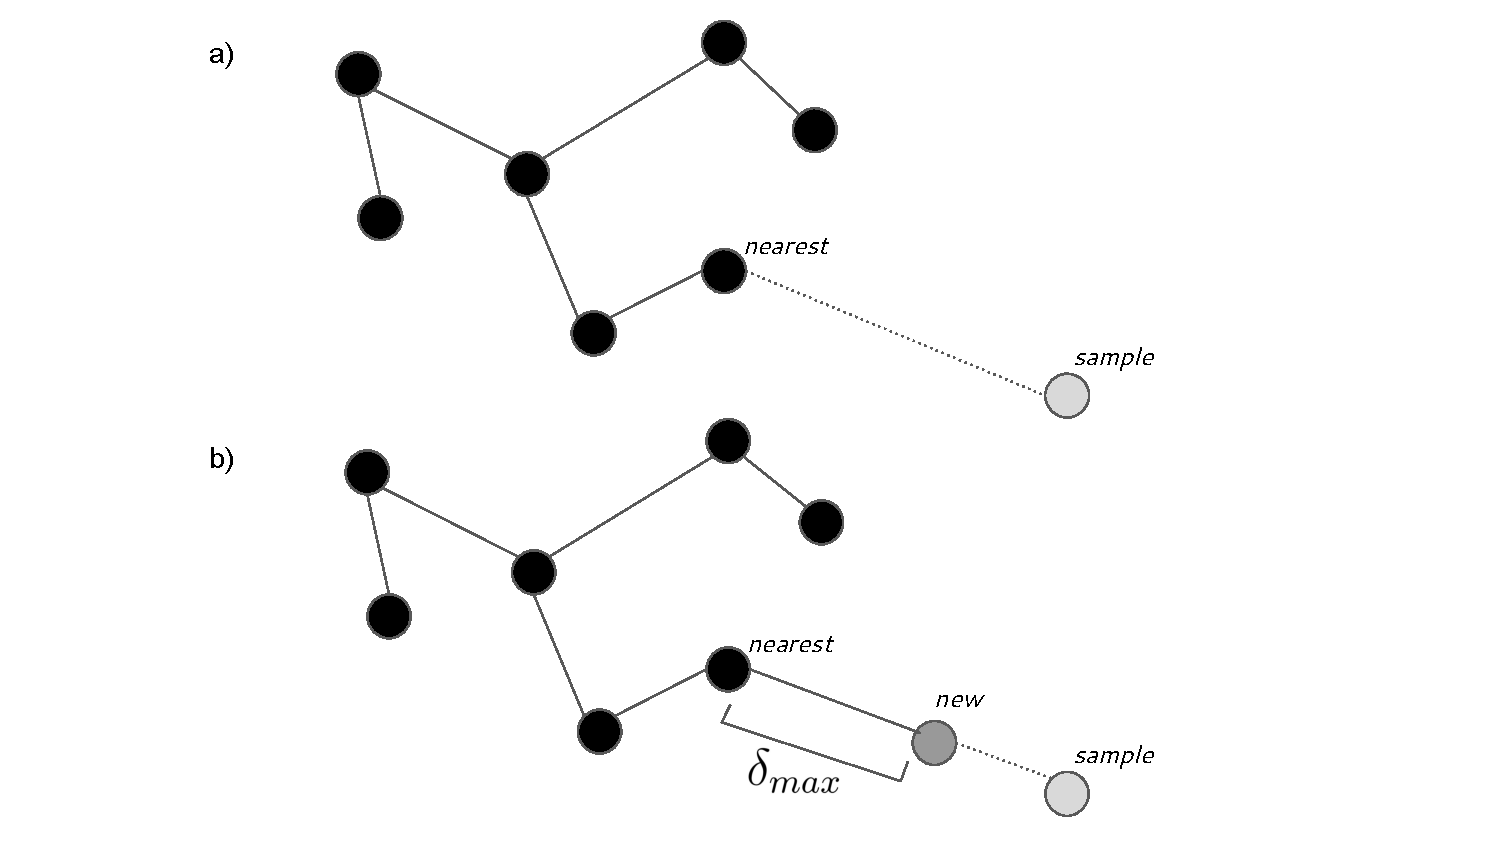
\includegraphics[width=\textwidth]{./figures/RRT_figure.pdf}
    \end{center}
    \caption[RRT sampling and connection procedure]{\gls{rrt} sampling and connection procedure. The existing tree is shown with black nodes and solid edges.\ $\text{a}\rparen$ A node is randomly sampled from the state space, and the nearest existing node is found.\ $\text{b}\rparen$ A new node and edge are added to the tree along the line connecting the nearest and sampled nodes, but at a maximum distance $\delta_{max}$ from the nearest node.}
\label{rrt}
\end{figure}

An important concept in motion planning literature is {\em completeness}, and we say that an algorithm is complete if, for any input, it correctly returns in finite time whether or not there exists a solution to the path planning problem~\cite{LaValle2006}. Clearly, due to the nature of sampling-based algorithms, completeness cannot be achieved. There are, however, weaker notions of completeness which can be useful to study. One common alternative when using a random sampling scheme is the the notion of {\em probabilistic completeness}, which means that the probability that the algorithm finds a solution (if one exists) converges to 1 as the number of samples tends to infinity. Similarly, we that a motion planning algorithm is {\em asymptotically\/optimal} if the probability of finding an optimal solution (based on a preestablished cost function) approaches $1$ as the number of samples approaches infinity~\cite{Karaman2011}.

% TODO: MORE



%%%%%%%%%%%%%%%%%%%%%%%%%%%%%%%%%%%%%%%%%%%%%%%%%%%%%%%%%%%%%%%%%%%%%%%%%%%%%%%%
%%%%%%%%%%%%%%%%%%%%%%%%%%%%%%%%%%%%%%%%%%%%%%%%%%%%%%%%%%%%%%%%%%%%%%%%%%%%%%%%
\section{Temporal Logic}
%%%%%%%%%%%%%%%%%%%%%%%%%%%%%%%%%%%%%%%%%%%%%%%%%%%%%%%%%%%%%%%%%%%%%%%%%%%%%%%%
%%%%%%%%%%%%%%%%%%%%%%%%%%%%%%%%%%%%%%%%%%%%%%%%%%%%%%%%%%%%%%%%%%%%%%%%%%%%%%%%


Motion planning occurs on various levels of abstraction. A hierarchical control structure would typically have some ``vague'', high-level description of what the robot or system is supposed to do at the top, guiding the desired behaviour. Below that there is a model, usually encompassing system dynamics, with a control architecture that prescribes how information is passed along in a series of inputs and outputs, which ultimately generates a motion plan to be followed. At the lowest levels, algorithms are used to put the motion plan in action, using a tracking controller (typically with some form of feedback to improve robustness) that determines exactly what inputs ought to be applied to maneuver along the planned path trajectory.

Temporal logics are the language used to express the high-level specifications that preside over the control hierarchy, dictating what the user desires. Most instances of motion planning seek simply to move from one location to another, without any other instructions (except to avoid obstacles). This goal is often hard-coded into the algorithms designed for solving motion planning problems. However, there exists a much broader world of possibility, and allowing users to specify exactly what is desired of a robot opens many avenues for real-world applications, not to mention the benefit of having performance guarantees from the use of formal methods~\cite{Lin2014}. We choose to work with \mucalc{} is a highly expressive temporal logic which permits more diverse and complex specifications than the most widely used temporal logics, including \gls{ltl}, \gls{ctl}, and extensions thereof~\cite{Karaman2009}, as well as for the relative ease and elegance of model checking that it permits. An in-depth background on \mucalc{} is provided \autoref{chap:prelims}.

% TODO: MORE?


%%%%%%%%%%%%%%%%%%%%%%%%%%%%%%%%%%%%%%%%%%%%%%%%%%%%%%%%%%%%%%%%%%%%%%%%%%%%%%%%
%%%%%%%%%%%%%%%%%%%%%%%%%%%%%%%%%%%%%%%%%%%%%%%%%%%%%%%%%%%%%%%%%%%%%%%%%%%%%%%%
\section{Contributions}
%%%%%%%%%%%%%%%%%%%%%%%%%%%%%%%%%%%%%%%%%%%%%%%%%%%%%%%%%%%%%%%%%%%%%%%%%%%%%%%%
%%%%%%%%%%%%%%%%%%%%%%%%%%%%%%%%%%%%%%%%%%%%%%%%%%%%%%%%%%%%%%%%%%%%%%%%%%%%%%%%

Summarizing the contributions of this thesis, we have successfully solved a kinodynamic planning problem with temporal logic specifications without the need for a solution to an \gls{obvp}, also called a steering function. While using temporal logic specifications with motion planning has been heavily researched, e.g.,~\cite{Ayala2013, Bhatia2010, Karaman2009,Lin2014, Wolff2014}, it is often difficult or impossible to find a steering function, allowing motion planning only for simple dynamical systems. Addressing this issue, we have developed a means of combining the asymptotically optimal and probabilistically complete kinodynamic planning algorithm \gls{sst}* (see \autoref{prelims:sst}) from~\cite{Li2016} with the model checking procedure from~\cite{Karaman2009} to create a motion planning algorithm with deterministic \mucalc{} specifications that does not rely on a steering function. By merging information obtained from multiple Kripke structures, we are able to create one \emph{abstracted Kripke structure} which stores the most cost-efficient paths that reach other proposition regions of the state space. To connect the trajectories found from multiple Kripke structures, an \gls{lqr} feedback control policy is used to track the candidate trajectories stored in the abstracted Kripke structure. Simulations demonstrate that it is possible to satisfy a complex liveness specification for infinitely often reaching three regions of state space using only forward propagation.

Furthermore, we use the notion of an abstracted Kripke structure to solve the planning problem with temporal logic specifications on the highly nonlinear quadrotor system. % TODO: abstract kripke + FMT

An introductory overview of \mucalc{} is conducted in \autoref{chap:prelims} which is intended to be both detailed and understandable. Many early papers on the subject are cited and amalgamated into one section to provide readers with a deep intuition on the subject of temporal logic using \mucalc{}. Deterministic \mucalc{} receives particular attention due to its impressive expressiveness coupled with its propensity for fast model checking.

We also provide many details and clarifying explanations that are missing from some of the key papers regarding quadrotor motion planning, including quadrotor dynamics~\cite{Mellinger2011}, real-time planning~\cite{Allen2016}, and geometric control methods~\cite{Lee2010}, in \autoref{chap:quad}. Much of the literature in this area focuses on the engineering aspects or provides too little (or convoluted) justification for results; in contrast, we take a deeper look at the mathematics involved in deriving many of the equations that arise in kinodynamic planning for quadrotors. Moreover, the provided level of detail should be sufficient in guiding the interested reader to implement the algorithms and frameworks discussed herein.


%%%%%%%%%%%%%%%%%%%%%%%%%%%%%%%%%%%%%%%%%%%%%%%%%%%%%%%%%%%%%%%%%%%%%%%%%%%%%%%%
%%%%%%%%%%%%%%%%%%%%%%%%%%%%%%%%%%%%%%%%%%%%%%%%%%%%%%%%%%%%%%%%%%%%%%%%%%%%%%%%
\section{Overview}
%%%%%%%%%%%%%%%%%%%%%%%%%%%%%%%%%%%%%%%%%%%%%%%%%%%%%%%%%%%%%%%%%%%%%%%%%%%%%%%%
%%%%%%%%%%%%%%%%%%%%%%%%%%%%%%%%%%%%%%%%%%%%%%%%%%%%%%%%%%%%%%%%%%%%%%%%%%%%%%%%

The rest of this thesis is structured as follows. \autoref{chap:prelims} introduces many of the important and recurring concepts discussed throughout. The syntax and semantics of \mucalc{} are provided, and a crucial theorem used in model checking is stated with proof. Then, the fragment of \mucalc{} we will use, called deterministic \mucalc{}, is defined. Lastly, many common specifications are described in detail to provide the foundations of the language of our temporal logic specifications. We then move to a description of the kinodynamic planning algorithm \gls{sst}* which we will use in \autoref{chap:sstpaper}. The final section of this chapter provides a detailed look at the \gls{fmt} algorithm, which we use for quadrotor motion planning.

The next chapter (\autoref{chap:sstpaper}) demonstrates novel research on solving kinodynamic planning problems while satisfying deterministic \mucalc{} specifications without requiring a steering function. A problem statement is provided along with a detailed description of the meta-algorithm \texttt{KinoSpecPlan} which combines using \gls{sst}* with a local deterministic model checking algorithm as well as \gls{lqr} tracking. A complex liveness specification is then shown to be satisfied in an example that uses this method.

\autoref{chap:quad} focuses on the application of kinodynamic planning to quadrotors. The dynamics of a quadrotor system are derived, and the problem of planning with deterministic \mucalc{} specifications is stated. We then outline all of the necessary components for a real-time motion planning framework and demonstrate some simulation results for the task of transiting from an initial state to a goal state. Lastly, the ideas from \autoref{chap:sstpaper} are used in the context of quadrotor planning to produce trajectories satisfying temporal logic specifications.
%TODO: has this last part changed?

Lastly, \autoref{chap:conc} offers closing remarks as well as directions for future work.

%!TEX root = uw-ethesis.tex
% chktex-file 46 (ignore warnings about $...$)
% chktex-file 24 (ignore \label warning)
\chapter{Preliminaries}\label{chap:prelims}

In this chapter, we introduce some core background concepts that arise throughout the thesis. First, we detail the notation and specify the semantics of a our choice of temporal logic, \mucalc{}, and provide the model checking tools necessary to use it. A description of the incremental kinodynamic planning algorithm \gls{sst}* follows, along with a description of the various functions used to implement the planning algorithm. This is contrasted with \gls{fmt}, which is another motion planning algorithm that is not incremental.


%%%%%%%%%%%%%%%%%%%%%%%%%%%%%%%%%%%%%%%%%%%%%%%%%%%%%%%%%%%%%%%%%%%%%%%%%%%%%%%%
%%%%%%%%%%%%%%%%%%%%%%%%%%%%%%%%%%%%%%%%%%%%%%%%%%%%%%%%%%%%%%%%%%%%%%%%%%%%%%%%
\section{\texorpdfstring{$\mu$-Calculus}{mu-Calculus}}
%%%%%%%%%%%%%%%%%%%%%%%%%%%%%%%%%%%%%%%%%%%%%%%%%%%%%%%%%%%%%%%%%%%%%%%%%%%%%%%%
%%%%%%%%%%%%%%%%%%%%%%%%%%%%%%%%%%%%%%%%%%%%%%%%%%%%%%%%%%%%%%%%%%%%%%%%%%%%%%%%

We begin by defining the syntax and semantics of the full, modal \mucalc{}. A simple example Kripke structure is provided to build some intuition surrounding the notation and meaning of some common \mucalc{} formulas. We then describe a fragment of \mucalc{} called deterministic \mucalc{}, which we will be using for the motion planning procedure in \autoref{chap:sstpaper}. Finally, we present many examples of typical deterministic \mucalc{} formulas, describing how to parse and thoroughly understand each one.



%%%%%%%%%%%%%%%%%%%%%%%%%%%%%%%%%%%%%%%%%%%%%%%%%%%%%%%%%%%%%%%%%%%%%%%%%%%%%%%%

\subsection{\texorpdfstring{Modal $\mu$-Calculus}{Modal mu-Calculus} }
First, an atomic proposition is a declarative statement that is either true or false, and which cannot be further split into smaller statements. An example of an atomic proposition might be ``in free space'', where a state satisfies the atomic proposition if and only if it lies in the defined free space for a problem. On the other hand, the statement ``in free space AND not in goal region'' is not an atomic proposition, as it can be further deconstructed into the simpler statements ``in free space'' and ``in goal region''. As this example demonstrates, more complex statements use logical connectives such as conjunction ($\land$, logical AND), disjunction ($\lor$, logical OR), and negation ($\lnot$, logical NOT). We will also be using the modal operators $\Diamond$ and $\square$, and the symbols $\mu$ and $\nu$ as least and greatest fixed point operators, respectively. Definitions for these fixed point operators will be provided.

Let $\Pi$ be the set of atomic propositions, and let $\Var$ be the set of variables. Then we define the following structure as in~\cite{Karaman2009}.
\begin{defn}\label{defn:kripke}
    A \emph{Kripke structure} $K$ over the set of atomic propositions $\Pi$ is a tuple $(S,S_0,R,\mathcal{L})$ where $S$ is a finite set of states, $S_0 \subseteq S$ is a set of initial states,  $R \subseteq S \times S$ is a binary relation which indicates a means of transiting from one state to another (usually represented as the edges in a directed graph), and $\mathcal{L}:S \to 2^\Pi$ is a labeling function, mapping each state to the subset of propositions that it satisfies.
\end{defn}

In essence, a Kripke structure is a graph with edges representing available transitions between nodes, which represent states that have been added to the graph via some sampling scheme. The distinction to be made between a Kripke structure and any other graph representation is that every node on the graph has an associated label which defines which atomic propositions that node satisfies. \autoref{fig:kripke} is an example of graph that could represent a Kripke structure.
The set of states, $S$, is represented by the nodes of the graph, the set of initial states is given by the singleton containing the bottom-left node, and the set of relations is represented by the edges. Define $\pi_f$ to be the atomic proposition ``in free space'', $\pi_g$ to mean ``in goal'', and $\pi_o$ to mean ``in obstacle''. The labeling function would then simply specify, for every node, the subset of $\Pi = \{ \pi_f, \pi_g, \pi_o \}$ that it satisfies.

\begin{figure}[!ht]
    \begin{center}
        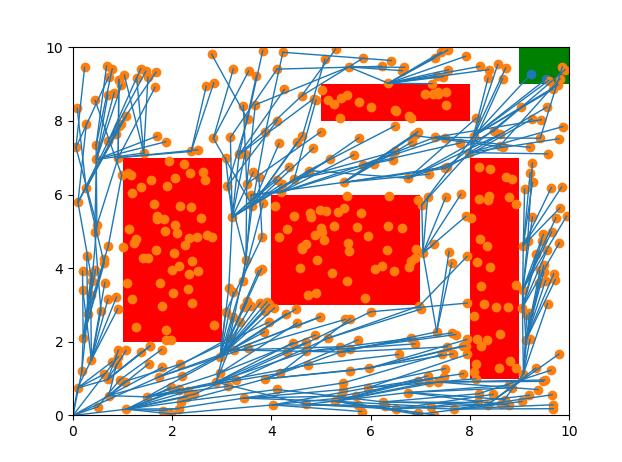
\includegraphics[width=0.85\textwidth]{./figures/kripke_example}
    \end{center}
    \caption[Example of a Kripke structure]{Example of a Kripke structure, with obstacles shown in red, free space shown in white, and the goal set shown in green.}
\label{fig:kripke}
\end{figure}


\noindent Define the set of valid \mucalc{} formulas ($L_\mu$) inductively, as follows:
\begin{itemize}
    \item the symbols \true{} and \false{} are formulas;
    \item every $p \in \Pi$ and $X \in \Var$ is a formula;
    \item if $\phi,\psi$ are formulas, then $\lnot \phi$, $\phi \land \psi$, and $\phi \lor \psi$ are also formulas;
    \item if $\phi$ is a formula then $\Diamond \phi$ and $\square \phi$ are formulas;
    \item if $\phi[X]$ is a formula where $\phi[X]$ is syntactically monotone in $X$, then $\mu X.\phi$ and $\nu X.\phi$ are formulas.
\end{itemize}
As in~\cite{Gurfinkel2004}, we write $\phi[X]$ to indicate that $\phi$ may contain an occurrence of $X$.

Next, we state definitions that will prove to be useful in the discussion of model checking for our chosen fragment of \mucalc{}, deterministic \mucalc{}, which will be seen in \autoref{prelims:deterministic_mucalc}.

\begin{defn}
    Given a \mucalc{} specification, $\phi$, we say that a variable $X$ is {\em positive\/} (respectively, {\em negative\/}) if it occurs under the scope of an even (respectively, odd) number of negations in $\phi$.
\end{defn}

\begin{defn}
    A subformula $X$ is {\em pure\/} in \mucalc{} specification $\phi$ if all of its occurrences have the same polarity (i.e., all occurrences of $X$ are positive or all occurrences of $X$ are negative).
\end{defn}

\begin{defn}
    The formula $\phi[X]$ is {\em syntactically\/monotone} in $X$ if and only if $X$ occurs with pure polarity in $\phi$.
\end{defn}


\mucalc{} formulas are interpreted with respect to a Kripke structure $K = (S,S_0,R,\mathcal{L})$ and an {\em environment\/} (also called an {\em evaluation\/}), $e: \Var \to 2^S$, which initializes (i.e., assigns a subset of $S$ to) each free variable, where a free variable is defined in the usual sense and a variable is otherwise said to be bound by a fixed point operator. For every $L_\mu$ formula $\phi$, given a Kripke structure, $K$, define $\brackets{\phi}_K^e \subseteq S$ to be the set of states of $S$ satisfying proposition $\phi$ (note that the subscript $K$ is often omitted when the Kripke structure being used is clear, and the superscript $e$ is omitted when $\phi$ contains no free variables). The semantics of the formulas is determined inductively by the following, where $p \in \Pi$, $X \in \Var$, and $\phi, \psi \in L_\mu$ are arbitrary formulas~\cite{Wilke2001}.

\begin{tabular}{l}
    $\lb \false \rb_K = \emptyset$ \\
    $\lb \true \rb_K = S$ \\
    $\brackets{p}_K = \{s \in S : p \in \mathcal{L}(s) \}$ \\    
    $\lb \lnot p \rb_K = S \setminus \lb p \rb$ \\
    $\brackets{\phi \lor \psi}_K^e = \brackets{\phi}_K^e \cup \brackets{\psi}_K^e $ \\ 
    $\brackets{\phi \land \psi}_K^e = \brackets{\phi}_K^e \cap \brackets{\psi}_K^e $ \\
    $\brackets{\Diamond \phi}_K^e = \Pree{\phi}$ \\
    $\brackets{\square \phi}_K^e = \Prea{\phi}$ \\
    $\brackets{\mu X. \phi}_K^e = \bigcap \{ A \subseteq S : \brackets{\phi}_K^{e[X \leftarrow A]} \subseteq A \}$ \\
    $\brackets{\nu X. \phi}_K^e = \bigcup \{ A \subseteq S : \brackets{\phi}_K^{e[X \leftarrow A]} \supseteq A \}$
\end{tabular}

\vspace*{2.2mm}
\noindent
The existential and universal {\em predecessor\/} functions $\text{Pre}_{K,\ \cdot}^e:L_\mu \to S$ map a \mucalc{} formula to the set of states which immediately precede (i.e., have transitions to) states satisfying said formula in the Kripke structure $K$ and under evaluation $e$:
\begin{align*}
    \Pree{\phi} &:= \{ s \in S : \exists s' \in S \ \text{s.t.} \ (s,s') \in R \land s' \in \brackets{\phi}_K^e\} \\
    \Prea{\phi} &:= \{ s \in S : \forall s' \in S, (s,s') \in R \implies s' \in \brackets{\phi}_K^e\}.
\end{align*}

In words, $\true{} = (p \lor \lnot p)$ holds for all states in $S$, and $\false{} = (p \land \lnot p)$ does not hold for any state in $S$; disjunction and conjunction of formulas is equivalent to the union and intersection of the sets which satisfy them, respectively; $\Diamond$ is the {\em existential\/successor} (or ``next'') operator, and $\square$ is the {\em universal\/successor} operator; lastly, $\mu$ and $\nu$ are the {\em least\/} and {\em greatest\/fixed-point} operators, respectively, where $e[X \leftarrow A]$ is a modified evaluation function which maps $X$ to $A$, i.e., $e[X \leftarrow A](X) = A$. To help build a more intuitive understanding of these last four semantic definitions, a simple example is provided (\autoref{mucalc_example}).

\begin{figure}[!ht]
    \centering
    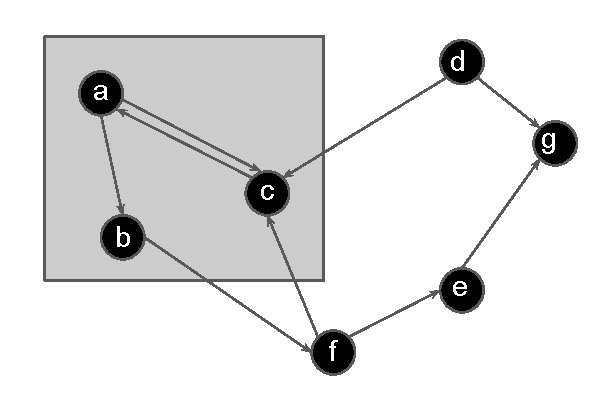
\includegraphics[width=0.6\textwidth]{./figures/mucalc_example}
    \caption[$\mu$-Calculus semantics example]{$\mu$-Calculus semantics \autoref{mucalc_example}.}
\label{fig:mucalc_example}
\end{figure}

\begin{exmp}\label{mucalc_example}
Refer to \autoref{fig:mucalc_example}.\\
Define atomic proposition $p$ to be the boolean value corresponding to ``in gray region''. Then we can specify the labeling function for each node, writing $\mathcal{L}(s_p) = \{p\}$ for nodes $s_p \in \{a, b, c\}$, and $\mathcal{L}(s) = \emptyset$ for nodes $s \in \{d, e, f, g \}$. Note that the environment superscript $e$ is omitted as we are not using any free variables.

\begin{tabular}{l}\label{table:modal_mucalc_syntax}
    $\brackets{p}_K = \{s \in S : p \in \mathcal{L}(s) \} = \{a, b, c\}$ \\    
    $\lb \lnot p \rb_K = S \setminus \lb p \rb$ = \{d, e, f, g \} \\
    $\brackets{\Diamond p}_K = \Pree{p} = \{a, c, d, f\}$ \\
    $\brackets{\square p}_K = \Prea{p}$ = \{a, c\} \\
    $\brackets{\mu X.(p \lor \Diamond X)}_K = \bigcap \{ A \subseteq S : \brackets{\phi}_K^{e[X \leftarrow A]} \subseteq A \} = \{ a,b,c,d,f \}$ \\
    $\brackets{\nu X.(p \land \Diamond X)}_K = \bigcup \{ A \subseteq S : \brackets{\phi}_K^{e[X \leftarrow A]} \supseteq A \} = \{ a, c \}$
\end{tabular}
\begin{itemize}
    \item $\brackets{p}_K$ is the set of nodes satisfying $p$ (nodes in the gray region).
    \item $\lb \lnot p \rb_K$ is the complement of $\brackets{p}_K$ in $S$ (nodes that are not in the gray region).
    \item $\brackets{\Diamond p}_K$ contains those nodes that have a transition to a node satisfying $p$.
    \item $\brackets{\square p}_K$ contains only nodes such that every transition leads to a node satisfying $p$.
    \item $\brackets{\mu X.(p \lor \Diamond X)}_K$ is the ``Reachability'' specification (see \autoref{prelims:spec_examples}). In this case, the resulting set consists of the nodes that are in the gray region \emph{or} that can take transitions to eventually reach a node in the gray region.
    \item $\brackets{\nu X.(p \land \Diamond X)}_K$ is the ``Safety'' specification (see \autoref{prelims:spec_examples}). In this case, the resulting set consists of the nodes that are in the gray region \emph{and} can always take a transition to a node that is also in the gray region. 
\end{itemize}

\end{exmp}

In order to develop a means to evaluate expressions containing fixed-point operators, we rely on the Tarski-Knaster theorem from set theory. The next section introduces some definitions before stating the required theorem.




%%%%%%%%%%%%%%%%%%%%%%%%%%%%%%%%%%%%%%%%%%%%%%%%%%%%%%%%%%%%%%%%%%%%%%%%%%%%%%%%

\subsection{Tarski-Knaster Theorem}

The Tarski-Knaster fixed-point theorem (\autoref{thm:tarski}) we introduce in this section makes an important statement about complete lattices and their fixed-points~\cite{Tarski1955}. We make use of this theorem to formulate an algorithm which computes the least or greatest fixed points for the set of states satisfying a \mucalc{} proposition containing a least or greatest fixed point operator. Note that if a proposition does not contain fixed point operators or the existential successor operator, it is easy to evaluate the set of states satisfying such a proposition. We begin by defining the necessary concepts.

\begin{defn}
    Let $(X, \leq)$ be a partially ordered set, and let $A \subseteq X$. Then $\bigvee A$ ($\bigwedge A$) denotes the least upper bound (respectively, greatest lower bound) of $A$ with respect to $\leq$, if it exists. We say that $X$ is a {\em complete\/lattice} if, for every $A \subseteq X$, then both $\bigvee A$ and $\bigwedge A$ exist in $X$.
\end{defn}

\begin{exmp}\label{ex_complat}
Consider $(\mathcal{P}(X), \subseteq)$ for any set $X$, where $\mathcal{P}(X)$ denotes the power set of $X$. Note that $\forall A \subseteq \mathcal{P}(X), \ \bigvee A = \bigcup A$, since the union of all the elements of $A$ gives the smallest set which completely contains the elements of each subset in $A$, and this union must be an element of $\mathcal{P}(X)$. Similarly, $\bigwedge A = \bigcap A \in \mathcal{P}(X)$. Thus, $(\mathcal{P}(X), \subseteq)$ is a complete lattice.
\end{exmp}

\begin{defn}
Let $(A, \leq_A)$ and $(B, \leq_B)$ be partially ordered sets. A function $f : A \to B$ is {\em monotone\/} if $a_1 \leq_A a_2 \implies f(a_1) \leq_B f(a_2)$.\\
A point $a \in A$ is a {\em fixed\/point} of a function $f: A \to B$ if $f(a) = a$, and we denote the set of all fixed points of $f$ by $\textsc{fix}(f)$.
\end{defn}

\begin{thm}\label{thm:tarski}
    \text{\normalfont(Tarski-Knaster Fixed Point Theorem)}~\\
    Let $\mathbb{L}$ be a complete lattice and let $F: \mathbb{L} \to \mathbb{L}$ be monotone. Then
    \begin{enumerate}
    \item $\bigvee \{ x \in \mathbb{L} \ \vert \ x \leq F(x) \} \in \textsc{fix}(F)$,
    \item $\bigwedge \{ x \in \mathbb{L} \ \vert \ F(x) \leq x \} \in \textsc{fix}(F)$, and
    \item $\textsc{fix}(F)$ is a complete lattice.
    \end{enumerate}
\end{thm}

\begin{proof}~\\
    Let $\mu F := \{ u \in \mathbb{L} \ \vert \ u \leq F(u) \}$, and
    let $\zeta = \bigvee \mu F$ ($\zeta$ exists since $\mu F \subseteq \mathbb{L}$, a complete lattice).
    For all $u \in \mu F$, $u \leq \zeta$, so $u \leq F(u) \leq F(\zeta)$, by monotonicity.
    Thus, $F(\zeta)$ is an upper bound for $\mu F$, and $\zeta$ is the least upper bound, so $\zeta \leq F(\zeta)$.
    By monotonicity, $F(\zeta) \leq F(F(\zeta))$, so $F(\zeta) \in \mu F$. This implies that that $F(\zeta) \leq \zeta$.
    Therefore, $\zeta = F(\zeta) \in \textsc{fix}(F)$.
    A similar argument can be made for $\bigwedge \{ u \in \mathbb{L} \ \vert \ F(u) \leq u \}$.

    Now we show that an arbitrary subset $A \subseteq \textsc{fix}(F)$ has a least upper bound and a greatest lower bound, thereby proving $\textsc{fix}(F)$ is a complete lattice.
    Define $a:=\bigvee A$, and $1_\mathbb{L} = \bigvee \mathbb{L}$.
    Consider the interval $[a,1_\mathbb{L}] := \{ x \in \mathbb{L} \ \vert \ a \leq x \leq 1_\mathbb{L} \}$, which is a complete lattice.
    Then if $A$ has a least upper bound in $\textsc{fix}(F)$, it must lie in $[a,1_\mathbb{L}]$.
    Note that it suffices to show that $F$ can be restricted to act as a monotone function
    $F:[a,1_\mathbb{L}] \to [a,1_\mathbb{L}]$, so that we may apply the first result: a monotone function on the complete lattice $[a,1_\mathbb{L}]$ has a least fixed point, and this point is therefore the least upper bound of $A \subseteq \textsc{fix}(F)$.
    Let $x \in A$. Then $x \leq a$ and $x = F(x) \leq F(a) = a$ by monotonicity, so $a \leq F(a)$.
    Letting $y \in [a,1_\mathbb{L}]$, we can see that $a \leq y$ and $a = F(a) \leq F(y) \leq 1_\mathbb{L}$ by monotonicity.
    This implies $F(y) \in [a,1_\mathbb{L}]$, so we conclude that $F([a,1_\mathbb{L}]) \subseteq [a,1_\mathbb{L}]$ which further implies that we may restrict the domain and co-domain, $F: [a,1_\mathbb{L}] \to [a,1_\mathbb{L}]$.
    We have thus shown that an arbitrary subset $A \subseteq \textsc{fix}(F)$ has a least upper bound in $\textsc{fix}(F)$. It is true for all lattices $\mathbb{L}$ that if every sublattice $S \subseteq \mathbb{L}$ has a least upper bound $\bigvee S$, then $S$ has a greatest lower bound defined by
    \[\bigwedge S = \bigvee \left( \bigcap\limits_{s \in S} \{ x \in \mathbb{L}: x \leq s \} \right).\]
    Therefore, $\textsc{fix}(F)$ is a complete lattice.
\end{proof}

We will use this theorem to perform model checking over a Kripke structure on propositions with a fixed point operator $\phi = \sigma X.\psi$, where we use $\sigma$ as a generic symbol to represent either $\mu$ or $\nu$.

\begin{cor}\label{cor:tarskialg}
    Let $K = (S,S_0,R,\mathcal{L})$ be a Kripke structure, $e: \Var \to 2^S$ be an evaluation, and $\phi \in L_1$ be a deterministic \mucalc{} formula. Define $Q_i^\mu$ and $Q_i^\nu$ recursively as follows:
    \vspace{2mm}\\
    % chktex-file 44  (disables warning for vertical line in table)
    \begin{tabular}{l | l}
        $Q_0^\mu = \emptyset$   
            & $Q_0^\nu = S$\\
        $Q_i^\mu = \brackets{\phi}_K^{e[X \leftarrow Q_{i-1}^\mu]}$ 
            & $Q_i^\nu = \brackets{\phi}_K^{e[X \leftarrow Q_{i-1}^\nu]}$
    \end{tabular}\\

    \noindent then 
    \begin{enumerate}[label = (\roman*)]   
        \item $\forall i \in \mathbb{N},\ Q_{i-1}^\mu \subseteq Q_i^\mu$ and $Q_i^\nu \subseteq Q_{i-1}^\nu$,
        \item $\exists n,m \in \mathbb{N}$ such that $Q_{n-1}^\mu = Q_n^\mu$, $Q_{m-1}^\nu = Q_m^\nu$, and
        \item $Q_n^\mu = \brackets{\mu X.\phi}_K^e$, $Q_m^\nu = \brackets{\nu X.\phi}_K^e$.
    \end{enumerate}
\end{cor}

\sref{Corollary}{cor:tarskialg} presents an intuitive algorithm for finding the least and greatest fixed points satisfying a given \mucalc{} proposition with fixed point operators. Note that the complete lattice in question is the power set of the set of states ordered by set inclusion, ${(\mathcal{P}(S), \subseteq)}$, as in \autoref{ex_complat}. The proof relies on the fact that deterministic \mucalc{} propositions are inherently {\em syntactically\/monotone} and therefore {\em monotone\/} in their variables~\cite{Gurfinkel2004}, as negation is allowed only on atomic propositions. This implies that for any formula of the form $\sigma X.\psi[X]$, $A \subseteq B$ implies $\brackets{\psi}_K^{e[X \leftarrow A]} \subseteq \brackets{\psi}_K^{e[X \leftarrow B]}$. Summarizing the algorithm, to evaluate $\brackets{\mu X.\psi}_K^e$, it suffices to set $Q_1^\mu$ to be the set of states satisfying the formula $\psi$ where $X = Q_0^\mu$ is initialized to be the empty set. We then proceed inductively, letting each subsequent $Q_i^\mu$ be the result of finding the states which satisfy $\psi$ where $X$ is replaced by $Q_{i-1}^\mu$. After a finite number $n$ of iterations (since the set of states $S$ of a Kripke structure is finite, see~\autoref{defn:kripke}), a fixed point $Q_{n-1} = Q_n = \brackets{\mu X.\psi}_K^e$ will be reached. An analogous algorithm is applied when we wish to evaluate $\brackets{\nu X.\phi}_K^e$, where $Q_0^\nu = X$ is initialized to be $S$.






%%%%%%%%%%%%%%%%%%%%%%%%%%%%%%%%%%%%%%%%%%%%%%%%%%%%%%%%%%%%%%%%%%%%%%%%%%%%%%%%

\subsection{\texorpdfstring{Deterministic $\mu$-Calculus}{Deterministic mu-Calculus}}\label{prelims:deterministic_mucalc}

We will focus our efforts on a fragment of \mucalc{} called {\em deterministic\/\mucalc{}\/} which admits efficient model-checking algorithms and is at least as expressive as the commonly used linear time temporal logics \gls{ltl} and \gls{ctl}~\cite{Karaman2009}. Deterministic \mucalc{} imposes some restrictions on syntax, notably that only atomic propositions may be negated, conjunction can only occur between a formula and an atomic proposition, and the universal successor operator $\square$ is omitted. We may write this syntax succinctly in Backus-Naur form as follows:
\[ 
\phi := p \ | \ \lnot p \ | \ X \ | \ p \land \phi \ | \ \lnot p \land \phi \ | \ \phi \lor \phi \ | \ \Diamond \phi \ | \ \mu X.\phi \ | \ \nu X. \phi
\]
where $p \in \Pi$ and $X \in \Var$. We denote the set of all deterministic $\mu$-calculus formulas by $L_1$. Note that by restricting negation to atomic propositions only, we ensure that every formula in $L_1$ is syntactically monotone in its variables.


%%%%%%%%%%%%%%%%%%%%%%%%%%%%%%%%%%%%%%%%%%%%%%%%%%%%%%%%%%%%%%%%%%%%%%%%%%%%%%%%




\subsection{Specification Examples}\label{prelims:spec_examples}

This section will introduce several examples of commonly used deterministic \mucalc{} specifications. Each example is named, described, and explained in detail to provide some intuition to the reader~\cite{Karaman2009}.

\begin{enumerate}[label = (\roman*)]
    \item \textbf{Reachability}: $\phi = \mu X.(p \lor \Diamond X)$\label{reachability_example} \\
        The reachability specification is used to ensure that the system eventually reaches a state which satisfies atomic proposition $p$. The resulting set $\brackets{\phi}_K^e$ is the {\em winning set}, that is, the set of all initial states for which the proposition $\phi$ holds. In this case, the winning set consists of states which satisfy $p$ or for which there exists a sequence of transitions in $R$ which lead to a state satisfying $p$. In the context of the Kripke structure $K = (S,S_0,R,\mathcal{L})$, we seek only to show that $S_0$ is contained in the winning set $\brackets{\phi}_K^e$.

        In this example, we look for the least fixed point because we will start with the empty set and grow through all states that satisfy $p$ or that can reach $\brackets{p}_K$ with one transition, then two transitions, and so on until the entire winning set is found. This process is guaranteed to terminate since the formula $(p \lor \Diamond X)$ is monotone ($\phi$ is a deterministic \mucalc{} formula), and since the Kripke structure contains finitely many states. Let us apply the algorithm from \sref{Corollary}{cor:tarskialg} to elucidate the procedure:
        \begin{align*}
            Q_0^\mu &= \emptyset \\
            Q_1^\mu &= \brackets{p \lor \Diamond X}_K^{e[X \leftarrow Q_0^\mu]} \\
                    &= \brackets{p}_K \cup \brackets{\Diamond X}_K^{e[X \leftarrow \emptyset]}\\
                    &= \brackets{p}_K \cup \Pree[{e[X \leftarrow \emptyset]}]{X} \\
                    &= \brackets{p}_K \cup \{ s \in S : \exists s' \in S \ \text{s.t.} \ (s,s') \in R   \land s' \in \emptyset \} \\
                    &= \brackets{p}_K\\
            Q_2^\mu &= \brackets{p \lor \Diamond X}_K^{e[X \leftarrow Q_1^\mu]} \\
                    &= \brackets{p}_K \cup \{ s \in S : \exists s' \in S \ \text{s.t.} \ (s,s') \in R \land s' \in \brackets{p}_K \}.
        \end{align*}
        This process continues until the least fixed point is reached. See \autoref{mucalc_example} for a concrete illustration of the reachability specification.

    \item \textbf{Safety}: $\phi = \nu X.(p \land \Diamond X)$\label{safety_example} \\
        We use the the term ``safety'' as this specification guarantees that a given atomic proposition will hold on some state trajectory; the atomic proposition may be concerned with being in an obstacle-free space, or it may ensure that constraints on speed or acceleration are observed, for instance. The formula $\phi$ will hold for all states which satisfy $p$ and which have transitions to states which will themselves satisfy $p$ and in turn have transitions to other states that will satisfy this same condition. For this reason, we start with the entire set of states, $S$, and repeatedly find intersections to narrow down the states until the greatest fixed point is reached.
        \begin{align*}
            Q_0^\nu &= S\\
            Q_1^\nu &= \brackets{p \land \Diamond X}_K^{e[X \leftarrow Q_0^\nu]} \\
                    &= \brackets{p}_K \cap \brackets{\Diamond X}_K^{e[X \leftarrow S]}\\
                    &= \brackets{p}_K \cap \{ s \in S : \exists s' \in S \ \text{s.t.} \ (s,s') \in R \land s' \in S\} \\
                    &= \brackets{p}_K\\
            Q_2^\nu &= \brackets{p \land \Diamond X}_K^{e[X \leftarrow Q_1^\nu]} \\
                    &= \brackets{p}_K \cap \{ s \in S : \exists s' \in S \ \text{s.t.} \ (s,s') \in R   \land s' \in \brackets{p}_K\} \\
            \vdots
        \end{align*}
        See \autoref{mucalc_example} for a concrete illustration of the safety specification.


    \item \textbf{Reaching a Region Safely}: $\phi = \mu X.(\lnot q \land (p \lor \Diamond X))$\\
        One way of combining the above two specifications is to ensure that a safety condition is met while trying to reach an objective. This specification is commonly used for motion planning problems, wherein a planner searches for a trajectory which avoids obstacles (represented by states satisfying $q$), and reaches a given goal (represented by states satisfying $p$). Obstacle avoidance is guaranteed by the conjunction of the usual reachability subformula with ${\lnot q}$ so that at each iteration, we keep only those states which satisfy the reachability criterion and are not obstacles.

    \item \textbf{Reaching a Safe Region}: $\phi = \mu X.((\nu Y.(p \land \Diamond Y)) \lor \Diamond X)$\\
    Another way to combine safety and reachability is the specification to reach a region whose states always satisfy a property $p$. The subformula ${\psi = \nu Y.(p \land \Diamond Y)}$ is identical to the safety specification listed above; $\psi$ is satisfied by all initial states which give rise to trajectories that always satisfy $p$. This safety specification is wrapped in the reachability specification ${\mu X.(\psi \lor \Diamond X)}$, meaning states which satisfy $\phi$ are either in the safe region already, or can reach the safe region using a finite number of transitions.

    \item \textbf{Ordering}: $\phi = \mu X.(q \lor (p \land \Diamond X))$\\
    In both \gls{ltl} and \gls{ctl}, there is a temporal operator \textsc{U} denoting ``until'', so that $p \textsc{U} q$ is satisfied provided $p$ holds at least until $q$ holds; that is, after a finite number of transitions, $q$ must hold, and $p$ may or may not continue to hold. In \mucalc{}, we can formulate this specification by building up a set of states where either $q$ is already satisfied, or $p$ is satisfied and there exists a transition to a state satisfying ${q \lor (p \land \Diamond X)}$. Another way to interpret the formula is to distribute the disjunction to obtain ${\mu X.((q \lor p) \land (q \lor \Diamond X))}$. In this form, we observe the reachability subformula ${q \lor \Diamond X}$ (in the scope of a least fixed point operator, as usual), so we may conclude that the winning set contains states which eventually satisfy $q$, and along the way must satisfy $p$ (otherwise $q$ is already satisfied, so $p$ may or may not be satisfied).

    \item \textbf{Liveness}: $\phi = \nu Y. \mu X.((p \land \Diamond Y) \lor \Diamond X)$

    Liveness, is a specification which guarantees that atomic proposition $p$ is satisfied infinitely often. This example is the first with an alternation depth greater than one, where alternation depth refers to the level of mutually recursive least and greatest fixed point operators~\cite{Wilke2001}.
    Consider the largest proper subformula of $\phi$, $\psi = {\mu X.((p \land \Diamond Y) \lor \Diamond X)}$. This can be seen as a reachability specification where the goal is to eventually reach states satisfying $\eta = p \land \Diamond Y$, which itself looks like a safety specification, remarking that $\eta$ is in the scope of a greatest fixed point operator. We may parse the liveness specification $\phi = {\nu Y.\psi} = {\nu Y.\mu X.(\eta \lor \Diamond X)}$ as follows: $\psi$ ensures that a region satisfying ${\eta = p \land \Diamond Y}$ is reached, and $\eta$ ensures that $p$ is satisfied and that there is a transition to a state satisfying $\psi$. Having mutually recursive greatest and least fixed point operators in this way allows for this more complex combination of reachability and safety, where $\phi$ is satisfied by all states which have paths that {\it always\/eventually} reach $\brackets{p}_K$. Note that liveness is also sometimes called the {\it B\"uchi\/objective} in the context of infinite parity games, a topic closely related to \mucalc{}~\cite{Emerson1991,Karaman2012,Wilke2001}.
\end{enumerate}

%%%%%%%%%%%%%%%%%%%%%%%%%%%%%%%%%%%%%%%%%%%%%%%%%%%%%%%%%%%%%%%%%%%%%%%%%%%%%%%%
%%%%%%%%%%%%%%%%%%%%%%%%%%%%%%%%%%%%%%%%%%%%%%%%%%%%%%%%%%%%%%%%%%%%%%%%%%%%%%%%
\section{SST*}\label{prelims:sst}
%%%%%%%%%%%%%%%%%%%%%%%%%%%%%%%%%%%%%%%%%%%%%%%%%%%%%%%%%%%%%%%%%%%%%%%%%%%%%%%%
%%%%%%%%%%%%%%%%%%%%%%%%%%%%%%%%%%%%%%%%%%%%%%%%%%%%%%%%%%%%%%%%%%%%%%%%%%%%%%%%

In this section, we discuss a probabilistically complete sampling-based kinodynamic motion planning algorithm called \gls{sst} along with its asymptotically optimal variant, \gls{sst}*\footnote{Note that motion planning algorithms whose acronyms end with an asterisk (*) are usually asymptotically optimal variants of their associated algorithm.}. For completeness, the planner is summarized in this section, although further details and proofs can be found in~\cite{Li2016}.

One very useful property of \gls{sst} is that it does not rely on having the solution to an \gls{obvp} for the relevant system. Such a solution is called a steering function\footnote{Some authors use different terminology for the steering/OBVP problem. For instance, in their paper on \gls{prm}, Kavraki et al.\ refer to a ``local planner'' which is used to connect neighbouring nodes in the case of \emph{holonomic} robots.} in the literature, and many motion planning algorithms are contingent upon its availability. For example, some planning algorithms that necessitate using a steering function include \gls{rrt}*~\cite{Karaman2011} and \gls{prm}~\cite{Kavraki1996}. The steering function provides, as the name suggests, optimal inputs to control or \emph{steer} the system from one given state to another; for many planners, the necessity of such a function arises when sampled states (nodes) must be connected together with directed edges, representing that there is a known set of inputs to control the system between such states. The problem is, just as finding analytic solutions to nonlinear differential equations is very difficult or impossible, so too is finding the related solution to an associated \gls{obvp}\@.

Although scarce, there are a small number of sampling-based planning algorithms that do not require a steering function, most notably RRT-Extend~\cite{LaValle2001} and \gls{est}. While \gls{est} has been shown to be asymptotically optimal (RRT-Extend is not), the rate of convergence to the (near-) optimal solution is logarithmic, making it impractical at reliably finding high-quality paths. On the other hand, the advantages offered by \gls{sst}* include being provably asymptotically optimal as well as having good (linear) convergence to high-quality solutions. \gls{sst}* is further improved by its use of a sparse data structure, where a pruning operation is used to accelerate nearest neighbours searches, thereby ameliorating computational efficiency.


We will now describe the implementation details of the \gls{sst}* sampling-based planning algorithm. \gls{sst}* employs \texttt{MonteCarlo\_Prop} which forward propagates a selected node, $x_{selected}$; that is, a random control vector is sampled from the allowed control-space, $\mathbb{U}$, and supplied as input to the system dynamics for a random duration, up to some specified maximum time, $T_{prop}$, resulting in trajectories with piecewise constant control inputs (see \autoref{alg:montecarlo}).

\begin{algorithm}
\caption{\texttt{MonteCarlo\_Prop}$(x_{selected}, \mathbb{U}, T_{prop})$}
\label{alg:montecarlo}
\begin{algorithmic}[1]
    \State{$t \gets \texttt{Sample}([0, T_{prop}])$}
    \State{$\Upsilon \gets \texttt{Sample}(\mathbb{U})$}
    \Return{$x_{new} \gets x_{selected} + \int_0^t f(x(\tau), \Upsilon) d\tau $}
\end{algorithmic}{}
\end{algorithm}


\gls{sst}* also uses a best-first selection strategy to forward integrate from the least-cost node found within a specified radius of the sampled state, thereby improving convergence to high-quality solutions. To elaborate, we use \autoref{alg:bestfirst} called \texttt{Best\_First\_Selection} to sample a random state, $x_{rand}$, from the state space, $\mathbb{X}$, then it stores in $X_{near}$ the set of all existing states in the tree within a $\delta_{BN}$ radius of $x_{rand}$. If $X_{near}$ is empty, we simply return the nearest node to $x_{rand}$ in the set of all nodes, $\mathbb{V}$. Otherwise, the state in $X_{near}$ with the least cost is selected. In either case, the selected state, $x_{selected}$, is the state from which we propagate and grow the tree using \texttt{MonteCarlo\_Prop}.
% Note that, upon collision with an obstacle during propagation, no new nodes are added to the tree and we simply proceed to the next iteration.

\begin{algorithm}
\caption{\texttt{Best\_First\_Selection}$(\mathbb{X}, \mathbb{V}, \delta_{BN})$}
\label{alg:bestfirst}
\begin{algorithmic}[1]
    \State{$x_{rand} \gets \texttt{Sample-State}(\mathbb{X})$}
    \State{$X_{near} \gets \texttt{Near}(\mathbb{V}, x_{rand}, \delta_{BN})$}
    \If{$X_{near} == \emptyset$}
        \Return{$\texttt{Nearest}(\mathbb{V}, x_{rand})$}
    \Else{}
        \Return{$\argmin_{x \in X_{near}} \texttt{Cost}(x)$}
    \EndIf{}
\end{algorithmic}{}
\end{algorithm}



\begin{figure}[!ht]
    \centering
    \includegraphics[scale=0.28]{./figures/trueflappy_1}
    \caption[SST Flappy Bird Example]{An example of a tree produced by \gls{sst} for the flappy bird problem. The initial state is in the top-left, the point travels at a constant horizontal velocity, and the control-space is a set containing only two options: ``do nothing'', or ``accelerate up'', each for a random duration. The least-cost solution for this execution is highlighted in pink.}
\label{fig:flappy}
\end{figure}

Furthermore, \gls{sst}* applies a pruning operation to maintain a sparse data structure. Pruning removes high-cost nodes to improve run-time by accelerating nearest neighbour searches. With this in mind, a graph of witness nodes is maintained, where each witness keeps track of an optimal-cost representative node within a $\delta_s$-radius of the witness. Correspondingly, we must determine whether a new node is the ``best'' in its neighbourhood in order to decide whether or not to keep it. For this purpose, we use \texttt{Is\_Locally\_Best} presented in \autoref{alg:locallybest}. The algorithm finds the nearest witness state, $s_{new}$, to the newly propagated state $x_{new}$. If $s_{new}$ is not within distance $\delta_s$ of $x_{new}$, $x_{new}$ is deemed locally best by default and becomes a new witness node. In this way, $x_{new}$ is added to the set of witness nodes, $S$. If $x_{new}$ does have a neighbour within a $\delta_s$ radius, the chosen cost function, \texttt{Cost}, is used to check whether the new state is better than the locally best representative of the witness node.

\begin{algorithm}
\caption{\texttt{Is\_Locally\_Best}$(x_{new}, S, \delta_s)$}
\label{alg:locallybest}
\begin{algorithmic}[1]
    \State{$s_{new} \gets \texttt{Nearest}(S, x_{new})$}
    \If{$\texttt{dist}(x_{new}, s_{new}) > \delta_s$}
        \State{$S \gets S \cup \{ x_{new} \}$}
        \State{$s_{new} \gets x_{new}$}
        \State{$s_{new}.rep \gets \texttt{NULL}$}
    \EndIf{}
    \State{$x_{peer} \gets s_{new}.rep $}
    \If{$x_{peer} == \texttt{NULL} \hspace{2mm} \text{or} \hspace{2mm}
        \texttt{Cost}(x_{new}) < \texttt{Cost}(x_{peer})$}
        \Return{$\texttt{True}$}
    \EndIf{}
    \Return{\texttt{False}}
\end{algorithmic}{}
\end{algorithm}

Now that there is a means of determining whether a state is locally best, we are ready to define the algorithm which enforces sparsity, \texttt{Prune} (\autoref{alg:prune}). First, the nearest witness state, $s_{new}$, to the newly propagated state, $x_{new}$, is found. We want to set $x_{new}$ to be the representative of $s_{new}$ since it has been deemed locally best if the \gls{sst}* algorithm has reached this point (see \autoref{alg:sst}), but first we must check whether or not $s_{new}$ already has a representative. Since \texttt{Prune} is only executed if \texttt{Is\_Locally\_Best} returns \texttt{True}, then if $s_{new}$ has a representative, it must have higher cost than $x_{new}$, and it must now be moved from $\mathbb{V}_{active}$ to $\mathbb{V}_{inactive}$. The next step is to remove inactive leaf nodes recursively, so that if the previous representative of $s_{new}$ is an inactive leaf node, it is removed entirely from the set of all nodes, $\mathbb{V}$, and the check is preformed again with the parent of the removed leaf node.


\begin{algorithm}
\caption{\texttt{Prune}$(x_{new}, \mathbb{V}_{active}, \mathbb{V}_{inactive}, \mathbb{E})$}
\label{alg:prune}
\begin{algorithmic}[1]
    \State{$s_{new} \gets \texttt{Nearest}(S, x_{new})$}
    \State{$x_{peer} \gets s_{new}.rep$}
    \If{$x_{peer} \neq \texttt{NULL} $}
        \State{$\mathbb{V}_{active} \gets \mathbb{V}_{active} \setminus \{ x_{peer} \}$}
        \State{$\mathbb{V}_{inactive} \gets \mathbb{V}_{inactive} \cup \{ x_{peer} \}$}
    \EndIf{}
    \State{$s_{new}.rep \gets x_{new}$}
    \While{$\texttt{IsLeaf}(x_{peer}) \hspace{2mm} \text{and} \hspace{2mm}
            x_{peer} \in \mathbb{V}_{inactive} $}
        \State{$x_{parent} \gets x_{peer}.parent $}
        \State{$\mathbb{E} \gets \mathbb{E} \setminus \{ \overline{x_{parent} \to x_{peer}} \} $}
    \EndWhile{}
    \State{$\mathbb{V}_{inactive} \gets \mathbb{V}_{inactive} \setminus \{ x_{peer} \}$}
    \State{$x_{peer} \gets x_{parent}$}
\end{algorithmic}{}
\end{algorithm}


\begin{algorithm}
\caption{\texttt{SST*}$(\mathbb{X}, \mathbb{U}, x_0, T_{prop}, N, \delta_{BN}, \delta_s, \xi)$}
\label{alg:sst}
\begin{algorithmic}[1]
    \State{$\mathbb{V}_{active} \gets \{x_0\}; \hspace{2mm} \mathbb{V}_{inactive} \gets \emptyset$}
    \State{$\mathbb{E} \gets \emptyset $}
    \State{$s_0 \gets x_0; \hspace{2mm} s_0\text.rep = x_0; \hspace{2mm} S \gets \{ s_0 \} $}
    \State{$j \gets 0$}
    \While{\texttt{True}}
        \For{$\text{N iterations}$}
            \State{$x_{selected} \gets \texttt{Best\_First\_Selection}(\mathbb{X}, \mathbb{V}_{active}, \delta_{BN})$}
            \State{$x_{new} \gets \texttt{MonteCarlo\_Prop}(x_{selected}, \mathbb{U}, T_{prop})$}
            \If{$\texttt{CollisionFree} (\overline{x_{selected} \to x_{new}})$}
                \If{$\texttt{Is\_Locally\_Best}(x_{new}, S, \delta_{s})$}
                    \State{$\mathbb{V}_{active} \gets \mathbb{V}_{active} \cup \{ x_{new} \}$}
                    \State{$\mathbb{E} \gets \mathbb{E} \cup \{\overline{x_{selected} \to x_{new}}\}$}
                    \State{$\texttt{Prune}(x_{new}, \mathbb{V}_{active}, \mathbb{V}_{inactive}, \mathbb{E})$}
                \EndIf{}
            \EndIf{}
        \EndFor{}
        \State{$\delta_s \gets \xi \cdot \delta_s ; \hspace{2mm}
                \delta_{BN} \gets \xi \cdot \delta_{BN}$}
        \State{$j \gets j + 1$}
        \State{$N \gets N (1 + \log(j)) \xi^{-j(d+l+1)}$}
    \EndWhile{}
    \State{$\mathbb{V} \gets \mathbb{V}_{active} \cup \mathbb{V}_{inactive} $}
    \Return{$(\mathbb{V}, \mathbb{E})$}
\end{algorithmic}{}
\end{algorithm}

With the necessary helper functions defined, the pseudocode for \gls{sst}* is outlined in \autoref{alg:sst}. Note that the nested for-loop constitutes the core of \gls{sst}, and the addition of the update step for $\delta_s$ and $delta_{BN}$ is all that is necessary to make the algorithm asymptotically optimal instead of being merely asymptotically near-optimal. This is because, if these two parameters do not tend to zero as the number of iterations goes to infinity, then there will always be some degree of sparsity, which means that not every possible solution is explored. In terms of notation, the overline indicates an edge (trajectory from one state to another), and $d, l$ denote the number of dimensions of the state space and the control space, respectively.


It is important to note that proper tuning of the parameters used in \gls{sst}* is crucial for effective path planning. The most significant parameters are $\delta_{BN}$ and $\delta_s$, which are the radii for selecting low-cost nearby nodes and for pruning in the vicinity of witness nodes, respectively. Choosing a large value of $\delta_s$ can decrease the time it takes to find an initial solution at the cost of solution quality, while choosing a large value of $\delta_{BN}$ can improve initial solution quality while increasing the time it takes to find an initial solution. Moreover, the \gls{sst}* algorithm is \emph{incremental}, meaning states are not sampled all at once, rather during each iteration a new state is sampled to incrementally grow a tree. A consequence of the incremental nature of \gls{sst}* is that there is no clear way to precompute solution trajectories for online use unless (necessarily static) obstacles and the initial state are specified exactly. In simulations, we have found that feasible trajectories can often be computed in under 10 seconds for simple linear systems with state space dimension three or lower; however, it can take several hundred seconds to compute solutions for higher-dimensional nonlinear systems.




%%%%%%%%%%%%%%%%%%%%%%%%%%%%%%%%%%%%%%%%%%%%%%%%%%%%%%%%%%%%%%%%%%%%%%%%%%%%%%%%
%%%%%%%%%%%%%%%%%%%%%%%%%%%%%%%%%%%%%%%%%%%%%%%%%%%%%%%%%%%%%%%%%%%%%%%%%%%%%%%%
\section{FMT*}
%%%%%%%%%%%%%%%%%%%%%%%%%%%%%%%%%%%%%%%%%%%%%%%%%%%%%%%%%%%%%%%%%%%%%%%%%%%%%%%%
%%%%%%%%%%%%%%%%%%%%%%%%%%%%%%%%%%%%%%%%%%%%%%%%%%%%%%%%%%%%%%%%%%%%%%%%%%%%%%%%

\gls{fmt} is an asymptotically optimal sampling-based motion planning algorithm that was specifically developed for use in high-dimensional systems~\cite{Janson2015}. In simulations, Janson et al.\ consistently found that \gls{fmt} converges to high-quality solutions faster than \gls{prm}* and \gls{rrt}* for systems with dimension from 2D to 7D. The improvements were more noticeable in higher dimensions, making \gls{fmt} a very promising algorithm for complex motion planning problems such as for those involving quadrotors, which operate in a 12D state space.

Unlike \gls{sst}*, \gls{fmt} is not an incremental algorithm. An important distinction results from this difference in algorithm design, namely that the definition of asymptotic optimality must be altered to accommodate the fact that \gls{fmt} uses a predetermined number of sampled states. As mentioned in~\ref{intro:sbmp}, the definition of asymptotic optimality essentially involves finding an optimal solution as the number of samples tends to infinity. In such case, each iteration builds upon an existing graph, refining the structure and covering more of the state space. For non-incremental algorithms, the definition of asymptotic optimality can be summarized as follows: the cost of the solution returned by an algorithm must converge in probability to the optimal cost.

For this work, we consider the kinodynamic variant of \gls{fmt} by Ross Allen and Marco Pavone called \texttt{kinoFMT}. The primary distinction lies in the fact that, due to considerations of differential constraints, there is a fundamental difference between searching for nearest backward-reachable and forward-reachable states. In the case of backward reachability, $\texttt{Near\_Backward}(x,V,J_{th})$ finds states in $V$ that can reach state $x$ without exceeding a threshold cost, $J_{th}$. In contrast, $\texttt{Near\_Forward}(x,V,J_{th})$ finds states in $V$ that can be reached by $x$ itself without exceeding $J_{th}$. See \autoref{quad:reachable_set} for further details. In fact, using a cost threshold is another deviation from the standard \gls{fmt} algorithm, which uses a distance threshold. Since kinodynamic planning is concerned with feasibility under kinematic and dynamic constraints, a simple distance metric is insufficient for determining which states are easily reachable from another state. \autoref{alg:fmt} presents the pseudocode of \texttt{kinoFMT} which is similar to the algorithm shown in~\cite{Allen2016} except for some slight changes for clarity and implementational simplicity.

% chktex-file 35  (disables warning for {max/min})
\begin{algorithm}
\caption{$\texttt{kinoFMT}(x_{init}, X_{goal}, \mathbb{X}, n, J_{th})$}
\label{alg:fmt}
\begin{algorithmic}[1]
    \State{$\V \gets \{ x_{init} \} \cup \texttt{Sample}(n, \mathbb{X})$}\label{fmt:V}
    \State{$\E \gets \emptyset $}
    \State{$W \gets \V \setminus \{ x_{init} \}; H \gets \{ x_{init} \} $}\label{fmt:WH}
    \State{$z \gets x_{init} $}
    \While{$z \notin X_{goal}$}\label{fmt:loopz1}
        \State{$N_z^{out} \gets \texttt{Near\_Forward}(z, V \setminus \{z\}, J_{th}) $}\label{fmt:z1}
        \State{$X_{near} = N_z^{out} \cap W $}\label{fmt:loopz2}
        \For{$x \in X_{near} $}\label{fmt:loopx1}        
            \State{$N_x^{in} \gets \texttt{Near\_Backward}(x, V \setminus \{x\}, J_{th}) $}
            \State{$Y_{near} \gets N_x^{in} \cap H $}\label{fmt:loopx2}
            \State{$y_{min} \gets \argmin_{y \in Y_{near}} \{ y.cost + \texttt{Cost}(\overline{y \to x}) \} $}\label{fmt:dynprogram}
            \If{$\texttt{CollisionFree} (\overline{y_{min} \to x})$}\label{fmt:col}
                \State{$\E \gets \E \cup \{ \overline{y_{min} \to x} \} $}\label{fmt:col1}
                \State{$x.cost \gets y_{min}.cost + \texttt{Cost}(\overline{y_{min} \to x}) $}
                \State{$H \gets H \cup \{x\} $}
                \State{$W \gets W \setminus \{x\} $}\label{fmt:col2}
            \EndIf{}
        \EndFor{}
        \State{$H \gets H \setminus \{z\} $}
        \If{$H == \emptyset $}\label{fmt:empty1}
            \Return{$\text{Failure} $}\label{fmt:empty2}
        \EndIf{}
        \State{$z \gets \argmin_{y \in H} \{ y.cost \} $}\label{fmt:z2}
    \EndWhile{}
    \Return{$\texttt{Path}(z, \V, \E) $}
\end{algorithmic}{}
\end{algorithm}

The main idea behind \gls{fmt} and \texttt{kinoFMT} is to use forward dynamic programming on a predetermined number of sampled states. The algorithms perform graph construction and graph search simultaneously, thus the final least-cost node lying in the goal region is already known when the algorithm terminates. In other words, by the nature of the expansion of the tree structure, the least-cost nodes on the frontier of expansion are always tracked, so that when the goal is reached, it is not necessary to search the entire tree for the optimal terminal node. Moreover, since tree structures contain no cycles, there exists a unique path from the starting node to the terminal node. \autoref{fig:fmt_example} demonstrates an example of a solution path found via \gls{fmt}.

\begin{figure}[!ht]
    \centering
    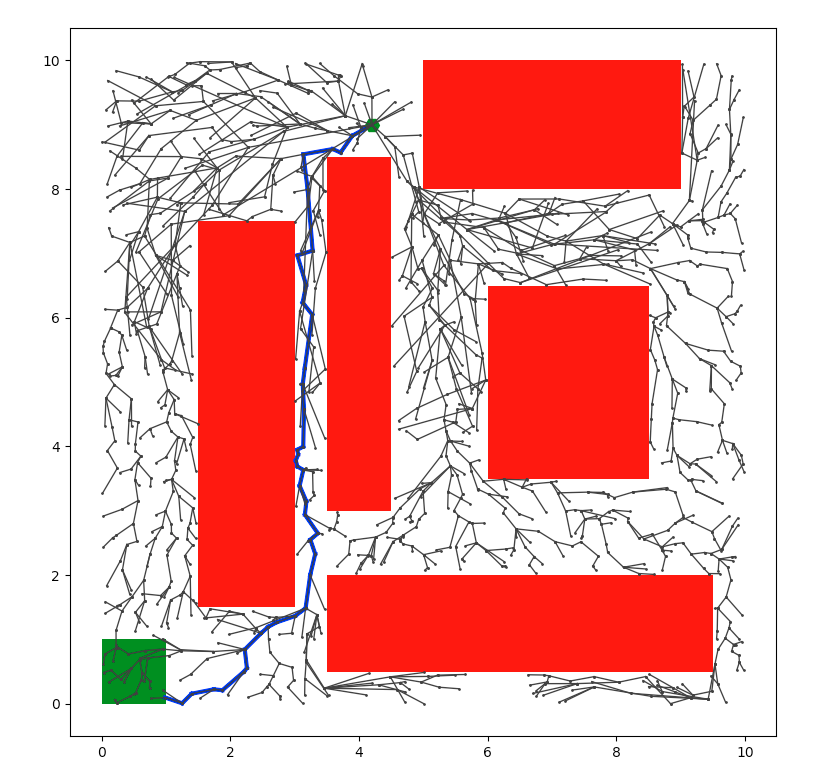
\includegraphics[scale=0.5]{./figures/fmt-2000-nodes}
    \caption[FMT* Example]{Example of a tree generated by \gls{fmt} using 2000 nodes. The initial state is shown at the top center as a green hexagon, the goal region lies in the bottom left and is shown in green, and obstacles are represented by red rectangles. The optimal path is highlighted in blue. This example does not use any dynamic model, so the cost function is simply the Euclidean distance.}
\label{fig:fmt_example}
\end{figure}

In more detail, \texttt{kinoFMT} takes as input an initial state, $x_{init}$, and goal region, $X_{goal}$, the state space, $\mathbb{X}$, the number of nodes to sample, and a cost threshold, $Jth$. The \texttt{Sample} function uniformly samples the entire state space\footnote{The \gls{fmt} algorithm specifies that samples are taken only from the free space (i.e., not including obstacles,) however, sampling from the entire state space allows for a much more general motion planning framework, as discussed in \autoref{chap:quad:rtmp}.} (usually with some samples selected directly from the goal region) and stores these sampled states in $\V$ along with $x_{init}$ (line~\ref{fmt:V}). 
The set $W$ contains unexplored nodes, and the set $H$ contains the nodes forming the frontier of expansion of the tree, which initially includes only $x_{init}$ (line~\ref{fmt:WH}). 
Every iteration, the least-cost node $z \in H$ becomes the pivot about which expansion occurs ({lines~\ref{fmt:z1},~\ref{fmt:z2}}). 
With the pivot known, we define $X_{near}$ to be the set of unexplored nearest nodes in the forward-reachable set of $z$ ({lines~\ref{fmt:loopz1}--\ref{fmt:loopz2}}). 
Then, for each element $x \in X_{near}$, define $Y_{near}$ to be the set of nodes in the frontier that are also in the backward-reachable set of $x$ ({lines~\ref{fmt:loopx1}--\ref{fmt:loopx2}}). 
The least-cost state $y_{min}$ is then found from the set of all $y \in Y_{near}$, where the cost is determined to be the sum of the cost of reaching $y$ (along its unique path from $x_{init}$) and the cost to travel from $y$ to $x$, recalling that $y$ is in the backward-reachable set of $x$ (line~\ref{fmt:dynprogram}). This is the dynamic programming step, where we try to minimize the cost-to-come and the cost-to-go. 
Once the cost minimizer is found, a collision check is performed (line~\ref{fmt:col}), and if a collision is detected along the transition from $y_{min}$ to $x$, then the algorithm simply discards this iteration and proceeds to the next. Otherwise, the edge (transition) is added to the tree, the newly connected node's cost is updated and the node is added to the frontier set, $H$, and it is simultaneously removed from the set of unexplored nodes, $W$ ({lines~\ref{fmt:col1}--\ref{fmt:col2}}). 
Once the for-loop has iterated through the entire set of forward-reachable nodes, $X_{near}$, the pivot, $z$, is removed from the frontier and the procedure repeats until either the frontier is empty, at which point ``Failure'' is returned ({lines~\ref{fmt:empty1}--\ref{fmt:empty2}}), or until $z$ lies within the goal region, at which point the algorithm terminates. 
The \texttt{Path} function simply returns the optimal path, that is, the unique path from $x_{init}$ to the final least-cost goal state, $z$.

A diagram illustrating the addition of a single transition using \gls{fmt} is provided in \autoref{fig:fmt_diagram}. In part $\text{a)}$ of the diagram, of the two nodes in the frontier, $H$, the one with least cost is selected as $z$. For this simple example, distance is used as the cost with a search radius of $J_{th}$, and three unvisited nodes are found to lie within this distance from $z$. These are the nodes belonging to $X_{near}$. The algorithm will iterate through all three nodes in $X_{near}$, but we focus on one for this example. In $\text{b)}$, we add all nodes whose search radius includes node $x$ to $N_x^{in}$. This set is not necessarily equivalent to the set of all nodes within the search radius of $x$; for non-symmetric cost functions, this distinction could have a significant impact (e.g., the \texttt{kinoFMT} algorithm). In $\text{c)}$, of the nodes in $N_x^{in}$, only those that are also in $H$ are included in the set $Y_{near}$. For each node $y \in Y_{near}$, the cost of each, $y.cost + \texttt{Cost}(\overline{y \to x})$, is computed and the least-cost node, $y_{min}$, is determined. Provided there is no collision when connecting $y_{min}$ to $x$, the edge is added to the tree and $x$ is added to the set $H$. Once this entire process is repeated for every $x \in X_{near}$, the next iteration begins with a new least-cost frontier node $z$, or returns ``Failure'' if $H$ is empty.

\begin{figure}[!ht]
    \vspace*{4mm}
    \hspace*{8mm}
    \centering
    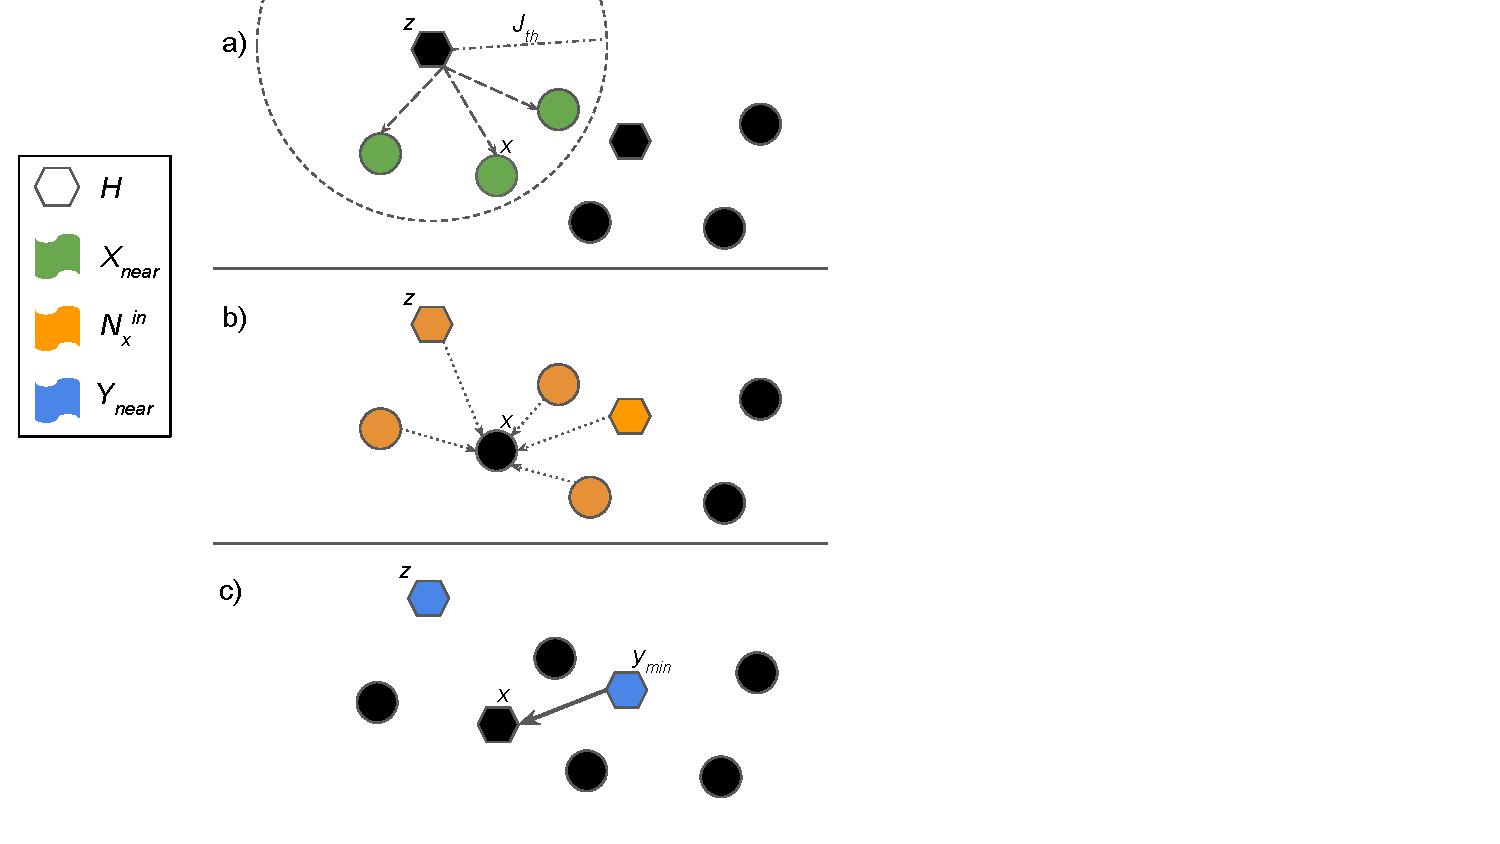
\includegraphics[scale=0.89]{./figures/fmt_diagram}
    \caption[FMT* Diagram]{
        Illustration of the \gls{fmt} algorithm.
    }
\label{fig:fmt_diagram}
\end{figure}

%!TEX root = uw-ethesis.tex
% chktex-file 46 (ignore warnings about $...$)
% chktex-file 24 (ignore \label warning)

\chapter{\texorpdfstring{Sampling-Based Motion Planning with $\mu$-Calculus Specifications without Steering}{Sampling-Based Motion Planning with mu-Calculus Specifications without Steering}}
\label{chap:sstpaper}

This chapter presents the work published by the author of this thesis in~\cite{Larocque2018}.

%%%%%%%%%%%%%%%%%%%%%%%%%%%%%%%%%%%%%%%%%%%%%%%%%%%%%%%%%%%%%%%%%%%%%%%%%%%%%%%%
%%%%%%%%%%%%%%%%%%%%%%%%%%%%%%%%%%%%%%%%%%%%%%%%%%%%%%%%%%%%%%%%%%%%%%%%%%%%%%%%
\section{Introduction}
%%%%%%%%%%%%%%%%%%%%%%%%%%%%%%%%%%%%%%%%%%%%%%%%%%%%%%%%%%%%%%%%%%%%%%%%%%%%%%%%
%%%%%%%%%%%%%%%%%%%%%%%%%%%%%%%%%%%%%%%%%%%%%%%%%%%%%%%%%%%%%%%%%%%%%%%%%%%%%%%%

Motion planning in complex environments has seen a shift towards using sampling-based planning algorithms. By using a predetermined sampling scheme, a random snapshot of the workspace can be taken and incrementally improved upon without any prior knowledge of the environment. Furthermore, combining sampling-based motion planning with temporal logic specifications grants users a much more sophisticated toolbox of high-level behaviors that can be specified. 

Temporal logics present a means of formally expressing high-level specifications for use in various problems in mathematics, robotics, and computer science. In particular, temporal logic specifications are well-suited for motion planning problems, allowing a user-defined specification to describe the desired behavior of an autonomous vehicle or robot(e.g., ~\cite{Lin2014, Wolff2014,Doherty2013}). The modal \mucalc{} is a highly expressive temporal logic which permits more diverse and complex specifications than the most widely used temporal logics, including \gls{ltl}, \gls{ctl}, and extensions thereof. On the other hand, it is typically much easier to understand \gls{ltl} specifications at a glance, whereas \mucalc{} formulas can be much more difficult to intuit. For example, the \gls{ltl} formula for reachability is $\Diamond p$, which is equivalent to the more complicated \mucalc{} expression $\mu X.(p \lor \Diamond X)$. The added complexity of \mucalc{} formulas is not without benefit, however, as a major advantage lies in its predisposition for simple model checking. While \gls{ltl} specifications are a useful tool for high-level planning, they must usually be translated into automata for the purposes of model checking. The equivalent \mucalc{} specification, however, can be checked directly without any intermediate steps via the Tarski-Knaster fixed point theorem~\cite{Emerson1999, Tarski1955}.

In this work, a fragment of the full \mucalc{} called deterministic \mucalc{}~\cite{Karaman2009} is used, allowing for efficient model checking while maintaining the ability to specify complex tasks. Some such specifications include reaching a goal while avoiding obstacles, and a property known as liveness, which involves satisfying one or many propositions infinitely often. Furthermore, using the model checking algorithm discussed in \autoref{chap:sstpaper:main}, it is possible to formally synthesize a control policy that provably satisfies a given deterministic \mucalc{} specification.


%%%%%%%%%%%%%%%%%%%%%%%%%%%%%%%%%%%%%%%%%%%%%%%%%%%%%%%%%%%%%%%%%%%%%%%%%%%%%%%%
%%%%%%%%%%%%%%%%%%%%%%%%%%%%%%%%%%%%%%%%%%%%%%%%%%%%%%%%%%%%%%%%%%%%%%%%%%%%%%%%
\section{Problem Formulation}
%%%%%%%%%%%%%%%%%%%%%%%%%%%%%%%%%%%%%%%%%%%%%%%%%%%%%%%%%%%%%%%%%%%%%%%%%%%%%%%%
%%%%%%%%%%%%%%%%%%%%%%%%%%%%%%%%%%%%%%%%%%%%%%%%%%%%%%%%%%%%%%%%%%%%%%%%%%%%%%%%

Consider a time-invariant continuous dynamical control system given by the differential equation
\begin{align}\label{dynsys}
    \dot x(t) = f(x(t),u(t)), \hspace{4mm} x(0) = x_0
\end{align}
where $x \in \R^n$ is the state, $u \in \R^m$ is the control input, and 
$f: \R^n \times \R^m \to \R^n$ is a locally Lipschitz function. Let $\Pi$ be a set of {\em atomic propositions}, which are the simplest form of declarative statements that are either true or false. Lastly, let $L: \R^n \to 2^\Pi$ be a labeling function which assigns to a state all of the atomic propositions that it satisfies.

The goal is to design a controller such that the possibly infinite state trajectory $x(t)$ satisfies a given temporal logic specification, $\Phi$. We choose to work with deterministic \mucalc{} for reasons discussed in \autoref{prelims:deterministic_mucalc}. It is important to note that model checking of the temporal logic specification must be performed on a finite model of the dynamical system. To this end, a sampling-based motion planner is used to generate a discretization of the set of possible trajectories from the initial condition in the form of a Kripke structure.

\begin{defn}
    A Kripke structure $K = (S, \{s_0\}, R, \L)$ \emph{models} the dynamical control system (\ref{dynsys}) with initial state $x(0)$ if (i) $S \subseteq \R^n$; (ii) $s_0 = x(0) \in S$; (iii) $(s,s') \in R$ only if there exist $t_0, t_1 \in \R$, $t_1 > t_0$, and a control signal $u: [t_0, t_1] \to \R^m$ such that $s = x(t_0) \in \R^n$ and $s' = x(t_1) = x(t_0) + \int_{t_0}^{t_1} f(x(t), u(t)) dt$; (iv) $\L(s) = L(s)$ for all $s \in S$.
\end{defn}

This definition provides a concrete way of evaluating whether or not a Kripke structure sufficiently models any given dynamical system. We use this definition in the problem statement that follows.


\subsection{Problem Statement}

A precise formulation of the problem to be solved can now be made. We seek to use a dynamical control system together with the notions of Kripke structures and deterministic \mucalc{} specifications, the aim being to determine whether a given specification is satisfied by a Kripke structure that models the dynamical control system.

\begin{defn}
    A continuous-time dynamical control system of the form (\ref{dynsys}) is said to satisfy a deterministic \mucalc{} specification $\Phi$ at some initial state $x_0$ if and only if there exists a Kripke structure 
    $K^* = (S^*,\{x_0\},R^*,\mathcal{L}^*)$ modeling the system, and such that $x_0 \in \brackets{\Phi}_{K^*}$.
\end{defn}

In contrast to~\cite{Karaman2009}, we allow the dynamical control system to be continuous in time. The problem statement is as follows:

\begin{problem}
    Given a continuous-time dynamical control system (\ref{dynsys}) with initial state $x_0$ and a deterministic \mucalc{} formula $\Phi$, return a control policy $u$ which gives rise to a trajectory satisfying $\Phi$ obtained from a Kripke structure that models the system, or return failure if such a trajectory is not found.
\end{problem}

%%%%%%%%%%%%%%%%%%%%%%%%%%%%%%%%%%%%%%%%%%%%%%%%%%%%%%%%%%%%%%%%%%%%%%%%%%%%%%%%
%%%%%%%%%%%%%%%%%%%%%%%%%%%%%%%%%%%%%%%%%%%%%%%%%%%%%%%%%%%%%%%%%%%%%%%%%%%%%%%%
\section{Kripke Structures and Model Checking}\label{chap:sstpaper:main}
%%%%%%%%%%%%%%%%%%%%%%%%%%%%%%%%%%%%%%%%%%%%%%%%%%%%%%%%%%%%%%%%%%%%%%%%%%%%%%%%
%%%%%%%%%%%%%%%%%%%%%%%%%%%%%%%%%%%%%%%%%%%%%%%%%%%%%%%%%%%%%%%%%%%%%%%%%%%%%%%%

The main goal of this work is to design an algorithm that finds near-optimal trajectories satisfying a given temporal logic specification without relying on an \gls{obvp} (steering function). The motivation for such an algorithm is that in a differentially constrained system, finding an optimal trajectory between two states is difficult in general. Some research has been done to first linearize system dynamics to find a solution to the BVP~\cite{Webb2013}, while others have found some success in numerical solutions to BVPs with nonlinear dynamics using sequential quadratic programming~\cite{Xie2015}. However, neither approach fully addresses the crux of the problem: some planning problems, such as systems simulated on a physics engine, allow only forward propagation. We opt to use the asymptotically optimal variant of \gls{sst} called \gls{sst}* by Li et al.~\cite{Li2016} which does not require a steering function to plan high-quality trajectories.


\subsection{\texorpdfstring{Model Checking with \muCalc{} Specifications}
                           {Model Checking with mu-Calculus Specifications}}

%Talk about running SST*
It is necessary to determine whether or not the \mucalc{} specification $\Phi$ is satisfied during the incremental tree expansion (refining the discretized state space) with \gls{sst}*. To perform such a verification, we will use a local model checking algorithm tailored specifically to run efficiently for deterministic \mucalc{}. The procedure requires as input a Kripke structure, $K$, the \mucalc{} specification, $\Phi$, an initial state, $s$, and the subformula to be checked in the current execution, $\phi$. We further require a function $\texttt{succ}(s)$, which returns all states in $K$ which may be reached from $s$ via one relation (edge of the tree), and $\texttt{BoundFormula}(X)$, which maps the input variable $X$ to the subformula of $\Phi$ of the form $\sigma X.\psi$, that is, the smallest subformula that binds the variable $X$ to a least or greatest fixed-point operator. Note that the first two arguments of \texttt{ModelCheck} are omitted in recursive calls for brevity as they remain unchanged. The local model checking algorithm presented here is based on Algorithm 3 presented in~\cite{Karaman2009}.

\begin{algorithm}
\caption{\texttt{ModelCheck}$(K, \Phi, s, \phi)$}
\label{alg:modelchecking}
\begin{algorithmic}[1]
    \Switch{$\phi$}
        \Case{$p$ where $p \in \Pi$}
            \Return{$p \in \L(s)$}
        \EndCase{}
        \Case{$\lnot p$ where $p \in \Pi$}
            \Return{$p \notin \L(s)$}
        \EndCase{}
        \Case{$p \land \varphi$}
            \Return{$p \land \texttt{ModelCheck}(s, \varphi)$}
        \EndCase{}
        \Case{$\lnot p \land \varphi$}
            \Return{$\lnot p \land \texttt{ModelCheck}(s, \varphi)$}
        \EndCase{}
        \Case{$\psi \lor \varphi$}
            \Return{$\texttt{ModelCheck}(s, \psi) \lor \texttt{ModelCheck}(s, \varphi)$}
        \EndCase{}
        \Case{$\Diamond \varphi$}
            \For{$s' \in \texttt{succ}(s)$}
                \If{$\texttt{ModelCheck}(s', \varphi)$}
                    \Return{\texttt{True}}
                \EndIf{}
            \EndFor{}
            \Return{\texttt{False}}
        \EndCase{}
        \Case{$\sigma X.\varphi$ where $\sigma \in \{ \mu, \nu \}$}
            \State{$\texttt{set} \gets \texttt{set} \cup \{ (s,\varphi) \}$}
            \State{$\texttt{value} \gets \texttt{ModelCheck}(s, \varphi)$}
            \State{$\texttt{set} \gets \texttt{set} \setminus \{ (s,\varphi) \}$}
            \Return{\texttt{value}}
        \EndCase{}
        \Case{$X$ where $X \in \Var$}
            \If{$(s, \text{\texttt{BoundFormula$(X)$}}) \in \texttt{set}$}
                \Switch{\texttt{BoundFormula$(X)$}}
                    \Case{$\mu X.\varphi$}
                        \Return{\texttt{False}}
                    \EndCase{}
                    \Case{$\nu X.\varphi$}
                        \Return{\texttt{True}}
                    \EndCase{}
                \EndSwitch{}
            \Else{}
                \Return{\texttt{ModelCheck$(s, \text{\texttt{BoundFormula$(X)$}})$}}
            \EndIf{}
        \EndCase{}
    \EndSwitch{}
\end{algorithmic}{}
\end{algorithm}

\autoref{alg:modelchecking} is a recursive function which returns a boolean value without having to create any intermediary graphs unlike the proposed {\em incremental\/} model checking algorithms from~\cite{Emerson1999} and~\cite{Karaman2009}, and also without the need for generating an automaton on which to perform model checking, unlike when using \gls{ltl}, for example. Since model checking will be performed on a very small abstracted Kripke structure, using the local, non-incremental model checking algorithm is sufficient. The algorithm presented here is based on a similar algorithm from~\cite{Schneider2004}, wherein correctness is proved.

\subsection{Abstracted Kripke Structure and Planning}

The primary contribution we make is to simplify model checking over several data structures by creating an abstracted Kripke structure. We generate this new abstracted structure ${\tilde{K}_{\Pi^+(\Phi)} = (\tilde{S}, \{ \tilde{s_0} \}, \tilde{R}, \L)}$ from $p = \lvert {\Pi^+(\Phi)} \rvert$ Kripke structures of the form ${K_i = (S_i, \{ {s_i}_0 \}, R_i, \L)}, i = \{1, \mathellipsis, p \}$, generated via \gls{sst}*, where $\Pi^+(\Phi) \subseteq \Pi$ is the set of atomic propositions which appear positively in specification $\Phi$. The reason for restricting the abstracted Kripke structure to use only the positively-appearing atomic propositions is that these are the specifications we explicitly want to fulfill (e.g., reach a certain goal), as opposed to something we do not want our system to do (e.g., run into obstacles). In this way, a directed edge is added to the abstracted Kripke structure only if a trajectory in one of the $K_i$ is found to initially satisfy one atomic proposition, and reaches a state satisfying another atomic proposition, all the while ensuring any negatively-appearing atomic propositions are respected so that the associated regions of state space are avoided. If any of these conditions does not hold, the edge is not added to the graph. The planning procedure, including the generation of the abstracted Kripke structure and the model checking to be performed on this structure, is as follows.

\begin{algorithm}
\caption{\texttt{KinoSpecPlan}$(f, x_0, \Phi, \texttt{regions}, \L)$}
\label{alg:kinospecplan}
\begin{algorithmic}[1]
    \State{$\tilde{K} \gets (\{x_0\}, \{x_0\}, \emptyset, \L)$}\label{alg:kinoplan:start}
    \State{$K \gets \emptyset$}
    \State{$p \gets \texttt{length}(\texttt{regions})$}\label{alg:kinoplan:start2}
    \For{$i \in \{ 1, \ldots, p \}$}\label{alg:kinoplan:initK}
        \State{${s_i}_0 \gets \texttt{ChooseInit} (\texttt{regions}[i], x_0)$}
        \State{$K_i \gets (\{ {s_i}_0 \}, \{ {s_i}_0 \}, \emptyset, \L)$}
        \State{$K \gets K \cup \{ K_i \}$}\label{alg:kinoplan:initK2}
    \EndFor{}
    \While{$\lnot \texttt{ModelCheck}(\tilde{K}, \Phi, x_0, \Phi)$}\label{alg:kinoplan:sst}
        \For{$i \in \{1, \ldots, p\}$}
            \State{$K_i \gets$ SST*$(K_i)$}\label{alg:kinoplan:sst2}
        \EndFor{}
        \State{$\tilde{K} \gets$ \texttt{AbstractUpdate}$(\tilde{K}, K)$}\label{alg:kinoplan:abstract}
    \EndWhile{}
    \Return{\texttt{ConstructPath}$(\tilde{K}, K)$}\label{alg:kinoplan:end}
    % \State $x \gets x_0$
    % \While{\texttt{True}}
    %     \State $A, B \gets \texttt{Linearize}(f, t, path)$
    %     \State $K_{LQR} \gets$ LQR$(A,B,Q,R)$
    %     \State $\texttt{e} \gets x-$
\end{algorithmic}{}
\end{algorithm}

The $\texttt{KinoSpecPlan}$ algorithm takes as input the dynamics $f$ from (\ref{dynsys}), the initial condition $x_0$, the deterministic \mucalc{} specification $\Phi$, an array called \texttt{regions} containing $p$ subsets of the state space (one for each positively-appearing atomic proposition in $\Phi$), and the labeling function $\L$. The function \texttt{ChooseInit} samples a state from the input region to use as the initial state for Kripke structure $K_i$, or $x_0$ if it exists in the given region. \gls{sst}* takes a Kripke structure and incrementally grows the structure using forward propagation, thereby updating its set of states and relations. \texttt{AbstractUpdate} verifies the existence of any paths spanning from one region to another in the list $K$ of all Kripke structures. If so, the corresponding relation is added to the list of relations maintained in the abstracted Kripke structure $\tilde{K}$. Furthermore, the first time it is run, \texttt{AbstractUpdate} adds the necessary states from the initial states of each of the $K_i$ to its own set of states. Using the abstracted Kripke structure and the list of all Kripke structures, \texttt{ConstructPath} creates a single time-parameterized state trajectory along the least-cost path satisfying $\Phi$, where each individual candidate path from the Kripke structures is combined head-to-tail as necessary. 
% Finally, \texttt{Linearize} takes in the function for the dynamics of the system, $f$, a time $t$, and \texttt{path}, and returns the matrices $A$ and $B$ of the linearization $\dot x \approx Ax + Bu$ centered at \texttt{path}(t). 

In essence, the algorithm works as follows. First, the abstracted Kripke structure $\tilde{K}$ is initialized with only the initial condition and an empty set of relations, and $K$, the list of Kripke structures, is initialized to be empty (lines~\ref{alg:kinoplan:start}--\ref{alg:kinoplan:start2}). In lines~\ref{alg:kinoplan:initK}--\ref{alg:kinoplan:initK2}, the for-loop initializes each Kripke structure $K_i$, $i \in \{ 1,\ldots,p \}$, to be the trivial graph consisting only of the initial condition ${s_i}_0$, which is chosen from among any of the states in the proposition region $\brackets{\pi_i}$ associated with atomic proposition $\pi_i \in \Pi^+$; that is, the initial node ${s_i}_0$ of $K_i$ satisfies $\pi_i \in \L({s_i}_0)$.

Next, each Kripke structure is expanded in parallel using the \gls{sst}* motion planning algorithm (lines~\ref{alg:kinoplan:sst}--\ref{alg:kinoplan:sst2}).
The abstracted Kripke structure $\tilde{K}_{\Pi^+}$ is then updated in line~\ref{alg:kinoplan:abstract} so that each of its $p$ nodes $\tilde{s_i} \in \tilde{S}$ corresponds to a positively-appearing atomic proposition, so $\pi_i \in \L(\tilde{s_i})$, $i \in \{ 1, \ldots, p \}$ (this particular procedure only occurs the first time \texttt{AbstractUpdate} is executed). 
The crucial aspect of this step is that the relations in $\tilde{R}$ are also updated, and relation $(\tilde{s_a}, \tilde{s_b})$ is added if and only if there exists a path in the Kripke structure $K_a$ from ${s_a}_0 \in S_a$ to a node ${s_b} \in S_a$ satisfying $\pi_b \in \L(s_b)$.

The deterministic \mucalc{} model checking algorithm \texttt{ModelCheck} verifies whether the abstracted Kripke structure $\tilde{K}$ satisfies the given specification, $\Phi$. If the specification is not satisfied, the while-loop repeats lines~\ref{alg:kinoplan:sst}--\ref{alg:kinoplan:abstract}. Once the specification is found to be satisfied by the abstracted Kripke structure $\tilde{K}$, a time-parameterized trajectory is created from the combination of the best paths found among the relevant Kripke structures $K_i$ (line~\ref{alg:kinoplan:end}).

Note that in order to use the path returned by \autoref{alg:kinospecplan}, we track it using an LQR controller obtained by linearizing the dynamical system~(\ref{dynsys}) at the current state. The state error can then be obtained and the appropriate feedback control can be applied until the next time step, at which point the LQR algorithm must be run again. 

\subsection{LQR Tracking}\label{section:lqr}

Once the abstracted Kripke structure $\tilde{K}_{\Pi^+(\Phi)}$ is generated and the model checking algorithm confirms the satisfaction of the \mucalc{} specification $\Phi$, it is necessary to connect the candidate trajectories from the various $K_i$ structures. Accordingly, for all paths in $\tilde{K}_{\Pi^+(\Phi)}$ satisfying $\Phi$, the corresponding candidate trajectories in the $K_i$ structures are bridged together within the appropriate proposition region, i.e., the region in state space where every state $x$ satisfies a particular proposition $p \in \Pi^+(\Phi)$. To do so, we apply an LQR controller as in~\cite{Tedrake2009}.

First, the dynamical system is linearized to be of the form $\dot x = Ax + Bu$. We then define the quadratic cost function over the time interval $[ t_0, t_1 ]$ to be
\begin{equation}
    J = \int_{t_0}^{t_1} \left( {\bar x}^\top Q {\bar x} + {\bar u}^\top R {\bar u} \right)dt
\end{equation}
where $Q$ is a symmetric positive semi-definite state cost matrix, $R$ is a symmetric positive definite control cost matrix, the tracking error is $\bar x = x - x_c$ where $x_c$ is the time-parameterized total candidate trajectory found by patching together the individual candidate trajectories in sequence, and $\bar u = u - u_c$ where $u_c$ is the corresponding control signal for $x_c$. To proceed, the steady-state solution $P$ to the continuous algebraic Ricatti equation (CARE)
\begin{equation}
    A^\top P + PA - PBR^{-1}B^\top P + Q = 0 
\end{equation}
must be found. The feedback control is then given by $u = u_c - K{\bar x}$, where $K = R^{-1}B^\top P$.

% In order to join the various trajectories which together satisfy the given \mucalc{} proposition $\Phi$, the LQR controller is applied to track each trajectory sequentially. Given the exact time and location of states along a time-parameterized path $\gamma_1$ from Kripke structure $K_{\gamma_1}$, the LQR controller uses the error between the expected next state (from the tracked trajectory), $s_\gamma$, and the actual current state, $s_{cur}$. When the end of the path $\gamma_1$ is reached, the next path $\gamma_2$ from Kripke structure $K_{\gamma_2}$ is followed, and so on until a path is formed satisfying specification $\Phi$. The error along each path $\gamma_i$ is then given by $e_i(t) = s_{\gamma_i}(t) - s_{cur}(t)$, and tracking is accomplished by applying control $u_i = -Ke_i(t)$ along the trajectory.


%%%%%%%%%%%%%%%%%%%%%%%%%%%%%%%%%%%%%%%%%%%%%%%%%%%%%%%%%%%%%%%%%%%%%%%%%%%%%%%%
%%%%%%%%%%%%%%%%%%%%%%%%%%%%%%%%%%%%%%%%%%%%%%%%%%%%%%%%%%%%%%%%%%%%%%%%%%%%%%%%
\section{Example}
%%%%%%%%%%%%%%%%%%%%%%%%%%%%%%%%%%%%%%%%%%%%%%%%%%%%%%%%%%%%%%%%%%%%%%%%%%%%%%%%
%%%%%%%%%%%%%%%%%%%%%%%%%%%%%%%%%%%%%%%%%%%%%%%%%%%%%%%%%%%%%%%%%%%%%%%%%%%%%%%%

\begin{figure}
    \centering
    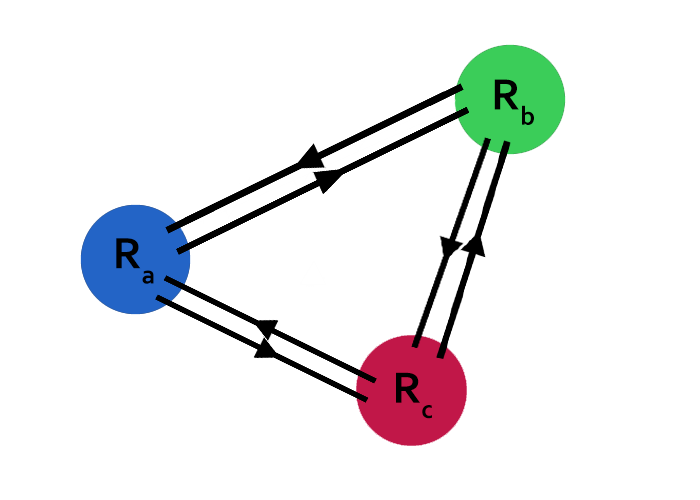
\includegraphics{./figures/abstract_kripke.png}
    \caption[Abstracted Kripke Structure]{Representation of the abstracted Kripke structure of the provided example. This structure is verified with the local model checking algorithm (\autoref{alg:modelchecking}) to ensure satisfaction of the deterministic \mucalc{} specification.} 
\label{fig:abs_kripke}
\end{figure}

To demonstrate the effectiveness of our method, we provide the following pertinent example. We use continuous double integrator dynamics on two spatial dimensions, resulting in a 4D state space. State and control vectors take the form
\begin{equation}
    \vec{x} =  \begin{bmatrix}
                    x \\
                    y \\
                    \dot x \\
                    \dot y
                \end{bmatrix},
    \ \vec{u} =  \begin{bmatrix}
                    u_x \\
                    u_y
                \end{bmatrix}
\end{equation}
and the dynamical system is given by
\begin{equation}
    \dot{\vec{x}} = %\begin{pmatrix}
                        \begin{bmatrix}
                            0 & 0 & 1 & 0 \\
                            0 & 0 & 0 & 1 \\
                            0 & 0 & 0 & 0 \\
                            0 & 0 & 0 & 0 \\
                        \end{bmatrix} \vec{x} +
                        \begin{bmatrix}
                            0 & 0 \\
                            0 & 0 \\
                            1 & 0 \\
                            0 & 1  
                        \end{bmatrix} \vec{u},
                    %\end{pmatrix}
\end{equation}
with initial condition $\vec{x}_0 = [100, 400, 0, 0]$.
We choose the cost function for \gls{sst}* to be the duration of the trajectory, T, along with a control cost term, with cost matrix $R_{sst}$:
\begin{equation}
    J_{SST} = \int_0^\top \left( 1 + u^\top R_{sst} u \right ) dt.
\end{equation}
% Define atomic propositions $a,b,$ and $c$ to be true for state $s$ if and only if $s \in R_a$, or $s \in R_b$, or $s \in R_c$, respectively,
The specification we wish to satisfy is to visit three distinct regions of the state space,
$R_a, R_b$, and $R_c$ infinitely often while avoiding the obstacle regions collectively called $R_o$. Define atomic propositions $p_i$, $i \in \{a, b, c, o\}$, such that ${p_i} \in \mathcal{L}(s)$ if and only if $s \in R_i$. We write the deterministic \mucalc{} formula $\Phi$ as follows
\begin{align*}
    \mu M.[  (\lnot o \land \Diamond M) \lor \\
        \nu W.\{
            ( a &\land \mu X.[\lnot o \land ( ((b \lor c) \land W) \lor \Diamond X)] ) \lor \\
            ( b &\land \mu Y.[\lnot o \land ( ((a \lor c) \land W) \lor \Diamond Y)] ) \lor \\
            ( c &\land \mu Z.[\lnot o \land ( ((a \lor b) \land W) \lor \Diamond Z)] ) \} ].
\end{align*}

Upon running \gls{sst}* in three parallel instances starting in the center of each proposition's associated region in state space, we obtained \autoref{fig:all_trees}. Note that there are six candidate trajectories, each representing the best path from one region to another in terms of the cost, $J_{SST}$. In general, for $p$ positively-appearing atomic propositions in the {\mucalc{}} specification, $p$ trees are incrementally updated in parallel, and we search for ${p-1}$ candidate trajectories for each tree.

The model checking algorithm ensures that at least one cycle of length three may be formed in the abstracted Kripke structure, which itself is constructed with three nodes (one for each proposition region), and whose directed edges represent the candidate trajectories that begin in one proposition region and end in another one. The procedure was run until all six candidate trajectories successfully reached their appropriate goal regions, allowing for the abstracted Kripke structure to be fully connected\footnote{This was done in order to compare the cost associated with each direction of the possible 3-cycle, although \autoref{alg:kinospecplan} as it is written would return as soon as any satisfactory path is found.}. The resulting structure contains two infinite paths satisfying proposition $\Phi$ above, noting that the initial condition is situated in the blue region: (i)\ head to the green region first, then the burgundy region, and returning to the blue region to repeat, or (ii)\ head to the burgundy region first, then the green region, and repeating upon returning to the blue region.

In order to determine which of the cycles to take, a simulation is run using the LQR controller discussed in \autoref{section:lqr}, tracking each of the proposed paths and bridging the gap between the end of one trajectory and the beginning of another. The state-cost matrix $Q$ was set to $\texttt{diag}(25, 25, 25, 25)$ and the control-cost matrix $U$ was chosen to be $\texttt{diag}(1, 1)$. Using total cost to determine the better of the two proposed solutions, it is found that option (i)\ results in a faster circuit between the three regions. See \autoref{fig:sol}.


\begin{figure}
    \centering
    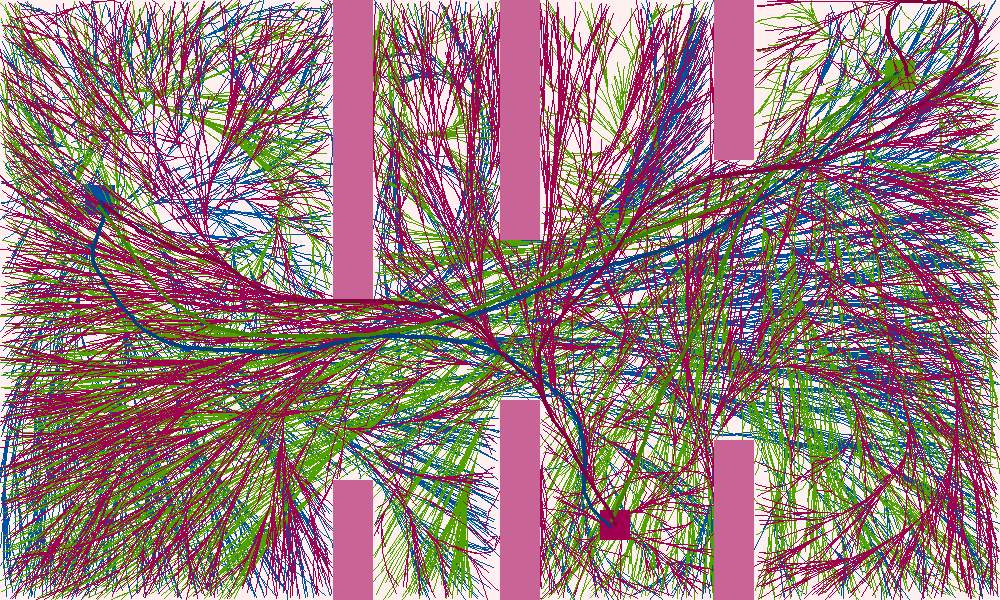
\includegraphics[scale=0.61]{./figures/doubleint2.png}
    \caption[Double Integrator Example --- Three Trees using SST*]{\gls{sst}* is performed three times, producing a Kripke structure for each of the regions shown here in blue (left), burgundy (bottom center), and green (top right). Obstacles are represented as pink rectangles. The color of each line matches the color of the region of the Kripke structure to which it belongs, and the bolded curves are the lowest-cost trajectories that reach another region.} 
    \label{fig:all_trees}
\end{figure}

\begin{figure}
    \centering
    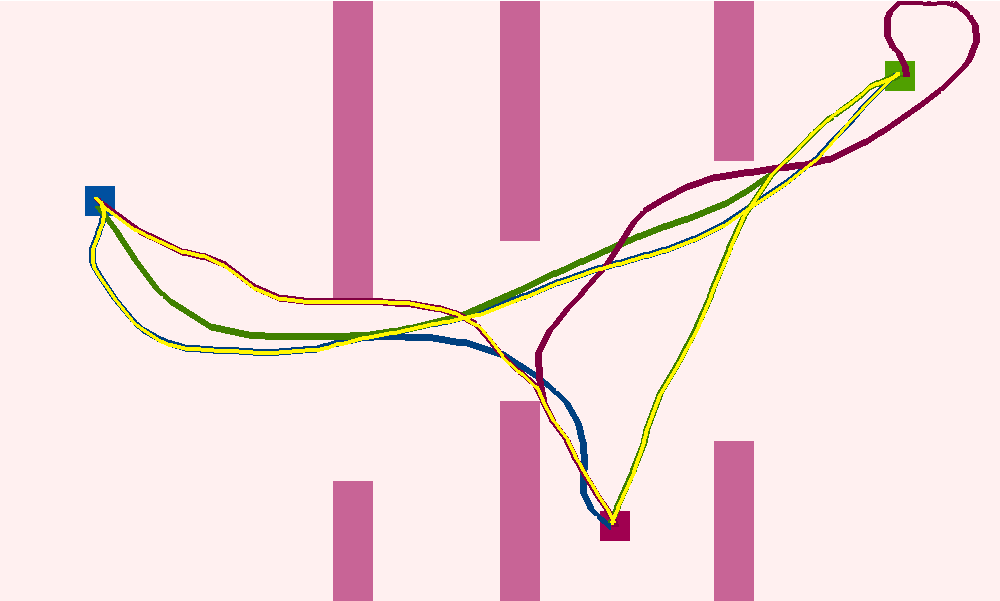
\includegraphics[scale=0.61]{./figures/doubleint2-good-lqr.png}
    \caption[Double Integrator Example --- Simulation Results]{The six candidate trajectories are shown, where curves of the same color are selected from the same Kripke structure. The solution trajectory is shown in yellow, starting in the center of the blue region and tracking the infinite path with least cost that satisfies specification $\Phi$.} 
\label{fig:sol}
\end{figure}


%    \begin{figure}[thpb]
%       \centering
%       \framebox{\parbox{3in}{We suggest that you use a text box to insert a graphic (which is ideally a 300 dpi TIFF or EPS file, with all fonts embedded) because, in an document, this method is somewhat more stable than directly inserting a picture.
% }}
%       %\includegraphics[scale=1.0]{figurefile}
%       \caption{Inductance of oscillation winding on amorphous
%        magnetic core versus DC bias magnetic field}
%       \label{figurelabel}
%    \end{figure}
   

%!TEX root = uw-ethesis.tex
% chktex-file 46 (ignore warnings about $...$)
% chktex-file 24 (ignore \label warning)
% chktex-file 35 (ignore max/min)
% chktex-file 44 (ignore warnings about vertical lines in arrays)
\chapter{Quadrotor Motion Planning}\label{chap:quad}



%%%%%%%%%%%%%%%%%%%%%%%%%%%%%%%%%%%%%%%%%%%%%%%%%%%%%%%%%%%%%%%%%%%%%%%%%%%%%%%%
%%%%%%%%%%%%%%%%%%%%%%%%%%%%%%%%%%%%%%%%%%%%%%%%%%%%%%%%%%%%%%%%%%%%%%%%%%%%%%%%
\section{Quadrotor Model}
%%%%%%%%%%%%%%%%%%%%%%%%%%%%%%%%%%%%%%%%%%%%%%%%%%%%%%%%%%%%%%%%%%%%%%%%%%%%%%%%
%%%%%%%%%%%%%%%%%%%%%%%%%%%%%%%%%%%%%%%%%%%%%%%%%%%%%%%%%%%%%%%%%%%%%%%%%%%%%%%%

Quadrotors, as discussed in \autoref{chap:intro}, are growing in popularity for their many uses. Autonomous navigation for quadrotors is still in the early stages of development, although there are already some basic autonomous behaviours in use commercially; for example, many drones now support following a moving person to capture video footage. What makes quadrotor motion planning a truly interesting challenge is the fact that they occupy a 12D state space, and they are non-holonomic vehicles that are governed by nonlinear dynamics. The combination of high-dimensionality and nonlinearity render many current methods ineffective in the context of motion planning, for example the interval method~\cite{jaulin2001,Li2018}, which discretizes the state and control space with intervals, and suffers from the curse of dimensionality~\cite{Indyk1998}.

Before proceeding to the mathematics involved, it may be of interest to the reader to discuss our choice to use the term ``quadrotor''. But first, we begin by seeing that the word ``helicopter'' can be broken down into ``helico'', which is itself a combining form of ``helix'' (screw), and ``pter'' meaning ``wing''. Some people have referred to four-rotor helicopter UAVs as ``quadcopters'', but this terminology is ignorant of the Ancient Greek etymology of such words, as ``heli/copter'' is not the correct partitioning of the English word. So, the term ``quadrotor'' avoids the issue altogether, and its meaning is self-evident.

Now, in order to overcome the hurdles inherent in motion planning for such a complex system as a quadrotor, Ross Allen and Marco Pavone put forth a ``full-stack approach'' for real-time kinodynamic planning of such aerial vehicles~\cite{Allen2016}. First and foremost, a sampling-based planning approach was deemed necessary to deal with unknown environments online, and while \gls{sst}* can handle the high-dimensionality and nonlinearity of the quadrotor system without needing a steering function, the incremental nature cripples its ability to plan effectively in an online setting. On the other hand, \gls{fmt}, with its pre-sampled states and its flexibility in allowing to perform much of the necessary pre-computation offline, is much more suited to online planning. For this reason, the authors centre their planning framework around a variant of FMT* called \texttt{kinoFMT}, introduced in \autoref{chap:prelims}. Once an approximate trajectory is found using this planning algorithm, trajectory smoothing is applied, and due the differentially flat nature of the quadrotor dynamics, it is then feasible to track the smooth trajectory with the proposed controller.

This chapter begins by analyzing the dynamical system that models quadrotor dynamics. Then, much of the work from~\cite{Allen2016} is described in various levels of detail, and conclusions are drawn from the efficacy of this approach. Finally, the main idea of using high-level temporal logic specifications using an abstracted Kripke structure, presented in \autoref{chap:sstpaper}, is applied to quadrotor kinodynamic planning \emph{with} steering under the aforementioned real-time planning framework.





\subsection{Background}

Before delving into the laws of motion for quadrotor systems, we begin by defining the underlying coordinate systems used in our analysis. In order to describe the position and velocity of the quadrotor, we need a fixed inertial reference frame (sometimes called the world frame) where Newton's laws hold. We will use the usual $x,y,z$ coordinates with basis vectors $\{e_1, e_2, e_3 \}$, where ${e_1 = {[1, 0, 0]}^\top}$, ${e_2 = {[0, 1, 0]}^\top}$, and ${e_3 = {[0, 0, 1]}^\top}$. It is worth noting that much of the aviation/aeronautics literature uses the \gls{ned} configuration, so equations of motion found in that frame will differ slightly from those that we will present here. Along with the inertial frame, we define a body-fixed frame with basis $\{b_1, b_2, b_3\}$ whose origin coincides with the centre of mass of the quadrotor. The vectors $b_1$ and $b_2$ lie in the plane formed by the four rotors, and $b_3$ points in the direction opposite the applied thrust. See \autoref{fig:frames}.

\begin{figure}[ht]
    \centering
    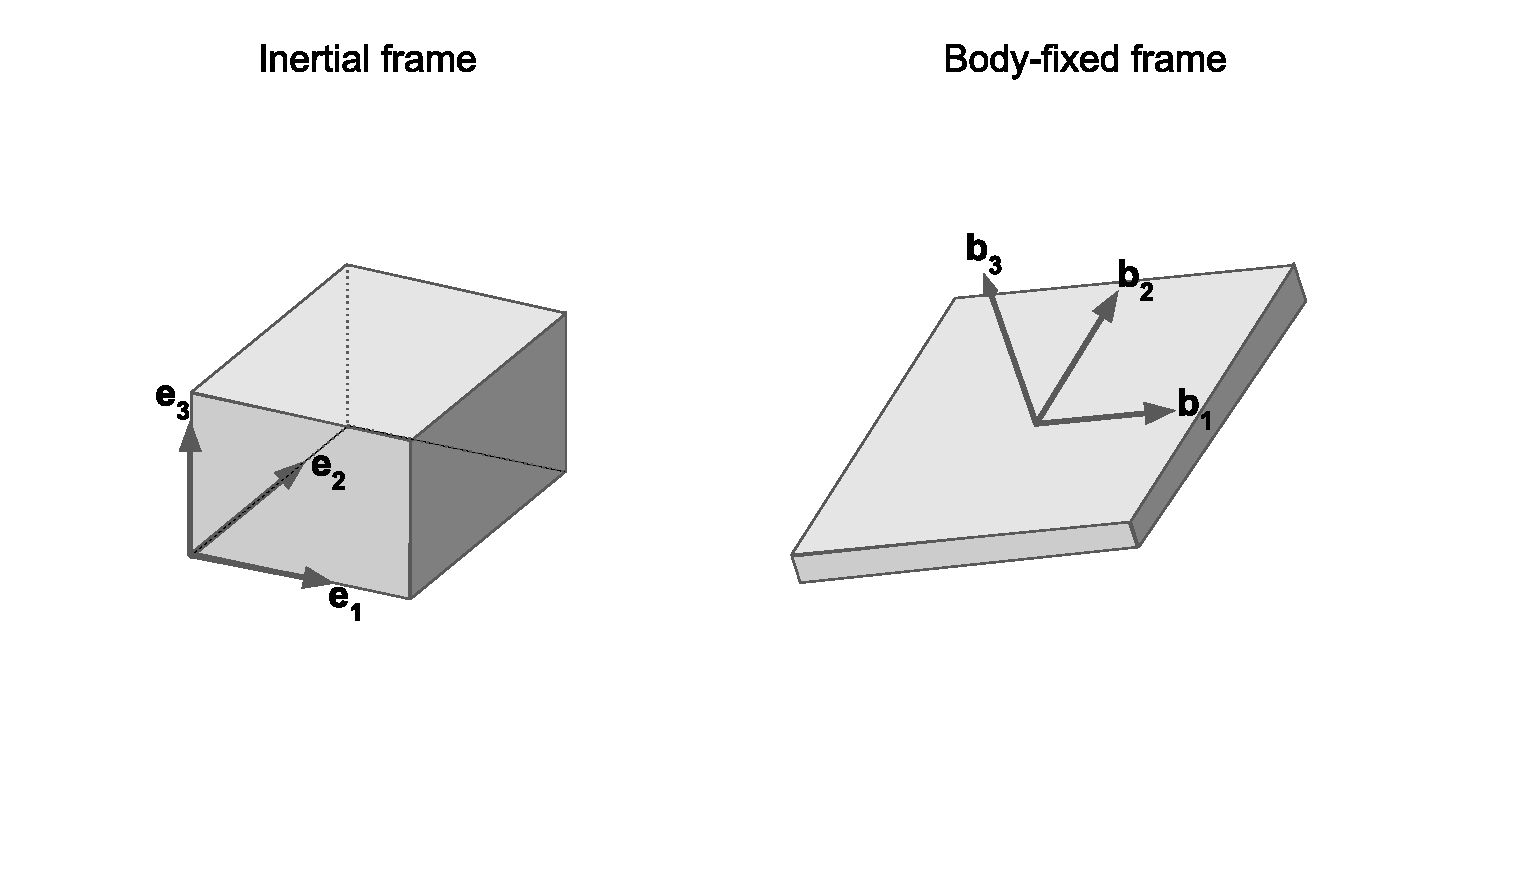
\includegraphics[scale=0.6]{./figures/frames2.eps}
    \caption[Inertial and body-fixed frames]{The inertial frame and the body-fixed frame are shown, where the origin of the body-fixed frame is placed at the centre of mass of the quadrotor, which is represented as a flattened rectangular prism.}
\label{fig:frames}
\end{figure}

Controlling a quadrotor involves adjusting the thrust applied to each of the four rotors. Note that opposite rotors rotate in the same direction, and adjacent rotors rotate in opposite directions; consequently, if all four rotors apply the same amount of thrust, the quadrotor will fly directly upward, and the angular momentum contributed by each rotor cancels so that there is zero rotational motion. Quadrotor motion is described in the space of all rigid body transformations, namely the special Euclidean group $\text{SE}(3)$. This space has six degrees of freedom: translation in three dimensions, and rotation about each of the three body-fixed axes. It bears mentioning that, since there are only four control inputs compared with six degrees of freedom, the quadrotor system is underactuated.

Rotational motion is often described by the Euler angles measuring yaw (about $b_3$), pitch (about $b_2$), and roll (about $b_1$). The use of Euler angles as state variables is not ideal, though, as singularities and jump-discontinuities arise as a result of restricting the domain of such angles. Recent work by Taeyoung Lee et al.\ instead takes a geometric control approach with a globally defined model to avoid many of the issues inherent to Euler angles~\cite{Lee2010}, and we will make use of their work in modeling quadrotor dynamics. The important change they make is to replace the three Euler angle state variables with a single $3 \times 3$ matrix in the special orthogonal group, $\text{SO}(3)$, defined as follows:
\begin{equation}
    \text{SO}(3) = \{ R \in \R^{3 \times 3} \ \vert \ R^\top R = I,\ \det(R) = 1 \}.
\end{equation}
The elements $R \in \text{SO}(3)$ are called rotation matrices, and they are orthogonal matrices that describe the attitude of the quadrotor. Note that the restriction on the determinant of the matrices excludes orthogonal matrices with determinant equal to $-1$, which have the effect of transforming via reflection as opposed to rotation. As we are concerned only with physically possible transformations, reflections are removed from the set of allowed transformation matrices, and the qualifier ``special'' is prepended to the orthogonal group. 

The rotation matrices in $\text{SO}(3)$ are linear transformations that act on vectors via multiplication to produce a rotated vector. Given a vector $\vec{v} \in \R^3$ in the inertial frame (i.e., $v = ae_1 + be_2 + ce_3$ for some $a,b,c \in \R$) and rotation matrix $R \in \text{SO}(3)$, $w=Rv$ is the result of rotating $v$ by $R$, where $w$ is expressed in the inertial frame. A useful interpretation of such rotation matrices is that the matrix $R$ represents the current orientation of a rigid body. That is to say, the body-fixed axes are obtained, as above, by applying the rotation $R$ to each of the basis vectors $e_1, e_2$, and $e_3$. In this way, we need not consider the rotation an active change in the quadrotor's orientation, but rather as the current orientation obtained by rotating the axes of the inertial frame.





\subsection{Dynamics}\label{quad:dynamics}

We are now sufficiently equipped to outline the equations of motion of a quadrotor \gls{uav}. The first equation states the relationship between the position of the centre of mass, ${x={[x_1, x_2, x_3]}^\top \in \R^3}$, and the velocity of the centre of mass, $v={[v_1, v_2, v_3]}^\top \in \R^3$, together constituting the first six state variables. The equation is simply
\begin{equation}
    \dot x = v.\label{quad:dyn:eqn1}
\end{equation}

To develop the next, more interesting, equation, we begin by noticing that $b_3 = Re_3$. If we express the magnitude of the thrust generated by the $i^{th}$ propeller as $f_i,\ i \in \{1,2,3,4\}$, then the total thrust in the body-fixed frame is given by $fb_3$, where $f = \sum_{i=1}^4 f_i$. Therefore, in the inertial frame, the total thrust is written as $fRe_3$. The only other force acting on the quadrotor (ignoring disturbances) is the force of gravity, which pulls along the $-e_3$ axis, and we write the force as $-mge_3$, where $m$ is the mass of the quadrotor, and $g$ is the magnitude of the force of gravity ($g \approx 9.8$ on the surface of the Earth). Using Newton's Second Law, we may now put these forces together to write our second equation of motion,
\begin{equation}
    m\dot v = fRe_3 - mge_3.\label{quad:dyn:eqn2}
\end{equation}

The final two equations of motion for the quadrotor system describe the rotational dynamics. Define $\Omega \in \R^3$ to be the angular velocity of the quadrotor in the body-fixed frame. $R$ and $\Omega$ constitute the remaining state variables, and they appear together in an interesting way in the third equation of motion, which describes the rate at which the rotation matrix changes with time.

Before proceeding, let us first introduce $\mathfrak{so}(3)$, the Lie algebra associated with the Lie group $\text{SO}(3)$. A Lie algebra contains the elements of the tangent space of the Lie group at the identity, and in this case, we have that $\mathfrak{so}(3)$ is simply the set of skew-symmetric matrices,
\begin{equation}
    \mathfrak{so}(3) = \{ X \in \R^{3 \times 3} \ \vert \ X^\top + X = 0 \}.
\end{equation} 
The skew-symmetric matrices represent infinitesimal rotations. Consider rotating a vector $x$ about some unit vector, $v$, by angle $\theta$ in the counterclockwise direction. In the limit as $\theta$ approaches $0$, the rotation occurs normal to the plane containing both vectors, in the direction $v \times x$. This motivates the definition of the \emph{hat map}, $\hat \cdot : \R^3 \to \mathfrak{so}(3)$ which satisfies $\hat a b = a \times b$\ for all $a, b \in \R^3$.
\begin{equation}
    \hat a
    =
    \widehat{
    \begin{bmatrix}
        a_1 \\
        a_2 \\
        a_3
    \end{bmatrix}
    }
    =
    \begin{bmatrix}
        0        &  -a_3 & a_2 \\
        a_3 &  0         & -a_1 \\
        -a_2 & a_1  & 0
    \end{bmatrix}
\end{equation}
Tying these concepts together, the infinitesimal generator of rotation in the given scenario is the matrix $\hat v$, since $\hat v x$ yields the direction of the rotation of $x$ about $v$ by an infinitesimal angle.

Recall that an element $\hat v \in \mathfrak{so}(3)$ is in the tangent space of $\text{SO}(3)$ \emph{at the identity}. In order to produce an infinitesimal rotation at an arbitrary element $R \in \text{SO}(3)$, we simply left-multiply the appropriate infinitesimal rotation (element of $\so(3)$) by $R$. In this case, $\hat \Omega$ is the appropriate element of $\mathfrak{so}(3)$ since $\Omega$ describes the rotational motion, and thus the axis of rotation, of the quadrotor. Therefore, we conclude that the third equation of motion is:
\begin{equation}
    \dot R = R \hat \Omega.\label{quad:dyn:eqn3}
\end{equation}

Finally, the last equation of motion governs how $\Omega$ changes over time. Given the moment of inertia matrix, $J \in \R^{3 \times 3}$, of our quadrotor, we can write an equation for the total torque in the body-fixed frame, $\tau \in \R^{3 \times 3}$ (the rotational analog to the second equation of motion, \autoref{quad:dyn:eqn2}). Following the same line of reasoning in deriving \autoref{quad:dyn:eqn3}, we can see that the rate of change of any one body-fixed frame basis vector, $u \in \{b_1, b_2, b_3\}$, due to the angular velocity is given by
\begin{equation}
    \frac{du}{dt} = \Omega \times u = \hat \Omega u.\label{quad:eqn:dudt}
\end{equation}
For any differentiable vector-valued function $f(t) = f_x(t)b_1 + f_y(t)b_2 + f_z(t)b_3$, we can use \autoref{quad:eqn:dudt} to find the time-derivative of $f$ as follows~\cite{Lanczos1986}:
\begin{align*}
    \frac{df}{dt} &= \frac{df_x}{dt}b_1 + f_x\frac{db_1}{dt}
                    +\frac{df_y}{dt}b_2 + f_y\frac{db_2}{dt}
                    +\frac{df_z}{dt}b_3 + f_z\frac{db_3}{dt} \\
                  &= \frac{df_x}{dt}b_1 + \frac{df_y}{dt}b_2 + \frac{df_z}{dt}b_3
                    +\Omega \times (f_x(t) b_1 + f_y(t) b_2 + f_z(t) b_3) \\
                  &= {\left( \frac{df}{dt} \right)}_b + \Omega \times f(t),
\end{align*}
where ${\left( \frac{df}{dt} \right)}_b$ indicates the derivative of $f$ as seen in the body-fixed frame. Note that an observer in the body-fixed frame does not perceive
The last remaining concept that needs to be defined to obtain the remaining equation of motion is the angular momentum, $L$, which satisfies $L = J\Omega$. The time-derivative of angular momentum is equal to the total torque, $\tau = {[\tau_1, \tau_2, \tau_3]}^\top$ (in the body-fixed frame), which is exactly what we use to determine an equation for $\dot \Omega$.
\begin{align*}
\tau &= \frac{dL}{dt} \\
     &= \frac{d}{dt} J\Omega \\
     &= {\left( \frac{d}{dt} J\Omega \right)}_b + \Omega \times J\Omega \\
     &= J\dot\Omega + \Omega \times J\Omega
\end{align*}
Note that in the last step, since the derivative is taken in the body-fixed frame, the moment of inertia, $J$, does not change, so the term $\dot J\Omega$ resulting from the product rule vanishes. Rearranging, we obtain our final equation of motion:
\begin{equation}
 J\dot \Omega = \tau - \Omega \times J\Omega. \label{quad:dyn:eqn4}
\end{equation}

We summarize the nonlinear dynamics of the deterministic model for quadrotor motion below~\cite{Mellinger2012}.
\begin{equation}
    \begin{aligned}
        \dot x &= v \\
        \dot v &= \frac{f}{m}Re_3 - ge_3 \\
        \dot R &= R \hat \Omega \\
        \dot \Omega &= J^{-1} (\tau - \Omega \times J\Omega)
    \end{aligned}
\label{quad:full_dyn}
\end{equation}

The inputs to this system are $u={[f, \tau_1, \tau_2, \tau_3]}^\top \in \R^m$ with dimension $m=4$, and the state vector is given by $X = {[x, v, R, \Omega]}^\top \in \R^3 \times \R^3 \times \text{SO}(3) \times \R^3$.

Note that the low-level quadrotor controller must convert the input values to the individual torques to be applied to each propeller. We assume that the first and third propellers rotate clockwise, the second and fourth propellers rotate counterclockwise, and that the torque is directly proportional to the thrust generated by a propeller, with proportionality constant $c_\tau$. Recall that $f_i, \ i \in \{1,2,3,4\}$ denote the thrusts generated, and define $d$ to be the distance in the $b_1b_2$-plane from the centre of mass to the centre of each propeller. Then, we can write the inputs as follows~\cite{Lee2010, Mellinger2012}:
\begin{equation}
    \begin{bmatrix}
        f \\ \tau_1 \\ \tau_2 \\ \tau_3
    \end{bmatrix}
    =
    \begin{bmatrix}
        1       & 1       & 1       & 1   \\
        0       & -d      & 0       & d   \\
        d       & 0       & -d      & 0   \\
        -c_\tau & c_\tau  & -c_\tau & c_\tau
    \end{bmatrix}
    \begin{bmatrix}
        f_1 \\ f_2 \\ f_3 \\ f_4
    \end{bmatrix}.
\label{quad:eqn:invert_this}
\end{equation}
Since this matrix is invertible provided $d, c_\tau \neq 0$, it suffices to invert the matrix and multiply by the vector of inputs, $u$, in order to obtain the necessary thrusts, and therefore torques, for the individual propellers.

The remainder of this chapter solves the following problem, as similarly stated in~\cite{Allen2016}, with the addition of satisfying a temporal logic specification.
\begin{problem}
    \  \\
    Let $\mathcal{X}_{free} \subseteq \R^3 \times \R^3 \times \text{SO}(3) \times \R^3$ be the subset of state space that is unobstructed, and let $\mathcal{U} \subseteq \R^4$ be the set of admissible control inputs. Furthermore, let $\Phi$ be a deterministic \mucalc{} specification. Then, given the continuous-time quadrotor dynamical system,
    \begin{equation}
        \dot X(t) = f(X(t), u(t)),\hspace{4mm} X(0) = X_0,\label{quad:generic_sys}
    \end{equation}
    where $f$ is given by the equations of motion in \autoref{quad:full_dyn},
    determine a control signal,
    \begin{equation}
        u(t) = {[f(t), \tau_1(t), \tau_2(t), \tau_3(t)]}^\top \in \mathcal{U},
    \end{equation}
    and corresponding state trajectory, 
    \begin{equation}
        X(t) = {[x(t), v(t), R(t), \Omega(t)]}^\top \in \mathcal{X}_{free}
    \end{equation}
    that satisfies specification $\Phi$, or return failure if such a trajectory is not found.
\label{quad:problem}
\end{problem}




%%%%%%%%%%%%%%%%%%%%%%%%%%%%%%%%%%%%%%%%%%%%%%%%%%%%%%%%%%%%%%%%%%%%%%%%%%%%%%%%
%%%%%%%%%%%%%%%%%%%%%%%%%%%%%%%%%%%%%%%%%%%%%%%%%%%%%%%%%%%%%%%%%%%%%%%%%%%%%%%%
\section{Real-Time Motion Planning}\label{chap:quad:rtmp}
%%%%%%%%%%%%%%%%%%%%%%%%%%%%%%%%%%%%%%%%%%%%%%%%%%%%%%%%%%%%%%%%%%%%%%%%%%%%%%%%
%%%%%%%%%%%%%%%%%%%%%%%%%%%%%%%%%%%%%%%%%%%%%%%%%%%%%%%%%%%%%%%%%%%%%%%%%%%%%%%%

As discussed in \autoref{chap:prelims} and \autoref{chap:sstpaper}, many motion planning algorithms require knowledge of a steering function. \texttt{kinoFMT} (\autoref{alg:fmt}) is one such algorithm, but as previously noted, the nonlinear quadrotor dynamics make it difficult (or perhaps impossible) to find an analytic solution to the \gls{obvp}. In order to apply the \texttt{kinoFMT} algorithm to the problem of kinodynamic planning for a quadrotor, we must therefore use an approximation to the 12D nonlinear system that has a known steering function. The crucial property involved in using an approximation to the full dynamics is called \emph{differential flatness}, which allows any sufficiently smooth path to be tracked. The method employed by Allen et al.~\cite{Allen2016} involves two further important steps: reachable set approximation, and trajectory smoothing. To elaborate, the reachable set approximation is arguably the key step that allows for online planning, as it is used to rapidly connect the initial state and goal states to the preexisting tree that is to be computed beforehand offline. Once a path is planned between the newly added initial state and goal states, a smooth path is generated called a \emph{minimum-snap trajectory}, and we leverage the differential flatness property of the quadrotor dynamics to be able to track this smooth path in the full dynamics. The details involved in tracking are provided, and simulations are performed to demonstrate the effectiveness of this method.





\subsection{Framework Overview}

We now outline the high-level real-time planning framework proposed in~\cite{Allen2016}. The entire process is broken down into two parts: the offline precomputation phase, where as much information as possible is gathered before knowing any of the specific details that will become clear during real-time trials, and the online planning phase, which takes into account the actual initial position and goal region and performs the various planning steps described in later sections.



\subsubsection{Offline Phase}

Before online planning can begin, it is desirable to perform as much precomputation as possible to minimize the computational effort, and therefore the time, required when online. With this in mind, there are three steps to perform offline:
\begin{enumerate}
    \item sampling the state-space,
    \item constructing a cost roadmap,
    \item training a classifier that determines nearest nodes.
\end{enumerate}

The sampling step simply stores a user-defined number of samples, $N$, in a set, $V$. The samples are drawn uniformly from the unobstructed state-space, without any regard for potential obstacles (as such information is as yet unknown). This manner of sampling is a boon to the flexibility of the proposed method, as it can be applied online in a very general setting.

Next, for every pair of states in $V$, the \gls{obvp} is solved. The optimal time and cost are then stored as values in a look-up table (or dictionary), called \texttt{Cost}, associated with the corresponding pair of states. In this way, no computation for cost is required while running \texttt{kinoFMT} online, except when it comes to pairs involving the states known only when online: the initial state and sampled goal states. This issue is addressed in the final step of the offline phase.

Note that as $N$ gets large, the number of pairs grows quadratically as $N(N-1)$, and the bisection optimization method used to compute the optimal time for each pair converges linearly. For $N>2000$, this can be rather expensive, so one could choose to instead sample some number of pairs on which to perform the precomputation. Furthermore, the ordering of the pairs matters, so one cannot use a symmetry argument to halve the number of computations. To illustrate this point, consider two states in one dimension (with 2D state-space: position and velocity), each with some positive velocity. The state that is behind has a fairly straightforward means of reaching the other state, whereas the state that is ahead would be forced to change direction, get to the appropriate position and accelerate in the positive direction once again to reach the desired positive velocity.

In order to avoid having to compute the cost between each of the initial or goal states and the existing $N$ samples, which would involve solving the \gls{obvp} $O(N)$ times, a machine learning approach is implemented. A \gls{svm} is used, learning from the data in the \texttt{Cost} look-up table to rapidly classify a pair of points as ``near'' or ``not near'' in terms of the cost incurred by traveling from one state to the other. As such, the \gls{obvp} must be solved only for those points that are estimated to fall within a certain cost threshold.



\subsubsection{Online Planning}

Upon beginning a trial with a quadrotor, the first step is to sample $N_{goal}$ states from the now-known goal region. Then, given the initial state of the quadrotor, we determine the outgoing nearest neighbours from the initial state using the trained \gls{svm} and store them in $\mathcal{N}_{init}^{out}$, and we similarly determine the incoming neighbours for each of the goal states, storing them in $\mathcal{N}_{goal}^{in}$. At this point, the \gls{obvp} is solved between the initial state (goal states) and the states in its neighbourhood, $\mathcal{N}_{init}^{out}$ ($\mathcal{N}_{goal}^{in}$), and the appropriate entries are added to the cost roadmap, \texttt{Cost}. Note that using the \gls{svm} to estimate cost-limited reachable sets provides an immense reduction in the number of online \gls{obvp} solutions required, from $O(N)$ down to $O(1)$.

Now that the \texttt{Cost} look-up table is complete, the \texttt{kinoFMT} algorithm (\autoref{alg:fmt}) is run on the set of samples, $V$ along with the initial and goal states. The algorithm quickly returns the optimal path from start to goal, excluding any paths that are found to collide with obstacles. However, given that the path is found using an approximated linear model, it must be smoothed so that it may be tracked by leveraging the differential flatness of the quadrotor system. With this aim, a smoothing algorithm takes the waypoints (states) from the path outputted by \texttt{kinoFMT} and produces a set of four high-degree polynomials in the flat output variables that are smooth up to fourth order. Finally, all that remains is to track the smooth path using an appropriately tuned feedback controller.
 



\subsection{Differential Flatness}\label{quad:diff_flat}

We say of a system that it is differentially flat if the states and the inputs can be written as functions of the system's flat outputs and their derivatives. We state the definition more precisely as follows~\cite{Greeff2018}:
\begin{defn}
    Consider a continuous-time nonlinear system $\dot x(t) = f(x(t),u(t)),\ x(0) = x_0$ where $t \in \R$, $x(t) \in \R^n$ is the state, $u(t) \in \R^m$ is the input, and $f$ is a smooth function. This nonlinear system is \emph{differentially flat} if there exists $\zeta(t) \in \R^m$, whose components are differentially independent, such that the following hold~\cite{Fliess1995}:
    \begin{align*}
        \zeta &= \Lambda(x, u, \dot u, \mathellipsis, u^{(\delta)}) \\
            x &= \Phi(\zeta, \dot \zeta, \mathellipsis, \zeta^{(\rho-1)}) \\
            u &= \Psi^{-1}(\zeta, \dot \zeta, \mathellipsis, \zeta^{(\rho)})
    \end{align*}
    where $\Lambda, \Phi, \Psi^{-1}$ are smooth functions, $\zeta = {[\zeta_1, \mathellipsis, \zeta_m]}^\top$ is the vector of \emph{flat outputs}, and $\delta$ and $\rho$ are the maximum orders of the derivatives of $\zeta$ and $u$ necessary in defining the flat outputs and their relation to $x$ and $u$.
\end{defn}
The concept of differential flatness is useful for many reasons, although two in particular seem eminently popular in the field of motion planning. The first is that differential flatness can be used in the process of feedforward (or feedback) linearization to separate a nonlinear system into a linear flat model and a nonlinear transformation, so that is possible to consider the control problem only on the linear part, and the resulting flat states and flat inputs can be used to correct for the nonlinear part via inversion of the nonlinear transformation~\cite{Greeff2018,VanNieuwstadt1998}. The second consequence of differential flatness, and the one we focus on here, is that any smooth trajectory in the flat output space, subject to reasonably bounded derivatives, can be tracked~\cite{Mellinger2011}. The significance of this fact is not to be understated, as even the underactuated quadrotor can track a sufficiently smooth path generated from the flat outputs of the system.

In the case of quadrotors, the flat outputs can be chosen to be the position of the centre of mass in the inertial frame and the yaw angle, $\zeta = {[x_1, x_2, x_3, \psi]}^\top$. Mellinger and Kumar prove that this choice of flat outputs does indeed admit a way to write the state and input as a function of $\zeta$ and its derivatives up to fourth order.



\subsection{Quadrotor Dynamics Approximation}

There exist many known approaches to handling nonlinear dynamics when solving motion planning problems, such as using a planner that avoids the steering problem altogether (e.g., \gls{sst}). Another approach, when dealing with a differentially flat nonlinear system, is to use feedforward linearization, as mentioned in \autoref{quad:diff_flat}. In the method presented here, as in~\cite{Allen2016}, the quadrotor system is first approximated to be the linear double integrator system (\autoref{quad:approxdyn}). The approximation assumes the quadrotor can accelerate in any direction at any time, which, while crude, is sufficient to generate high-quality trajectories from an initial state to a goal region. The idea is that, upon using \texttt{kinoFMT} to generate an ordered set of waypoints on this simplified system, a smooth trajectory in the flat outputs can be generated and tracked in the full dynamics.
\begin{equation}
    \dot{\tilde{x}}(t) = 
    \underbrace{
    \begin{bmatrix}
        0_{3 \times 3} & I_{3 \times 3} \\
        0_{3 \times 3} & 0_{3 \times 3}
    \end{bmatrix}
    }_A \tilde{x}(t)
    +
    \underbrace{
    \begin{bmatrix}
            0_{3 \times 3} \\
            I_{3 \times 3}
    \end{bmatrix}
    }_B  \tilde{u}(t)
    -
    \underbrace{
    \begin{bmatrix}
        0_{5 \times 1} \\
        g
    \end{bmatrix}
    }_c
\label{quad:approxdyn}
\end{equation}
Here, $\tilde{x} = {[x_1, x_2, x_3, \dot{x}_1, \dot{x}_2, \dot{x}_3]}^\top \in \R^6$ is simply a truncated representation of the full state including only position and velocity, and $\tilde{u} = {[\ddot{x}_1, \ddot{x}_2, \ddot{x}_3]}^\top \in \R^3$  is the new control. We denote the matrix multiplying $\tilde{x}(t)$ by $A$, the matrix multiplying $\tilde{u}(t)$ by $B$, and the constant vector by $c$.

Now that we are working with a linear system, we solve the \gls{obvp} as in~\cite{Schmerling2015}. Given any two (sampled) states, we seek an analytic solution to the problem of finding an optimal path between them, as well as the optimal control signal used to generate such a path. We begin by defining the cost function
\begin{equation}
    \mathcal{J}(\tilde{u}, t_{f}) = \int_0^{t_f} 1 + {\tilde{u}(t)}^\top R_u \tilde{u}(t) dt
\label{quad:eqn:cost}
\end{equation}
where $R_u \in \R^{3 \times 3}$ is symmetric positive definite, and $t_f$ is the fixed final time. This cost function prioritizes minimum-time solutions while also penalizing control effort. A suitable choice for the control penalty weighting matrix is $R_u = w_R I_{3 \times 3}$, for some $w_R \in \R$.

Without derivation, the optimal cost for the double integrator \gls{obvp} from initial state $\tilde{x}_0$ at time $t=0$ to $\tilde{x}_1$ at time $t=t_f$ is given by~\cite{Schmerling2015, Allen2016}
\begin{equation}
    \mathcal{J}^*(t_f) =
    t_f + {(\tilde{x}_1 - \underbar{x}(t_f))}^\top {G(t_f)}^{-1} (\tilde{x}_1 - \underbar{x}(t_f)).
\label{quad:eqn:opt_cost}
\end{equation}
The state and control trajectories which achieve this optimal cost are given by
\begin{align}
    \tilde{x}(t) &= \underbar{x}(t) + G(t)\exp(A^\top[t_f - t]){G(t_f)}^{-1} (\tilde{x}_1 - \underbar{x}(t_f)) \\
    \tilde{u}(t) &= R_u^{-1} B^\top \exp(A^\top[t_f - t]){G(t_f)}^{-1} (\tilde{x}_1 - \underbar{x}(t_f))
\end{align}
where
\begin{align}
    \underbar{x}(t) &= \exp(At)x_0 + \int_0^t \exp(As)c\ ds \\
               &= \exp(At)x_0
                  -
                  \begin{bmatrix}
                      0 \\
                      0 \\
                      gt^2/2 \\
                      0 \\
                      0 \\
                      gt
                  \end{bmatrix} \\
    G(t)  &= \int_0^t \exp(As)B R_u^{-1} B^\top \exp(A^\top s)\ ds  \\
          &= \frac{1}{w_R}
          \begin{bmatrix}
            t^3/3   &  0  &  0  & t^2/2 &  0  &  0 \\
            0  &  t^3/3   &  0  &  0  & t^2/2 &  0 \\
            0  &  0  & t^3/3   &  0  &  0  & t^2/2 \\
            t^2/2 &  0  &  0  & t  &  0  &  0 \\
            0  & t^2/2 &  0  &  0  & t  &  0 \\
            0  &  0 & t^2/2 &  0  &  0  & t \\
          \end{bmatrix}.
\end{align}

The only remaining unknown is the final time $t_f = \argmin_{t > 0} \mathcal{J}^*(t)$, which can be found via the bisection method performed on the derivative of the convex function $\mathcal{J}^*$. This involves choosing an initial interval $[a,b]$ in which to check for an optimal solution (e.g., $[0.0001, 100]$) as well as some error tolerance, $\epsilon$. The bisection method is a recursive algorithm that checks to see whether the derivative of the function at $a$ has the same sign as the derivative of the function at the midpoint of the interval, $q$. If it is not the same, recurse on the interval $[a,q]$ since a turning point (i.e., a minimum) exists therein. Similarly, if the derivative at $q$ has a different sign from the derivative at $b$, recurse on $[q,b]$. The algorithm terminates and returns the midpoint once the length of the interval, $b-a$, is less than $\epsilon$, or when the derivative at the midpoint is zero.




\subsection{Reachable Set Approximation}\label{quad:reachable_set}


The problem of finding a state $\tilde{x}_b$ that is nearest to state $\tilde{x}_a$ in a kinodynamic framework is not as simple as finding the state $\tilde{x}_b$ which minimizes the Euclidean distance between $\tilde{x}_a$ and $\tilde{x}_b$. Due to the issue of drift, including the consideration of momentum and angular momentum, distance is insufficient in determining the actual difficulty involved in transiting from one state to another. Instead, the cost is given by \autoref{quad:eqn:cost}, used as the optimality condition for the \gls{obvp}. In the same vein, while geometric planners may use some maximal, distance-based search radius, our kinodynamic planner instead uses a cost-limited reachable set when looking for nearby states. We define such a reachable set from a state $\tilde{x}_a$ with maximum cost $J_{th}$, in the subset of unobstructed state space of the approximate dynamics, $\mathcal{\tilde{X}}_{free}$, and given the set of admissible input signals, $\mathcal{\tilde{U}}$, as follows~\cite{Allen2014}:
\begin{equation}
    R(\tilde{x}_a, \mathcal{\tilde{U}}, J_{th}) = 
        \{ \tilde{x}_b \in \mathcal{\tilde{X}}_{free} \ \vert \ \exists \tilde{u} \in \mathcal{\tilde{U}}, t \in [0, t_f]\ \text{s.t.}\ \tilde{x}(t) = \tilde{x}_b\ \text{and}\ \mathcal{J}(\tilde{u},t) \leq J_{th} \}.
\end{equation}
In words, the cost-limited reachable set contains all unobstructed states that can be reached before the final time, $t_f$, using admissible controls and without exceeding the cost threshold.

The issue posed by real-time planning is that solving the \gls{obvp} from the previously unknown initial state to each of the $N$ sampled states is computationally expensive. This would then have to be repeated for each of the newly sampled goal states, rendering the task of online kinodynamic planning practically infeasible. Even worse, if the number of samples is large and the look-up table \texttt{Cost} does not include the cost between every pair of the $N$ samples, then querying for nearby states requires even more \gls{obvp} solutions. What has been proposed in~\cite{Allen2016} is to use an \gls{svm} classifier to estimate whether any given state lies within the cost threshold, $J_{th}$, of another state. That is, when calling $\texttt{Near\_Forward}(x,V,J_{th})$ from \autoref{alg:fmt}, the \gls{svm} is used to estimate, for each $v \in V$, whether or not $v \in R(x, \mathcal{\tilde{U}}, J_{th})$. Similarly, $\texttt{Near\_Backward}(x,V,J_{th})$ returns the set of states $v$ such that $x \in R(v, \mathcal{\tilde{U}}, J_{th})$.

An \gls{svm} works by consuming a large array of training data, \texttt{arr\_train}, with $n_{train}$ entries called \emph{feature vectors}, as well as an array of $n_{train}$ labels. The idea is to train the supervised learning algorithm on the correct labels to be able to partition the space of feature vectors in such a way as to be able to accurately classify new feature vectors. This partitioning can be accomplished in many ways, such as using a simple linear hyperplane as a boundary, or creating more complex nonlinear boundaries. The boundary that is used is determined by the chosen \emph{kernel} function.

Our implementation uses the scikit-learn package ``svm'' for Python. We begin by determining what should be included in the feature vector. One simple choice for the feature vector that is sufficient for our purposes is to concatenate the pair of states. Given a pair of states $(\tilde{x}_a, \tilde{x}_b)$, $\tilde{x}_a, \tilde{x}_b \in \mathcal{\tilde{X}}_{free} \subseteq \R^6$ (in the approximate dynamics), let the $i^{th}$ feature vector of \texttt{arr\_train} be $p_i = {[\tilde{x}_a^\top, \tilde{x}_b^\top]}^\top$. The corresponding label $y_i$ is equal to 1 if the actual optimal cost from $\tilde{x}_a$ to $\tilde{x}_b$ is less than $J_{th}$, and 0 otherwise. In our work, we found the most success using a polynomial kernel of degree 3. All that remains is to choose an error penalty parameter, $C$, as input to the SVC function from the scikit-learn svm package. As with many machine learning techniques, this step is subject to trial and error. Once chosen, the SVC function can be used to train a classifier. Given a new pair of vectors, one can then construct the appropriate feature vector and run it through the trained classifier to check whether or not the pair satisfies the cost-limited reachability condition.

We encourage interested readers to refer to~\cite{Smola2004} for further details regarding \gls{svm}s. 




\subsection{Trajectory Smoothing}

The path generated by \texttt{kinoFMT} cannot be used directly as it is based on the double integrator dynamics approximation\footnote{Note that if we were to apply a different method that could plan on the full nonlinear dynamics, such as with \gls{sst} (\autoref{chap:sstpaper}), smoothing would not be a necessary step, although it can be useful in improving trajectory quality.}. To use the generated path, we must first create a smooth trajectory in each of the four flat outputs: the three components of position and the yaw angle. We opt to use polynomial interpolation on the waypoints of the path generated by our planning algorithm. This section is primarily based on the work of Richter et al.~\cite{Richter2016}, though many details that are missing from these papers are provided.

To accomplish the task of smoothing, we will use $M$ polynomials of order $N_p$ for each of the four flat output variables. To introduce the topic, we will begin by analyzing how the interpolation task is accomplished for one polynomial segment between two waypoints for a single flat output variable. We will then extend the result to create $M$ polynomials, and the procedure may be repeated for each of the other flat output variables.

Based on the proof that the quadrotor system is differentially flat~\cite{Mellinger2011}, it is shown that four derivatives of the flat outputs are required to express the state and the input. For this reason, we require that each polynomial we construct is continuous up to the fourth derivative. Furthermore, each polynomial must have equal derivatives at shared intermediate waypoints to ensure smoothness of the full trajectory. Despite these restrictions, there remain infinitely many possible polynomials that join successive waypoints. We choose the ``best'' option which we define to be the unique polynomial that minimizes the integral of the square of the snap (fourth derivative) of the polynomial, as shown in \autoref{quad:eqn:Jsnap}.
\begin{equation}
    J_{snap}(T) = \int_0^T P^{(4)}(t)dt = p^\top Q(T) p
\label{quad:eqn:Jsnap}
\end{equation}
Here, $T$ is the fixed final time for the given polynomial segment, which was found when solving the \gls{obvp} and subsequently recording the optimal duration and cost in the \texttt{Cost} roadmap, and $Q$ is the Hessian matrix for the integral expression with respect to the vector of polynomial coefficients, $p$. $P(t)$ is given by
\begin{equation}
    P(t) = \sum_{i=0}^{N_p} p_i t^i \hspace{2mm},
    \hspace{2mm} p = {[p_0, p_1, \mathellipsis, p_{N_p}]}^\top.
\end{equation}
Considering a generic polynomial of order $N_p$, we can take four derivatives and compute the integral of the square of the result to determine an expression for $Q$ from \autoref{quad:eqn:Jsnap}, as in~\cite{Allen2016}:
\begin{equation}
    Q_{ij}(T) = \begin{cases}
                    2\left( \frac{i!j!}{(i-4)!(j-4)!}\frac{T^{i+j-7}}{i+j-7}  \right) & ,\ i \geq 4 \ \land\ j \geq 4 \\
                    0 & ,\ \text{otherwise.}
                \end{cases}
\label{quad:eqn:Q}
\end{equation}
Note that the indexing used in this section will follow the computer science convention, so the top-left entry of a matrix has index $(i,j) = (0,0)$.

Interpolation requires the trajectory to pass through its terminal endpoints. Let $d$ be a vector of the derivatives at the initial waypoint ($d_0$) concatenated with the derivatives at the following waypoint ($d_T$). Some of the derivative values may not be known, however, particularly at intermediate waypoints. Let $\beta$ represent the number of unknown derivatives, and let $\delta$ be the total number of derivatives kept in each of $d_0, d_T$. We will determine an appropriate value for $\delta$ when working on the extended problem involving all $M$ polynomial segments. Note that the unknown derivatives can be left free so that our procedure assigns them optimal values, but they must still satisfy continuity. We can encode the continuity constraints as follows:
\begin{equation}
      Ap = d, \hspace{2mm} \text{with \ }
      A = \begin{bmatrix}
            A_0 \\ A_T
          \end{bmatrix}, \hspace{2mm}
      d = \begin{bmatrix}
            d_0 \\ d_T
          \end{bmatrix}
\label{quad:eqn:constraint}    
\end{equation}  
where
\begin{equation}
    \begin{array}{l l}
        A_{0_{ij}} = \begin{cases}
                        j! & , i = j \\
                        0  & , \text{otherwise}
                     \end{cases}
        \ & \ 
        d_{0_i} = P^{(i)}(0)
        \\~\\
        A_{T_{ij}} = \begin{cases}
                        \frac{j!}{(j-i)!}T^{j-i} & , j \geq i \\
                        0  & , j < i
                     \end{cases}
        
        \ & \
        d_{T_i} = P^{(i)}(T).
        
    \end{array}
\end{equation}
The expressions for $A_0$ and $A_T$ are simply the result of differentiating $P(t)$ and evaluating at $t=0$ and $t=T$, respectively, to determine the appropriate coefficients by which to multiply each of the polynomial coefficients in $p$.

Now, we are left with the problem of minimizing $J_{snap}$ subject to the constraint given in \autoref{quad:eqn:constraint}. This is called a constrained \gls{qp}, and the one we are working with here tends to be numerically unstable when the problem is extended to multiple segments. However, it is possible to reformulate the problem as an unconstrained \gls{qp} by optimizing over the vector of derivatives instead of the polynomial coefficients. All that is required is to invert \autoref{quad:eqn:constraint} to obtain $p = A^{-1}d$, so that we can rewrite \autoref{quad:eqn:Jsnap} as
\begin{equation}
    J_{snap}(T) = d^\top A^{-\top} Q(T) A^{-1}d
\label{quad:eqn:Jsnap2}
\end{equation}
where we use the notation $A^{-\top}$ to denote the transpose of the inverse of matrix $A$. The unconstrained problem does not suffer from the same numerical instability as the constrained problem, so we proceed by extending the optimization over $M$ polynomials with this reformulated problem.

Define $A_{1..M}$ and $Q_{1..M}$ to be block diagonal matrices containing the $A$ and $Q$ matrices (respectively) corresponding to the appropriate polynomial segment; that is, the first block in $A_{1..M}$ ($Q_{1..M}$) contains the matrix $A$ ($Q$) for the polynomial between the initial waypoint and the second waypoint, then the next block on the diagonal corresponds to the polynomial between the second and third waypoint, and so on.

We could proceed in a similar fashion for vector $d$, concatenating all of the derivative vectors to obtain $d_{1..M}$, but this results in a vector with an unorganized mix of known and free derivative values. Instead, we will reorder the vector such that the all of the fixed (known) derivative values appear first, followed by all of the free derivatives that remain to be optimized,
\begin{equation}
    d_{order} = \begin{bmatrix}
                    d_{fix} \\
                    d_{free}
                \end{bmatrix}
                , \hspace{2mm} d_{order} = Cd_{1..M},
\label{quad:eqn:ordering}
\end{equation}
where $C$ is a pseudo-ordering matrix that also encodes continuity. Reordering of the concatenated vector, $d_{1..M}$, works by letting $C$ be the identity matrix with appropriately swapped rows. Encoding continuity involves carefully choosing some entries in $C$ to have value $-1$, so that pairs of elements of $d_{1..M}$ that ought to be equal are subtracted. The difference is forced to evaluate to 0 by placing half of the free derivatives in the vector of fixed derivatives, $d_{fix}$, with value 0, since the derivatives at the end point of one polynomial must be equal to the derivatives of the starting point of the next polynomial. See \autoref{quad:eqn:reordering}. Without loss of generality, we can assume that the unknown values of $d_T$ for polynomial segment $j$ are ``known'' and set to be 0 in $d_{fix}$, while the corresponding unknown elements in $d_0$ for polynomial $j+1$ remain as unknown values in $d_{free}$.
\begin{equation}
     d_{T_i}^j - d_{0_i}^{j+1} = 0 ,\ \text{ since \ } A_T^j p^j = A_0^{j+1} p^{j+1}
\label{quad:eqn:reordering}
\end{equation}
where the subscript $i$ denotes the $i^{th}$ component of the vector, and the superscript $j$ denotes the polynomial segment to which the matrix or vector corresponds, $j \in \{ 0, \mathellipsis, M-1 \}$.

We now return to the question: \emph{what is $\delta$, the number of derivatives that we keep in each} $d_0^j, d_T^j$? Consider the extended constraint equation,
\begin{equation}
    A_{1..M} p_{1..M} = d_{1..M},
\label{quad:eqn:extended_constraint}
\end{equation}
where $p_{1..M}$ is the vector that results from concatenating all of the polynomials coefficients for each of the $M$ polynomials. \autoref{quad:eqn:extended_constraint} is a system of $2\delta M$ equations, since each $d^j = {[d_0^j, d_T^j]}^\top$ contains $2\delta$ derivatives of the $j^{th}$ polynomial, $P_j(t)$. We assume we know all derivatives at the initial and final waypoint, and that we know $\beta$ derivatives at every intermediate waypoint. There are a total of $M+1$ waypoints, and we know all derivatives for two of them, leaving $(M-1)\cdot 2(\delta - \beta)$ unknown derivatives. As discussed, half of these unknowns are identical to the other half, so in total there are in fact only $(M-1)(\delta-\beta)$ unknown derivatives. Moreover, there are $M(N_p + 1)$ unknown polynomial coefficients. Ensuring the problem is never over-constrained, we equate the number of equations and the total number of unknown values and solve for $\delta$ and round down, giving:
\begin{equation}
    \delta = \floor*{\frac{M(N+1) - \beta(M-1)}{M+1}}.
\label{quad:eqn:delta}
\end{equation}

Continuing, we may rewrite $J_{snap}$ in this extended form,
\begin{equation}
    J_{snap}(T) = {\begin{bmatrix}
                        d_{fix} \\
                        d_{free}
                   \end{bmatrix}}^\top
                   C^{-\top} A_{1..M}^{-\top} Q_{1..M}(T) A_{1..M}^{-1} C^{-1}
                   \begin{bmatrix}
                        d_{fix} \\
                        d_{free}
                   \end{bmatrix},
\end{equation}
and we note that, since $C$ is not strictly a permutation matrix, $C^\top \neq C^{-1}$ in general.

Defining $H = C^{-\top} A_{1..M}^{-\top} Q_{1..M}(T) A_{1..M}^{-1} C^{-1}$, we can write an expression for $J_{snap}$ in block matrix form:
\begin{align}
    J_{snap} &= {\begin{bmatrix}
                        d_{fix} \\
                        d_{free}
                   \end{bmatrix}}^\top
                   \begin{bmatrix}
                        H_{00} & H_{01} \\
                        H_{10} & H_{11}
                   \end{bmatrix}
                   \begin{bmatrix}
                        d_{fix} \\
                        d_{free}
                   \end{bmatrix} \\
                &= d_{fix}^\top H_{00} d_{fix} + d_{fix}^\top H_{01} d_{free} +
                   d_{free}^\top H_{10} d_{fix} + d_{free}^\top H_{11} d_{free} \\
    \frac{dJ_{snap} }{d(d_{free})}
                &= d_{fix}^\top H_{01} + d_{fix}^\top H_{10}^\top + 2d_{free}^\top H_{11}^\top. \label{quad:eqn:Jsnap-deriv}
\end{align}
Since each $Q^j$ is symmetric by its definition (\autoref{quad:eqn:Q}), $Q_{1..M}$ is symmetric, so $H$ is also symmetric. Setting \autoref{quad:eqn:Jsnap-deriv} to 0, we can then simplify to obtain an expression for the optimized values of the free derivatives,
\begin{equation}
    d_{free}^* = -H_{11}^{-1} H_{01}^\top d_{fix}.
\label{quad:eqn:dfree*}
\end{equation}


All that remains is to invert the extended constraint equation to solve for the $M(N_p + 1)$ polynomial coefficients:
\begin{equation}
    p_{1..M} = A_{1..M}^{-1} d_{1..M}^* \ , \text{ where}\hspace{3mm}
    d_{1..M}^* = C^{-1}    \begin{bmatrix}
                              d_{fix} \\
                              d_{free}^*
                         \end{bmatrix}.
\label{quad:eqn:final_poly}
\end{equation}





\subsubsection{Smoothing Example}

Consider smoothing a trajectory over three waypoints ($M=2$ polynomials): the initial state, the final state, and one intermediate state. Suppose we want to interpolate with polynomials of degree $N_p = 3$, and assume that we know $\beta = 1$ derivatives (i.e., only the actual value; we have no knowledge of the first or any subsequent derivatives) at the intermediate state. Using \autoref{quad:eqn:delta}, we determine $\delta = 2$. Then, \autoref{quad:eqn:extended_constraint} becomes,
% \begin{equation}
%     % A_{1..M}
%     \sbox0{$\begin{array}{c c c c}
%                     1 & 0 & 0 & 0 \\
%                     0 & 1 & 0 & 0 \\
%                     \hline
%                     1 & T_0 & T_0^2 & T_0^3 \\
%                     0 & 1 & 2T_0 & 3T_0^2
%                 \end{array}$}
%     \sbox1{$\begin{array}{c c c c}
%                     1 & 0 & 0 & 0 \\
%                     0 & 1 & 0 & 0 \\
%                     \hline
%                     1 & T_1 & T_1^2 & T_1^3 \\
%                     0 & 1 & 2T_1 & 3T_1^2
%                 \end{array}$}
%     \left[ 
%     \begin{array}{c|c}
%         \vphantom{\usebox{0}}\makebox[\wd0]{\huge $A^0$}&\makebox[\wd0]{\huge $0$} \\
%         \hline
%         \vphantom{\usebox{0}}\makebox[\wd0]{\huge $0$}&\makebox[\wd0]{\huge $A^1$}
%     \end{array}
%     \right]
%     %p_{1..M}
%     \left[
%     \begin{array}{c}
%         p_0^0 \\
%         p_1^0 \\
%         p_2^0 \\
%         p_3^0 \\
%         \hline
%         p_0^1 \\
%         p_1^1 \\
%         p_2^1 \\
%         p_3^1
%     \end{array}
%     \right]
%     =
%     %d_{1..M}
%     \left[
%     \begin{array}{c}\def\arraystretch{1.5}
%         d_{0_0}^0 \\
%         d_{0_1}^0 \\
%         \hline
%         d_{T_0}^0 \\
%         d_{T_1}^0 \\
%         \hline
%         d_{0_0}^1 \\
%         d_{0_1}^1 \\
%         \hline
%         d_{T_0}^1 \\
%         d_{T_1}^1 \\
%     \end{array}
%     \right]
% \label{quad:eqn:matrix_eqn}
% \end{equation}
\begin{equation}
    \left[
    \begin{array}{c c}
        A^0 & 0 \\
        0 & A^1
    \end{array}
    \right]
    \left[
    \begin{array}{c}
        p^0 \\
        p^1
    \end{array}
    \right]
    =
    \left[
    \begin{array}{c}
        d^0 \\
        d^1
    \end{array}
    \right]
\label{quad:eqn:matrix_eqn}
\end{equation}

\[
A^0 = 
\begin{tikzpicture}[baseline=0cm,mymatrixenv] 
    \matrix[mymatrix] (m)  {
        1 & 0 & 0 & 0 \\
        0 & 1 & 0 & 0 \\
        1 & T_0 & T_0^2 & T_0^3 \\
        0 & 1 & 2T_0 & 3T_0^2 \\
    };
    \mymatrixbraceright{1}{2}{$A_0^0$}
    \mymatrixbraceright{3}{4}{$A_T^0$}
\end{tikzpicture}
,\hspace{5mm} 
A^1 = 
\begin{tikzpicture}[baseline=0cm,mymatrixenv] 
    \matrix[mymatrix] (m)  {
        1 & 0 & 0 & 0 \\
        0 & 1 & 0 & 0 \\
        1 & T_1 & T_1^2 & T_1^3 \\
        0 & 1 & 2T_1 & 3T_1^2 \\
    };
    \mymatrixbraceright{1}{2}{$A_0^1$}
    \mymatrixbraceright{3}{4}{$A_T^1$}
\end{tikzpicture}
\]

\[
p^0 = 
\begin{tikzpicture}[baseline=0cm,mymatrixenv] 
    \matrix[mymatrix] (m)  {
        p_0^0 \\
        p_1^0 \\
        p_2^0 \\
        p_3^0 \\
    };
\end{tikzpicture}
,\hspace{5mm} 
p^1 = 
\begin{tikzpicture}[baseline=0cm,mymatrixenv] 
    \matrix[mymatrix] (m)  {
        p_0^1 \\
        p_1^1 \\
        p_2^1 \\
        p_3^1 \\
    };
\end{tikzpicture}
,\hspace{5mm} 
d^0 = 
\begin{tikzpicture}[baseline=0cm,mymatrixenv] 
    \matrix[mymatrix] (m)  {
        d_{0_0}^0 \\
        d_{0_1}^0 \\
        d_{T_0}^0 \\
        d_{T_1}^0 \\
    };
    \mymatrixbraceright{1}{2}{$d_0^0$}
    \mymatrixbraceright{3}{4}{$d_T^0$}
\end{tikzpicture}
,\hspace{5mm} 
d^1 = 
\begin{tikzpicture}[baseline=0cm,mymatrixenv] 
    \matrix[mymatrix] (m)  {
        d_{0_0}^1 \\
        d_{0_1}^1 \\
        d_{T_0}^1 \\
        d_{T_1}^1 \\
    };
    \mymatrixbraceright{1}{2}{$d_0^1$}
    \mymatrixbraceright{3}{4}{$d_T^1$}
\end{tikzpicture}
\]
where $T_0, T_1$ are the final times for the first and second segments, respectively, and we start the clock back at $t=0$ for each new segment. The polynomials we seek to find are of the form $P_j(t) = \sum_{i=0}^{N_p} p_i^j t^i $, for $j \in \{ 0,1 \}$. Please note that the subscripts $T_0$, $T_1$ of the derivative values do not refer to the final times, but rather to the indices of vectors $d_T^0$ and $d_T^1$.

Determining the reordering matrix involves first deciding how to order $d_{1..M}$ into a vector of the form ${[d_{fix}, d_{free}]}^\top$. Recalling that $\beta = 1$, and since there is only one intermediate waypoint, only two values are unknown (but equal): $d_{T_1}^0$ and $d_{0_1}^1$. As discussed, we can set $d_{T_1}^0$ to be a ``known'' value, 0, so that 
\begin{equation}
d_{order} = 
\begin{tikzpicture}[baseline=0cm,mymatrixenv] 
    \matrix[mymatrix] (m)  {
        d_{fix} \\
        d_{free} \\
    };
\end{tikzpicture}
=
\begin{tikzpicture}[baseline=0cm,mymatrixenv] 
    \matrix[mymatrix] (m)  {
        d_{0_0}^0 \\
        d_{0_1}^0 \\
        d_{T_0}^0 \\
        d_{T_1}^0 \\
        d_{0_0}^1 \\
        d_{T_0}^1 \\
        d_{T_1}^1 \\
        d_{0_1}^1 \\
    };
    \mymatrixbraceright{1}{7}{$d_{fix}$}
    \mymatrixbraceright{8}{8}{$d_{free}$}
\end{tikzpicture}
\end{equation}
and the corresponding pseudo-ordering matrix is given by,
\begin{equation}
C = {}
    \begin{bmatrix}
        1 & 0 & 0 & 0 & 0 & 0 & 0 & 0 \\
        0 & 1 & 0 & 0 & 0 & 0 & 0 & 0 \\
        0 & 0 & 1 & 0 & 0 & 0 & 0 & 0 \\
        0 & 0 & 0 & 1 & 0 & -1 & 0 & 0 \\
        0 & 0 & 0 & 0 & 1 & 0 & 0 & 0 \\
        0 & 0 & 0 & 0 & 0 & 0 & 1 & 0 \\
        0 & 0 & 0 & 0 & 0 & 0 & 0 & 1 \\
        0 & 0 & 0 & 0 & 0 & 1 & 0 & 0
    \end{bmatrix}
\end{equation}
which satisfies \autoref{quad:eqn:ordering}. The $-1$ entry corresponds to the single unknown, $d_{0_1}^1$, which must be equal to $d_{T_1}^0$. Upon multiplying $Cd_{1..M}$, the two values are subtracted, and the corresponding value in $d_{fix}$ is chosen to be 0 to enforce the continuity constraint. This same method can be applied for any number of unknown but equal pairs at intermediate waypoints.

We could then proceed to apply \autoref{quad:eqn:dfree*} to compute $d_{free}^*$, which ultimately allows us to find the polynomial coefficients, $p_{1..M}$, using \autoref{quad:eqn:final_poly}. Given that this is a toy example, however, the small degree of polynomials used ($N_p = 3$) implies that the snap, i.e., fourth derivative, is always zero, so there is nothing meaningful to minimize. The purpose of this example is to elucidate the method used. On the other hand, larger problems, while more pertinent, lead to unwieldy matrix equations best left for a programming environment.

A reasonable concern is that the new smooth trajectory may now intersect with obstacles. During the original path planning performed by \texttt{kinoFMT}, any transitions that would lead to a collision were discarded, meaning there must exist a path that successfully navigates the obstacles. To handle the issue of possible collisions, we can therefore successively add waypoints at the midpoints of the segment in which a collision is detected, and the smoothing operation is performed every time a new waypoint is added. In this way, the smooth trajectory can lie as close as is necessary to the path found using \texttt{kinoFMT}~\cite{Richter2016}.

As a final remark, recall that the smoothing procedure must produce a set of polynomials for each of the flat outputs: $x_d = {[x_{1_d}, x_{2_d}, x_{3_d}]}^\top$, the desired $x, y, z$ position, and $\psi_d$, the desired yaw angle. While the position of the waypoints is contained directly in the waypoint states of the approximated system, the yaw angle is not. In practice, the yaw angle can be specified by the user. Some common choices include maintaining a constant heading, $\psi_d = \psi_0 \in \R$, or facing in the direction of travel, using $\psi_d = \arctan(\dot{x}_{2_d}/\dot{x}_{1_d})$.





\subsection{Tracking Controller}\label{quad:tracking}

Leveraging the differential flatness of the quadrotor system, we can use a feedback controller to track any smooth path with reasonably bounded derivatives, such as the path generated using the trajectory smoothing technique above. In this section, the geometric tracking controller developed in~\cite{Lee2010} is presented along with some clarifying details.



\subsubsection{Tracking Errors}

The first step involved in designing our tracking controller is to define the tracking errors. Recall that the full state of the quadrotor dynamical system is given by $X = {[x,v,R,\Omega]}^\top$. The errors for the position and velocity are simply:
\begin{align}
    e_x &= x - x_d, \\
    e_v &= v - v_d,
\end{align}
where the vector $x_d = {[x_{1_d}, x_{2_d}, x_{3_d}]}^\top$ is the desired position, as determined by the polynomial trajectories generated in the smoothing step, and $v_d = \dot{x}_d$ is the desired velocity.

Determining an error vector for the orientation, $R$, requires more careful consideration due to the nonlinear nature of the spaces in which $R$ and $R_d$ evolve, where $R_d$ represents the desired rotation matrix, i.e., the desired orientation of the quadrotor. Consider the following error function on $\SO(3)$,
\begin{equation}
    \Psi(R,R_d) = \frac{1}{2}\tr(I - R_d^\top R).
\label{quad:eqn:error_SO3}
\end{equation}

Let us investigate some properties of this function in order to provide some guarantees about the derivation of the tracking controller that follows. Let $S = R_d^\top R \in \SO(3)$. Then by orthogonality, all eigenvalues of $S$ lie on the complex unit circle, and since $S$ is real, any complex eigenvalues come as conjugate pairs. In the case that all eigenvalues are real, since ${\det(S)=1}$ and since, for any matrix, the determinant is the product of the eigenvalues, it must be that $\lambda_i = 1 \text{ or } {-1},\ i \in \{1,2,3\}$, where $\lambda_i$ are the eigenvalues of $S$. Since $\tr(S) = \lambda_1 + \lambda_2 + \lambda_3$, and because there must be an even number of negative eigenvalues to ensure the determinant is positive, we therefore have that $-1 \leq tr(S) \leq 3$. Now consider the case where there is a pair of complex conjugate eigenvalues, $\lambda_2 = \bar{\lambda_1}$. Then $1 = \det(S){=\lambda_1 \lambda_2 \lambda_3} {= \abs{\lambda_1}^2 \lambda_3 } {= \lambda_3}$. Thus, $\tr(S) = 2\mathfrak{R}(\lambda_1) + \lambda_3$ which implies $-1 \leq \tr(S) \leq 3$~\cite{stackexchangeSO3}. In both cases, we obtain the same conclusion, and this result implies that the error function provided in \autoref{quad:eqn:error_SO3} satisfies $0 \leq \Psi(R,R_d) \leq 2$. From this we can glean that $\Psi(R,R_d)$ is always positive if $R \neq R_d$. In the other extreme, when $\tr(R_d^\top R) = -1$ so that $\Psi(R,R_d) = 2$, we can see that $R, R_d$ must differ by a rotation angle of $180^\circ$. The tracking controller developed in~\cite{Lee2010} guarantees that the zero equilibrium of the tracking errors is exponentially attractive provided that, initially, $\Psi(R,R_d) < 2$.

Our goal is to find an expression for $R$ that minimizes the error, $\Psi(R,R_d)$. We begin by defining the \emph{Frobenius inner product} for real matrices $A,B$ of equal dimension:
\begin{equation}
    \frob{A}{B} = \tr(A^\top B).
\end{equation}
This inner product satisfies the product rule from differential calculus, and we use it to rewrite $\Psi(R,R_d)$ as
\begin{equation}
    \Psi(R,R_d) = \frac{1}{2}(3 - \frob{R_d}{R}),
\end{equation}
by linearity of the trace. Then, proceeding with the usual calculus procedure of minimization, with $dR = R\hat{\eta}$ for arbitrary unit vector $\eta \in \R^3$ ($\hat{\eta} \in \so(3)$) as the axis of rotation, as discussed in \autoref{quad:dynamics}, we compute the infinitesimal element of $\Psi$ with respect to $R$:
\begin{align}
    D_R \Psi(R,R_d) 
        &= -\frac{1}{2}(\frob{0, R} + \frob{R_d}{dR}) \\
        &= -\frac{1}{2}\tr(R_d^\top R\hat{\eta}) \label{quad:eqn:DRtrace1} \\
        &= -\frac{1}{2}\tr(\hat{\eta}^\top R^\top R_d), &\tr(A) = \tr(A^\top)  \\
        &= \frac{1}{2}\tr(\hat{\eta} R^\top R_d), &\hat{\eta}^\top = -\hat{\eta} \\
        &= \frac{1}{2}\tr(R^\top R_d \hat{\eta}), &\tr{ABC} = \tr{BCA}. \label{quad:eqn:DRtrace2}
\end{align}
By the equality of \autoref{quad:eqn:DRtrace1} and \autoref{quad:eqn:DRtrace2}, we proceed to obtain
\begin{align}
    D_R \Psi(R,R_d)
        &= -\frac{1}{4}[\tr(\underbrace{R_d^T R - R^\top R_d}_{\hat{e}_R})\hat{\eta}] \\
        &= \frac{1}{2}\frob{\hat{e}_R}{\hat{\eta}}, &-\frac{1}{2}\tr(\hat{x}\hat{y}) = x^\top y
\end{align}
where we defined the quantity 
\begin{equation}
    \hat{e}_R = R_d^T R - R^\top R_d,
\end{equation}
which is necessarily an element of $\so(3)$ since $\hat{e}_R^\top = -\hat{e}_R$. Setting $D_R \Psi(R,R_d) = 0$, and since $\eta$ is an arbitrary axis of rotation, we see that $e_R$ is an appropriate choice of error vector for the attitude of the quadrotor~\cite{Lee2010}. In defining $e_R$, we use the inverse of the hat map, the \emph{vee map}, $\vee{\cdot} : \mathfrak{so}(3) \to \R^3$, which acts on a skew symmetric matrix and returns a vector, $a$, satisfying $\hat{a}b = a \times b$, for all $b \in \R^3$.

Lastly, we seek an error vector for the angular velocity. Begin by noticing that ${\dot{R} \in T_R \SO(3)}$ and ${\dot{R}_d \in T_{R_d} \SO(3)}$ lie in different tangent spaces. Left-multiplying an element of $T_{R_d}\SO(3)$ by the inverse of the element at which we centre the tangent bundle, $R_d^T$, results in an element of the tangent space at the identity, $T_{I}SO(3)$. Left-multiplying this result by $R$, we obtain an element of $T_R\SO(3)$. So, in order to compare $\dot{R}$ and $\dot{R}_d$ in the same tangent space, we proceed as follows:
\begin{align}
    \dot{R} - R R_d^\top \dot{R}_d
        &= R\hat{\Omega} - R R_d^\top R_d \hat{\Omega}_d, 
            &\dot{R} = R \hat{\Omega} \\
        &=  R(\hat{\Omega} - \hat{\Omega}_d), 
            & R_d^\top R_d = I \\
        &= R{(\Omega - \Omega_d)}^\wedge
\end{align}
where the last line follows from the fact that the hat map is distributive. From this, we can see that the expression is 0 if the vector $\Omega - R^\top R_d \Omega_d = 0$, so this becomes the error vector for the angular velocity:
\begin{equation}
    e_\Omega = \Omega - \Omega_d
\end{equation}
Note that, while this seems like the obvious choice, some subtlety is involved in ensuring it is sensible. This same procedure is used by Lee et al.\ in~\cite{Lee2010}, except that the authors converted $R_d$ to the tangent space centered at $R$ using right-multiplication, resulting in a slightly more complex expression for $e_\Omega$.


\subsubsection{Control Laws}

Now that the tracking errors have been defined, we begin to formulate the the tracking controller as in~\cite{Lee2010,Mellinger2012}. We define the desired thrust vector using the second equation of motion of the dynamical system, \autoref{quad:dyn:eqn2}, which we solve for the total thrust term (with the desired acceleration). In designing the full desired thrust vector, we include the position and velocity errors, as the thrust vector is directly responsible for correcting the translational position and velocity. This yields:
\begin{align}
    F &= fRe_3 = m\ddot{x}_d + mge_3, &\text{total (desired) thrust} \\
    F_d &= F - K_x e_x - K_v e_v, &\text{desired thrust with error}
\end{align}
where $k_x, k_v$ are positive definite control gain matrices. Assuming $\norm{F_d} \neq 0$, we can find the desired third body-fixed axis, $b_{3,d}$, as the unit vector in the direction of $F_d$,
\begin{equation}
    b_{3_d} = \frac{F_d}{\norm{F_d}}.
\end{equation}
Since we also have access to the desired yaw angle, $\psi_d$, as it is a flat output for which we constructed a polynomial trajectory, we can write:
\begin{equation}
    b_{1_c} = {[\cos(\psi_d),\ \sin(\psi_d),\ 0]}^\top. 
\end{equation}
This is an intermediate value that we use to define the desired second body-fixed axis, relying on the right-handedness of our coordinate systems:
\begin{equation}
    b_{2_d} = \frac{b_{3_d} \times b_{1_c}}{\norm{b_{3_d} \times b_{1_c}}}.
\end{equation}
The desired first body-fixed axis can then be defined similarly as
\begin{equation}
    b_{1_d} = b_{2_d} \times b_{3_d},
\end{equation}
and the desired rotation matrix can simply be expressed by placing these three basis vectors into a $3 \times 3$ matrix,
\begin{equation}
    R_d = [b_{1_d}, b_{2_d}, b_{3_d}].
\end{equation}

Next, we must find an expression for the desired angular velocity. The result is derived in~\cite{Mellinger2011} and reiterated in the \gls{ned} frame in~\cite{Allen2016}. We include the pertinent results here for completeness.
\begin{equation}
    \Omega_d = \Omega_{1_d} b_{1_d} + \Omega_{2_d} b_{2_d} + \Omega_{3_d} b_{3_d}
\end{equation}
where we define the following useful quantities
\begin{align}
    u_{1_{ff}} &= F \cdot Re_3 \\
    h_\Omega &= \frac{m}{u_{1_{ff}}} [(x_d^{(3)} \cdot b_{3_d})b_{3_d} - x_d^{(3)}].
\end{align}
The feedforward thrust, $u_{1_{ff}}$, projects the total desired thrust onto the current third body-fixed axis. Note that if the actual orientation is $90^\circ$ from the total desired thrust (without the correcting error terms), $u_{1_{ff}}$ is zero as the body must be rotated before the thrust can be used to correct the error. We use $h_\Omega$ to define the components of the desired angular velocity as follows:
\begin{equation}
    \begin{aligned}
        \Omega_{1_d} &= -h_\Omega \cdot b_{2_d} \\
        \Omega_{2_d} &= h_\Omega \cdot b_{1_d} \\
        \Omega_{3_d} &= \dot{\psi}_d (e_3 \cdot b_{3_d}).
    \end{aligned}
\end{equation}

The tracking controller we present here is almost identical to the one developed by Mellinger et al.~\cite{Mellinger2011}. Some small differences exist due to our choice of tracking error vectors and minor sign changes in some definitions above. We choose the control torque, $\tau$, used by Mellinger et al.\ as it omits some complexity from~\cite{Lee2010}, which was found to be unnecessary in practice\footnote{All examples we have tried perform excellently with the simple expression for the control torque, although this does not necessarily imply that the complexity of the controller in~\cite{Lee2010} is never useful. Large errors may benefit from the feedforward terms involving angular acceleration as well as the consideration of a non-diagonal moment of inertia matrix.}. Instead, the control torque vector relies exclusively on the attitude and angular velocity tracking errors and their respective gain matrices, $K_R, K_\Omega$.
\begin{align}
    f &= -(m\ddot{x}_d + mge_3 - K_x e_x - K_v e_v) \cdot Re_3\\
    \tau &= K_R e_R + K_\Omega e_\Omega.
\label{quad:eqn:control_law}
\end{align}
Recall that these four components of the controller, $u={[f, \tau^\top]}^\top$, can be converted into the necessary rotor torques via inversion of \autoref{quad:eqn:invert_this}.

Since the orientation error, $e_R$, is not based on problematic Euler angles, no small angle approximation is used and singularities are avoided. This means that tracking is feasible even for very large deviations in orientation, except when the quadrotor body is completely inverted (exactly $180^\circ$ from the desired orientation). Proof of almost global exponential attractiveness of a similar controller is provided in~\cite{Lee2010}, given that:
\begin{equation}
    \norm{e_\Omega (0)}^2 < \frac{2}{\lambda_{min}(J)}k_R \left( 1 - \frac{1}{2}\tr[I - R_d^\top(0)R(0)] \right)
\end{equation}
where $K_R = k_r I$.





\subsection{Simulations}


Now that the method has been introduced in detail, we are ready to present simulation results.

First, we perform all of the necessary offline computation on four $10 \times 10 \times 10$ environments, where we choose $N_p = 200, 200, 1000, 2000$ samples, and cost threshold $J_{th} = 300, 260, 200, 150$, respectively. We choose decreasing values of $J_{th}$ as the number of samples increases since more samples implies a higher probability of reachable states; as such, we attempt to keep the number of online \gls{obvp} computations to a minimum while still connecting to a sufficient number of points in the tree. Note that we have precomputed the entire \texttt{Cost} look-up table for each configuration, so that the solution to the \gls{obvp} for every pair of sampled points is known before online initiation.

When online, we choose the initial state to be $x_0 = (1.5, 1, 0, 0, 0, 0)$ (starting from rest) and the goal region is defined as the $1 \times 1 \times 2$ rectangular prism whose front-bottom-left corner is positioned at (6,9,8). Moreover, each goal region is explicitly sampled $m = 5$ times to ensure a variety of possible goal states. We also include two large obstacles. The quadrotor is constrained to stay within the bounding box, and must avoid colliding with obstacles.

\begin{figure}
    \centering
    \hspace*{-4.7cm}
    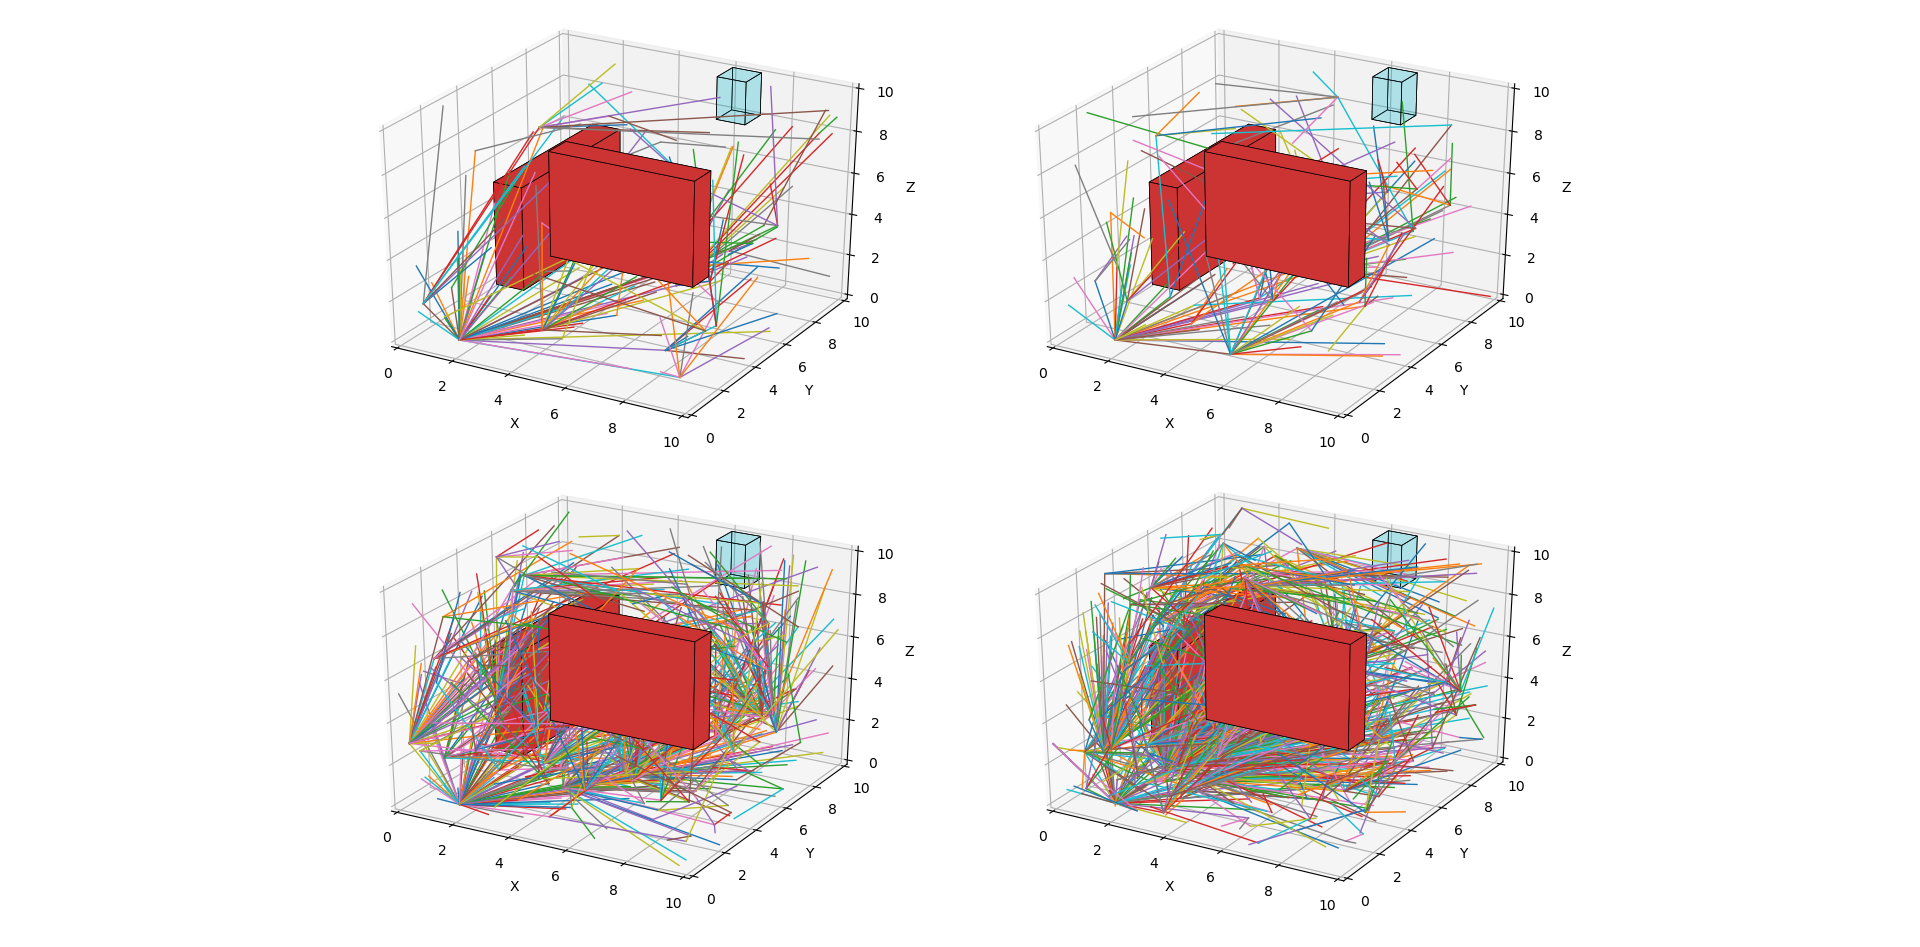
\includegraphics[scale=0.5]{./figures/sim_all_lines}
    \caption[Quadrotor simulation tree]{Shown here are the tree structures generated for four different configurations. Obstacles are in red, and the goal space is in cyan. The top-left and top-right depict the $N_p = 200$ cases with $J_{th} = 300$ and $260$, respectively. The bottom-left is on $N_p = 1000$ samples with $J_{th} = 200$, and the bottom-right uses $N_p = 2000$ samples with $J_{th} = 150$. Edges represent collision-free paths between pairs of possible waypoints. Note that the visualization software always displays an unobstructed view of at least one 3D object, giving the false impression that no edges exist in front of the clearly visible obstacle.}
\label{quad:fig:sim_all_lines}
\end{figure}

Upon running the online planning framework, and before smoothing is applied, we see the result of running \texttt{kinoFMT} in \autoref{quad:fig:sim_waypoints}. Each is the minimum cost path from initial state to goal region for the provided set of random samples. The case with $N_p = 200$ and the lower cost threshold, $J_{th} = 260$ was the fastest, taking 4.8 seconds, 0.95 seconds of which was incurred due to expensive collision checks which are considerably faster in physical experiments (sensors can be queried very rapidly). 

\begin{figure}
    \centering
    \hspace*{-4.7cm}
    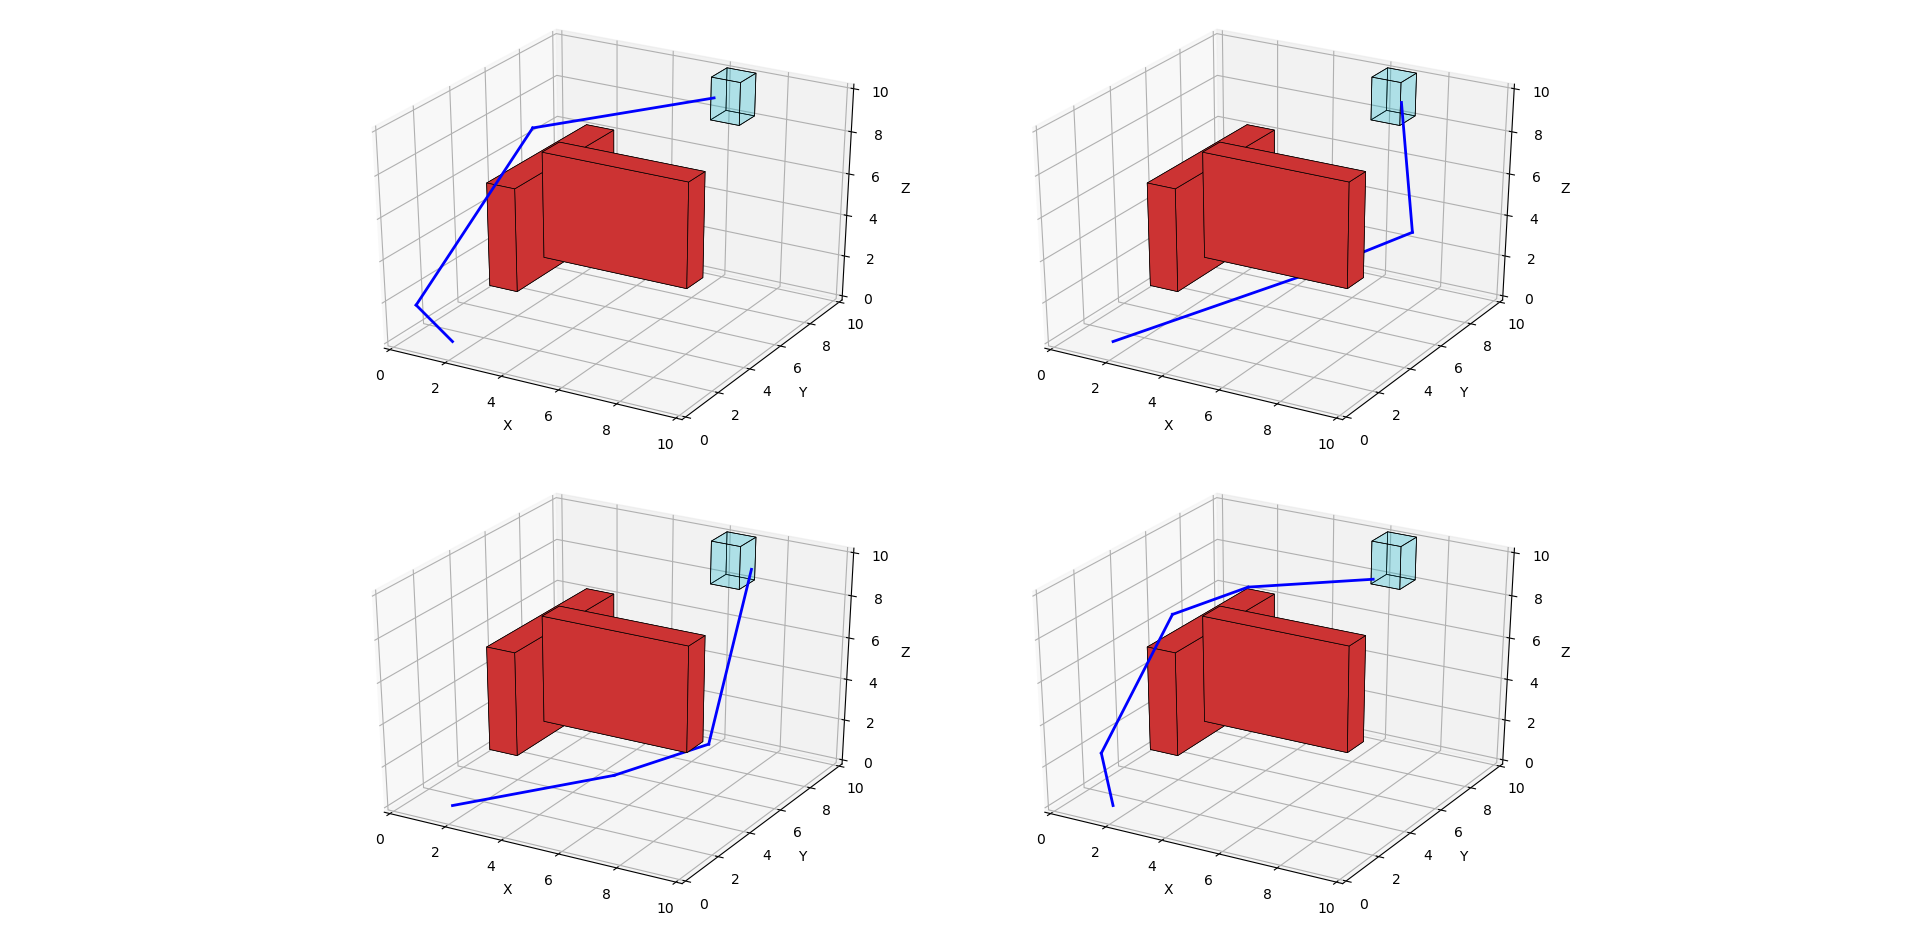
\includegraphics[scale=0.5]{./figures/sim_waypoints}
    \caption[Quadrotor simulation waypoints]{Here we see the best-path waypoints as seen before smoothing is applied. \texttt{kinoFMT} returns a piecewise-linear path connecting the waypoints returned, shown in blue. The four configurations appear in the same order as in \autoref{quad:fig:sim_all_lines}.}
\label{quad:fig:sim_waypoints}
\end{figure}

Trajectory smoothing is run on the same configurations to obtain \autoref{quad:fig:sim_smoothing}.

\begin{figure}
    \centering
    \hspace*{-4.7cm}
    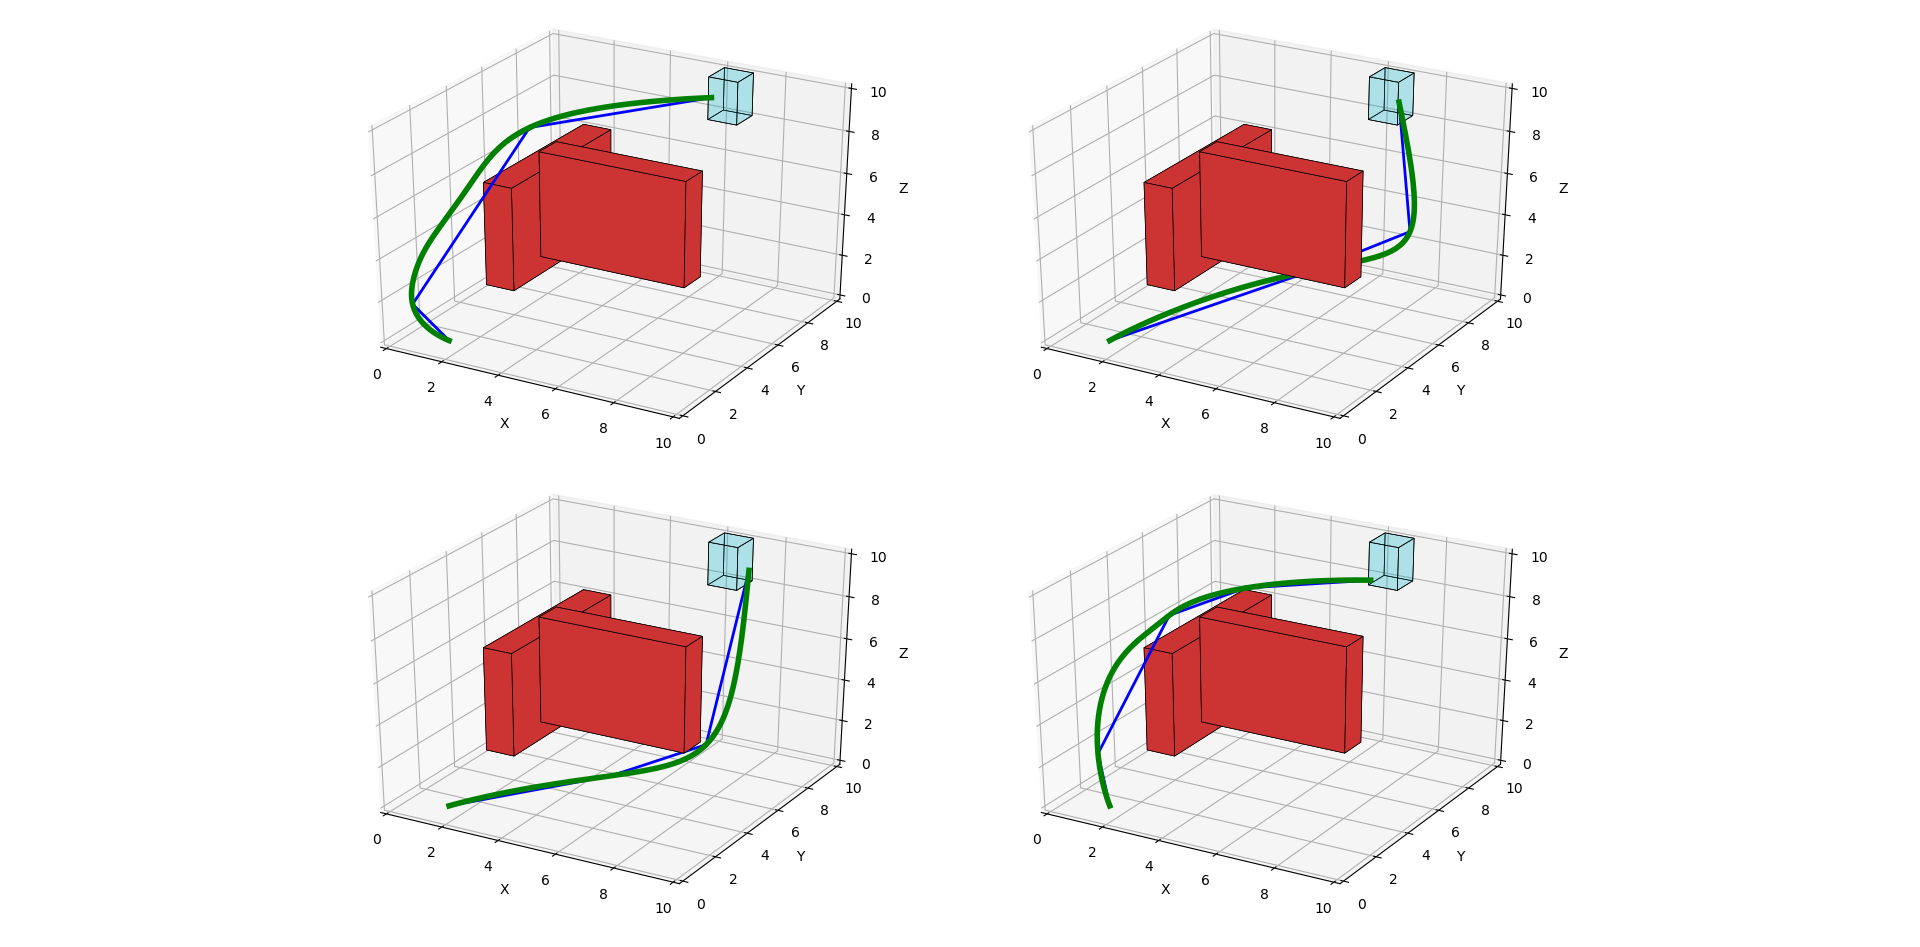
\includegraphics[scale=0.5]{./figures/sim_smoothing}
    \caption[Quadrotor simulation smooth trajectory]{Upon running the trajectory smoothing algorithm, we obtain the green curves shown here. Note that the curve always intersects the piecewise linear path (blue) at the waypoints.}
\label{quad:fig:sim_smoothing}
\end{figure}

Finally, we demonstrate the effectiveness of the tracking controller presented in \autoref{quad:tracking}. The implementation of the tracking controller involves defining a function for the system dynamics from \autoref{quad:full_dyn}. Doing so allows us to forward integrate from the initial state using the control law from \autoref{quad:eqn:control_law}. Numerical integration is performed using the scipy.integrate.ode class with method set to ``vode'' which is the \emph{real-valued variable-coefficient ordinary differential equation} solver. As we demonstrate only a simulation, the control inputs $f$ and $\tau$ can be used directly, so the actual rotor torques need not be computed.

The physical parameters are chosen to closely approximate a very small quadrotor, such as the one used in~\cite{Luis2016}. As such, the mass is set to $m=0.3$ kilograms, and the moment of inertia matrix is diagonal, letting $J=0.00002 I$, with units $Kg\cdot m^2$. Upon tuning the controller with appropriate gain matrices $K_x, K_v, K_R, K_\Omega$, we are able to track the smooth path very closely, as shown in \autoref{quad:fig:sim_tracking}. 

\begin{figure}
    \centering
    \hspace*{-4cm}
    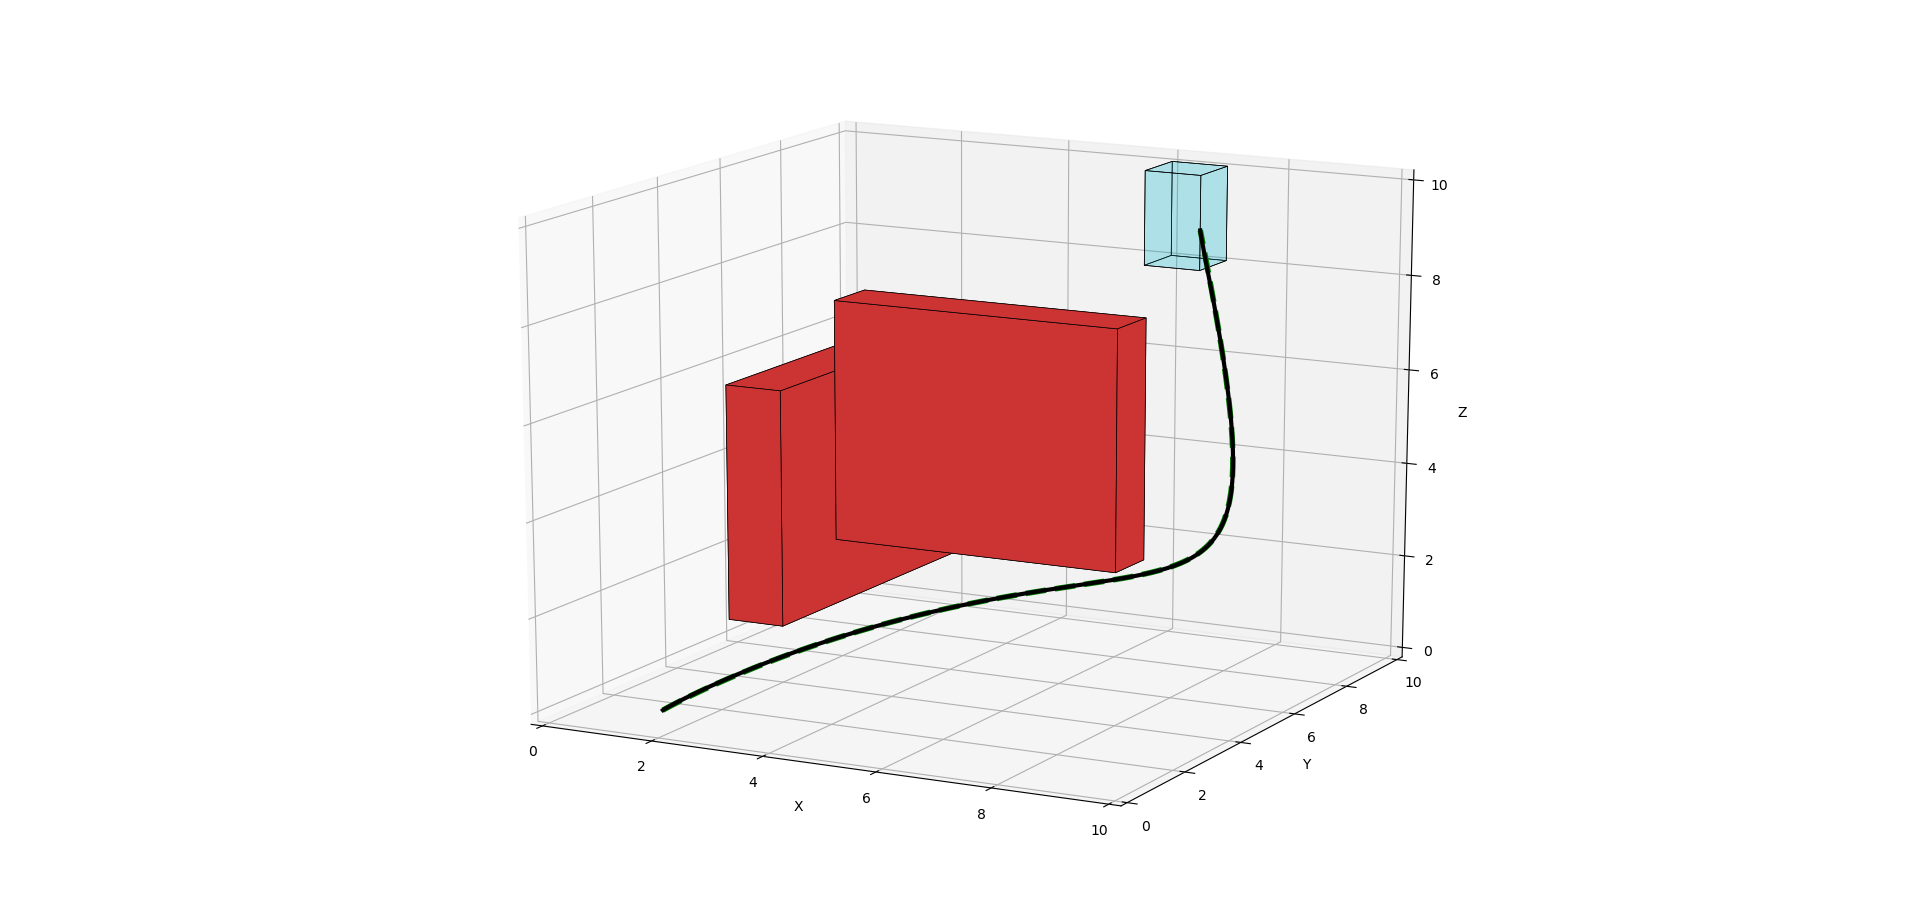
\includegraphics[scale=0.5]{./figures/sim_tracking}
    \caption[Quadrotor simulation trajectory tracking]{Tracking the polynomial trajectory generated for the $N_p = 200$, $J_{th}=260$ configuration (top-right instance of \autoref{quad:fig:sim_smoothing}). The nominal trajectory is shown as a dashed green line, though it is obscured by the simulated trajectory obtained using the tracking controller (black).}
\label{quad:fig:sim_tracking}
\end{figure}

% TODO: include step response?


%%%%%%%%%%%%%%%%%%%%%%%%%%%%%%%%%%%%%%%%%%%%%%%%%%%%%%%%%%%%%%%%%%%%%%%%%%%%%%%%
%%%%%%%%%%%%%%%%%%%%%%%%%%%%%%%%%%%%%%%%%%%%%%%%%%%%%%%%%%%%%%%%%%%%%%%%%%%%%%%%
\section{Abstracted Kripke Structures for Online Planning}
%%%%%%%%%%%%%%%%%%%%%%%%%%%%%%%%%%%%%%%%%%%%%%%%%%%%%%%%%%%%%%%%%%%%%%%%%%%%%%%%
%%%%%%%%%%%%%%%%%%%%%%%%%%%%%%%%%%%%%%%%%%%%%%%%%%%%%%%%%%%%%%%%%%%%%%%%%%%%%%%%

In \autoref{chap:sstpaper}, we introduced the notion of an abstracted Kripke structure which acts as a simplified map, describing how the state-space can be traversed to reach various goal regions. It was shown that the motion planning algorithm \gls{sst}* could be used to incrementally generate trajectories to multiple proposition regions. These solutions could then each be stored as a directed edge in the abstracted Kripke structure, so that the details of the trajectory could be ignored while model checking, thereby greatly improving efficiency. The primary benefit, however, is being able to determine a sequence of trajectories that together can be used to satisfy a temporal logic specification. 

% TODO: why am I not using the method from Chap 3?
This section will use the same concept of an abstracted Kripke structure to construct solution trajectories for a quadrotor system. We will apply the method described in the last section, but instead using the \texttt{kinoFMT} planner with path smoothing, to quickly determine a high-quality trajectory satisfying a given \mucalc{} specification, $\Phi$.

\subsection{Algorithm} 

The meta-algorithm we propose is similar to \texttt{kinoSpecPlan} (\autoref{alg:kinospecplan}). Differences arise due to the fact that \texttt{kinoFMT} is not an incremental algorithm; instead, samples are drawn during the offline phase so that the \texttt{Cost} look-up table can be precomputed. Another key difference is that, unlike \gls{sst}, the use of \texttt{kinoFMT} assumes there is a way to locally steer between points, and the smoothing polynomials can be used to exactly traverse desired waypoints. Since it is only possible to reach sampled states with this method, there are a finite number of possible goal states for any given proposition region. We will use this fact to our advantage, reducing some of the uncertainty arising from tracking in the method presented in \autoref{chap:sstpaper}.

To begin, states are sampled from each of the proposition regions of state space until each such region contains exactly $m$ samples. (Recall that a proposition region consists of the set of states $\brackets{\pi_i}$, where $\pi_i \in \abs{\Pi_+(\Phi)}$, as defined in \autoref{chap:sstpaper:main}). We first plan trajectories from the initial state to each of the proposition regions. Then, for each of the proposition regions, repeat this process, planning from each of the $m$ samples of the region to every other proposition region. In the end, there will be at most $mn(n-1)$ trajectories between proposition regions, and $n$ possible trajectories from the initial state.

Next, we construct the abstracted Kripke structure. A directed edge is added between proposition regions $\brackets{\pi_i}, \brackets{\pi_j}$ only if each of the $m$ samples in $\brackets{\pi_i}$ successfully finds a trajectory to $\brackets{\pi_j}$. % TODO

The idea remains the same whether the proposition regions are known online or offline, although repeating the entire real-time framework can become costly as the number of required \gls{obvp} solutions grows. If the proposition regions are known beforehand, the $m$ samples of each region can be added to the existing tree, and all of the necessary \gls{obvp} solutions can be found offline. In this way, the online planner need only connect the initial state to the existing graph. The bottleneck in this case becomes running \texttt{kinoFMT} up to $n+mn(n-1)$ times. Janson et al.\ showed in~\cite{Janson2015} that \gls{fmt} has time complexity $O(n\log(n))$, and by the same arguments, \texttt{kinoFMT} has the same computational complexity. Altogether, the time complexity contributed by calls of \texttt{kinoFMT} in this new framework is $O(mn^3 \log(n))$. Note that path smoothing is required only for those paths which are required in satisfying the deterministic \mucalc{} specification.



% TODO
%======================================================================

%----------------------------------------------------------------------
% END MATERIAL
%----------------------------------------------------------------------

% B I B L I O G R A P H Y
% -----------------------

% The following statement selects the style to use for references.  It controls the sort order of the entries in the bibliography and also the formatting for the in-text labels.
\bibliographystyle{plain}
% This specifies the location of the file containing the bibliographic information.  
% It assumes you're using BibTeX (if not, why not?).
\cleardoublepage % This is needed if the book class is used, to place the anchor in the correct page,
                 % because the bibliography will start on its own page.
                 % Use \clearpage instead if the document class uses the "oneside" argument
\phantomsection  % With hyperref package, enables hyperlinking from the table of contents to bibliography             
% The following statement causes the title "References" to be used for the bibliography section:
\renewcommand*{\bibname}{References}

% Add the References to the Table of Contents
\addcontentsline{toc}{chapter}{\textbf{References}}

\bibliography{../library}
% Tip 5: You can create multiple .bib files to organize your references. 
% Just list them all in the \bibliogaphy command, separated by commas (no spaces).

% The following statement causes the specified references to be added to the bibliography% even if they were not 
% cited in the text. The asterisk is a wildcard that causes all entries in the bibliographic database to be included (optional).
% \nocite{*}

% The \appendix statement indicates the beginning of the appendices.
\appendix
% Add a title page before the appendices and a line in the Table of Contents
\chapter*{APPENDICES}
\addcontentsline{toc}{chapter}{APPENDICES}
%======================================================================
\chapter[PDF Plots From Matlab]{Matlab Code for Making a PDF Plot}
\label{AppendixA}
% Tip 4: Example of how to get a shorter chapter title for the Table of Contents 
%======================================================================
\section{Using the GUI}
Properties of Matab plots can be adjusted from the plot window via a graphical interface. Under the Desktop menu in the Figure window, select the Property Editor. You may also want to check the Plot Browser and Figure Palette for more tools. To adjust properties of the axes, look under the Edit menu and select Axes Properties.

To set the figure size and to save as PDF or other file formats, click the Export Setup button in the figure Property Editor.

\section{From the Command Line} 
All figure properties can also be manipulated from the command line. Here's an example: 
\begin{verbatim}
x=[0:0.1:pi];
hold on % Plot multiple traces on one figure
plot(x,sin(x))
plot(x,cos(x),'--r')
plot(x,tan(x),'.-g')
title('Some Trig Functions Over 0 to \pi') % Note LaTeX markup!
legend('{\it sin}(x)','{\it cos}(x)','{\it tan}(x)')
hold off
set(gca,'Ylim',[-3 3]) % Adjust Y limits of "current axes"
set(gcf,'Units','inches') % Set figure size units of "current figure"
set(gcf,'Position',[0,0,6,4]) % Set figure width (6 in.) and height (4 in.)
cd n:\thesis\plots % Select where to save
print -dpdf plot.pdf % Save as PDF
\end{verbatim}

\end{document}
